\documentclass[a4paper, traditabstract]{aa} 
%\documentclass[twocolumn]{aa}  

%\pdfoutput=1
\usepackage{fixltx2e}
\usepackage[english]{babel}
\usepackage{graphicx,amsmath}
\usepackage{epstopdf}
\usepackage{epsf,color}
\usepackage[mathscr]{eucal}
\usepackage{amsmath}
\usepackage{amssymb,amsfonts}
\usepackage{natbib}
\usepackage{graphicx}
\usepackage{txfonts}
\usepackage{dsfont}
\usepackage[breaklinks, citecolor=blue, linkcolor=Mygreen, urlcolor=Mypink, colorlinks=true, debug, baseurl=' ']{hyperref}
\usepackage{float}
\usepackage{color}
\usepackage{scrextend}
\usepackage{nccmath}
\usepackage{mathtools, cuted}
\usepackage{lscape}


\definecolor{Mygreen}{rgb}{0.00, 0.72, 0.0}
\definecolor{Mypink}{rgb}{1.0, 0.0, 0.5}
\definecolor{Blue}{rgb}{0.,0.,1.}
\definecolor{LightSkyBlue}{rgb}{0.691,0.827,1.}
\definecolor{Red}{rgb}{1.,0.,0.}
\definecolor{Green}{rgb}{0.,1.,0.}
\definecolor{purple}{rgb}{0.5, 0., 0.5}
\definecolor{nico}{rgb}{0.15,0.,1}
\definecolor{Black}{rgb}{0., 0., 0.}

\newcommand{\nika}{{\it NIKA}}
\newcommand{\nikad}{{\it NIKA2}}
\newcommand{\nico}{\color{nico}}

%\usepackage{lipsum, color}

%\DeclareSIUnit\parsec{pc}
%\DeclareSIUnit\erg{erg}
%\DeclareSIUnit\deg{deg^{-2}}
%\DeclareSIUnit\count{cnt}

\def\intk#1{\displaystyle\int\frac{d^2k_{#1}}{(2\pi)^2}}
\def\intr#1{\displaystyle\int d^2r_{#1}}
\def\simlt{\lower.5ex\hbox{$\; \buildrel < \over \sim \;$}}
\def\simgt{\lower.5ex\hbox{$\; \buildrel > \over \sim \;$}}
\def\NIKA{\textit{NIKA}}
\def\Skydip{\textit{Skydip}}

\bibpunct{(}{)}{;}{a}{}{,}

\bibliographystyle{aa}

\begin{document}

\title{Polarimetry at millimeter wavelengths with the \nika\ camera: calibration  and performance.}
\author{A. Ritacco\inst{1} \and N. Ponthieu \inst{2} \and A. Catalano \inst{1} \and NIKA Core Team}
\institute{
Laboratoire de Physique Subatomique et Cosmologie, Universit\'{e} Grenoble-Alpes, CNRS/IN2P3, 53, rue des Martyrs, 38026 Grenoble Cedex, France
\and
IPAG: Institut de Plan\'{e}tologie et d'Astrophysique de Grenoble, Universit\'{e} Grenoble Alpes, IPAG, F-38000 Grenoble, France, CNRS, IPAG, F-38000 Grenoble, France
}

%\author{R.~Adam \inst{\ref{OCA},\ref{LPSC},\ref{CEFCA}}\thanks{Corresponding author: R\'emi Adam, \url{remi.adam@oca.eu}}
\and O.~Hahn\inst{\ref{OCA}}						%NCT
\and  F.~Ruppin \inst{\ref{LPSC}}
\and  P.~Ade \inst{\ref{Cardiff}}
\and  P.~Andr\'e \inst{\ref{CEA}}
\and M.~Arnaud\inst{\ref{CEA}}					%NCT
\and I.~Bartalucci\inst{\ref{CEA}}					%NCT
\and  A.~Beelen \inst{\ref{IAS}}
\and  A.~Beno\^it \inst{\ref{Neel}}
\and  A.~Bideaud \inst{\ref{Neel}}
\and  N.~Billot \inst{\ref{IRAME}}
\and  O.~Bourrion \inst{\ref{LPSC}}
\and  M.~Calvo \inst{\ref{Neel}}
\and  A.~Catalano \inst{\ref{LPSC}}
\and  G.~Coiffard \inst{\ref{IRAMF}}
\and  B.~Comis \inst{\ref{LPSC}}
\and  A.~D'Addabbo \inst{\ref{Neel},\ref{Roma}}
\and  F.-X.~D\'esert \inst{\ref{IPAG}}
\and  S.~Doyle \inst{\ref{Cardiff}}
\and C.~Ferrari\inst{\ref{OCA}}						%NCT
\and  J.~Goupy \inst{\ref{Neel}}
\and  C.~Kramer \inst{\ref{IRAME}}
\and  G.~Lagache \inst{\ref{LAM}}
\and  S.~Leclercq \inst{\ref{IRAMF}}
\and  J.-F.~Lestrade \inst{\ref{LERMA}}
\and  J.F.~Mac\'ias-P\'erez \inst{\ref{LPSC}}
\and G.~Martinez Aviles\inst{\ref{OCA}}				%NCT
\and D.~Martizzi\inst{\ref{Berkeley}}					%NCT
\and S.~Maurogordato\inst{\ref{OCA}}				%NCT
\and  P.~Mauskopf \inst{\ref{Cardiff},\ref{Arizona}}
\and  F.~Mayet \inst{\ref{LPSC}}
\and  A.~Monfardini \inst{\ref{Neel}}
\and  F.~Pajot \inst{\ref{IAS}}
\and  E.~Pascale \inst{\ref{Cardiff}}
\and  L.~Perotto \inst{\ref{LPSC}}
\and  G.~Pisano \inst{\ref{Cardiff}}
\and E.~Pointecouteau\inst{\ref{IRAP}, \ref{UniToulouse}}%NCT
\and  N.~Ponthieu \inst{\ref{IPAG}}
\and G.W.~Pratt\inst{\ref{CEA}}					%NCT
\and  V.~Rev\'eret \inst{\ref{CEA}}
\and M.~Ricci\inst{\ref{OCA}}						%NCT
\and  A.~Ritacco \inst{\ref{IRAME}}
\and  L.~Rodriguez \inst{\ref{CEA}}
\and  C.~Romero \inst{\ref{IRAMF}}
\and  H.~Roussel \inst{\ref{IAP}}
\and  K.~Schuster \inst{\ref{IRAMF}}
\and  A.~Sievers \inst{\ref{IRAME}}
\and  S.~Triqueneaux \inst{\ref{Neel}}
\and  C.~Tucker \inst{\ref{Cardiff}}
\and H.-Y.~Wu\inst{\ref{CalTech}}					%NCT
\and  R.~Zylka \inst{\ref{IRAMF}}}

\institute{
  Laboratoire Lagrange, Universit\'e C\^ote d'Azur, Observatoire de la C\^ote d'Azur, CNRS, Blvd de l'Observatoire, CS 34229, 06304 Nice cedex 4, France
  \label{OCA}
  \and
  Laboratoire de Physique Subatomique et de Cosmologie, Universit\'e Grenoble Alpes, CNRS/IN2P3, 53, avenue des Martyrs, Grenoble, France
  \label{LPSC}
    \and
  Centro de Estudios de F\'isica del Cosmos de Arag\'on (CEFCA), Plaza San Juan, 1, planta 2, E-44001, Teruel, Spain
  \label{CEFCA}
  \and
Institut de RadioAstronomie Millim\'etrique (IRAM), Grenoble, France
  \label{IRAMF}
\and
Laboratoire AIM, CEA/IRFU, CNRS/INSU, Universit\'e Paris Diderot, CEA-Saclay, 91191 Gif-Sur-Yvette, France 
  \label{CEA}
\and
Astronomy Instrumentation Group, University of Cardiff, UK
  \label{Cardiff}
\and
Institut d'Astrophysique Spatiale (IAS), CNRS and Universit\'e Paris Sud, Orsay, France
  \label{IAS}
\and
Institut N\'eel, CNRS and Universit\'e Grenoble Alpes, France
  \label{Neel}
\and
Institut de RadioAstronomie Millim\'etrique (IRAM), Granada, Spain
  \label{IRAME}
\and
Dipartimento di Fisica, Sapienza Universit\`a di Roma, Piazzale Aldo Moro 5, I-00185 Roma, Italy
  \label{Roma}
\and
Univ. Grenoble Alpes, CNRS, IPAG, F-38000 Grenoble, France 
  \label{IPAG}
    \and
Aix Marseille Universit\'e, CNRS, LAM (Laboratoire d'Astrophysique de Marseille) UMR 7326, 13388, Marseille, France
  \label{LAM}
\and
School of Earth and Space Exploration and Department of Physics, Arizona State University, Tempe, AZ 85287
  \label{Arizona}
\and
Universit\'e de Toulouse, UPS-OMP, Institut de Recherche en Astrophysique et Plan\'etologie (IRAP), Toulouse, France
  \label{IRAP}
\and
CNRS, IRAP, 9 Av. colonel Roche, BP 44346, F-31028 Toulouse cedex 4, France 
  \label{IRAP2}
\and
University College London, Department of Physics and Astronomy, Gower Street, London WC1E 6BT, UK
  \label{UCL}
\and 
Institut d'Astrophysique de Paris, Sorbonne Universit\'es, UPMC Univ. Paris 06, CNRS UMR 7095, 75014 Paris, France 
  \label{IAP}
\and 
LERMA, CNRS, Observatoire de Paris, 61 avenue de l'Observatoire, Paris, France
  \label{LERMA}
  \and  
Department of Astronomy, University of California, Berkeley, CA 94720-3411, USA
  \label{Berkeley}
    \and
Universit\'e de Toulouse, UPS-OMP, Institut de Recherche en Astrophysique et Plan\'etologie (IRAP), Toulouse, France
  \label{IRAP}
\and
CNRS, IRAP, 9 Av. colonel Roche, BP 44346, F-31028 Toulouse cedex 4, France 
  \label{UniToulouse}
  \and
California Institute of Technology, MC 367-17, Pasadena, CA 91125, USA.
  \label{CalTech}  
}


\date{Received \today \ / Accepted --}
	
\abstract{{\it Herschel} satellite observations have unveiled filamentary structures as the preferential sites of star formation. Complementary low resolution observations of dust polarisation by the {\it Planck} satellite has demonstrated that these filamentary structures are associated to well organised magnetic fields, which should thus play a major role in star formation. A better understanding of this process requires detailed observations of galactic dust polarisation in scales of 0.01 to 0.1 pc. 
Such high resolution polarisation observations can be carried out at the IRAM 30 telescope using the recently installed \nikad\ camera, which features two frequency bands at 260 (polarised) and 160 (non polarised) GHz for a total of 3500 detectors, 12-18 arsec resolution and a 6.5 arcmin FOV. 
The \nika\ camera, which consists of two arrays of 132 and 224 LEKIDs (Lumped Element Kinetic Inductance Detectors) at 1.25 (260) and 2.05 (150) mm (GHz),
has been operated at the IRAM 30 telescope from 2012 to 2015 as a testbed for \nikad\. \nika\ was equipped of a room temperature polarization system (a multi-layer half wave plate and a grid polarizer facing the \nika\ cryostat window), which permits the simultaneous reconstruction of the three Stokes parameters, I, Q and U at 150 and 260 GHz.
%{\it NIKA} is the prototype of {\it NIKA}2, a camera with improved main performance operating at the same frequencies and installed at the telescope on October 2015. {\it NIKA}2 has polarization capability at 260 GHz; the HWP is placed at 300K and the polarizer is mounted in the 100 mK stage of the cryostat splitting the two orientations of the linear polarization on two matrix of thousands of pixels.
%In this context observations of galactic regions will be carried out with the 1.25 mm polarization channel of the dual-band {\it NIKA}2 camera, based on Lumped Element Kinetic Inductance Detectors (LEKIDs) and installed at the IRAM 30-meter telescope (Granada, Spain) on October 2015. {\it NIKA}2 observes the sky at 1.25 mm and 2.05 mm corresponding at the central frequency of 260 and 150 GHz and it has polarization capability at 260 GHz. The polarization setup in the {\it NIKA}2 camera consists of a rotating achromatic half wave plate (AHWP) placed at 300K in front of the cryostat window and a polarizer mounted in the 100 mK stage of the cryostat in order to split the two orientations of the linear polarization on two matrix of thousands of pixels.  

%The purpose of the {\it NIKA}2 polarized channel is constrain the magnetic field role in star formation process, observing the dust emission of the Galactic regions.
This paper aims at discussing the polarisation performance of the \nika\ camera and the pertinence of the choice of the polarisation setup in the perspective of \nika\.
We also discuss the polarised data reduction pipeline that has been specifically developed for this project and how systematic effects are dealt with.
We present results on compact and extended sources obtained during the February 2015 observational campaign. These results demonstrate a good understanding of polarisation systematics and state-of-the-art performance in terms of photometry, polarisation degree and polarisation angle reconstruction. 
}
%In particular we observe a good agreement comparing the measurement of the calibrator 3C 286 polarization angle at 1.25 mm and 2.05 mm, respectively, $\alpha_{Sky}$ = (29.0 $\pm$ 3.9)$^\circ$ and $\alpha_{Sky}$ = (27.7 $\pm$ 3.9)$^\circ$ with other experiments observing at millimeter wavelengths. 
%previous studies effectuated by XPol, which give $\alpha\rm_{Sky}$ = [37.3$\pm$0.8]$^\circ$ at 3 mm and $\alpha\rm_{Sky}$ = [33.1$\pm$5.7]$^\circ$ at 1.3 mm.
%For the strong and variable quasar 3C279 we found an agreement with recent observations by CARMA at 1.3 mm, the polarization angles are $\alpha_{Sky}$ = (35.9 $\pm$ 3.2)$^\circ$ and $\alpha_{Sky}$ = (31.9 $\pm$ 3.6)$^\circ$ at 1.25 mm and 2.05 mm, respectively.
%We also observed known extended sources: Crab nebula, Orion-OMC1, M87 and Cygnus A. The averaged angle of the Crab nebula  measured where the polarization intensity $IPOL$ is bigger than 0.1 Jy/beam is $\alpha_{\rm Sky}$ = 143.7 $\pm$ 14.7 $^\circ$ at 150 GHz. The measured averaged polarization angle measured by {\it NIKA} in the OMC1 region of the Orion molecular cloud is $\alpha_{Sky}$ = (21.3 $\pm$ 3.6)$^\circ$ and  $\alpha_{Sky}$ = (22.1 $\pm$ 2.6)$^\circ$ at 2.05 and 1.25 mm, respectively, in agreement with Polka instrument observations.}
	
\authorrunning{ \nika\  Core Team}
\keywords{Techniques: Polarization -- KIDs --  individual: NIKA }
\maketitle
%	\tableofcontents	
%{\color{blue}
%{\bf General comments:}
%\begin{itemize}
%\item check the consistency with grammatical time : preteric, past perfect,
 % present...
%\item avoid the [h] in the begin figure command, it splits paragraphs in counter
 % intuitive ways and will be shuffled up again in the writing process and by the
 % editor anyway.
%\item Rewrite equation \ref{eq:mueller_mat} to have coherent notations with the data analysis
 % section and to be clearer with the interpretation of the lab measurements (
 % squares of 2
 % theta vs 4 omega)
%\item in the results section, we'll have to clearly define our conventions in
 % terms of $Q$ and $U$ orientation on the sky.
%\item let's call once and for all $\nu_P$ the rotation frequency of the HWP,
%  $\omega = 2\pi\nu_Pt$ the HWP angle, $\psi$ the angle between the sky
%  polarization $x$ axis and the analyse ($\alpha$ is already taken in the HWP
%  Mueller matrix definition).
%\item I've replaced ``template'' by HWPSS, it's more explicite and i'm 99\% sure
 % it's been called so in previous EBEX proposals at least, so it would be
 % familiar to readers.
%\item Changer les titres des plots ``TOI'' qui sont en fait des cartes
%\item Utiliser imview plutot que radecbarmap etc... il doit y avoir de quoi
%  mettre les coordonn\'ees radec sur le display, j'en ai parl\'e avec Florian,
 % si ce n'est pas le cas, je vais le faire rapidement. Il faut que les displays
 % soient homogenes et on pourra gagner de la place sur les plots avec la barre
 % et les sous-titres.
%\item I've removed all the ``footnotesize'' in captions, we must stick to A\&A standard.
%\end{itemize}
%}
\clearpage
\section{Introduction}\label{sec:introduction}

Magnetic fields have been proved to play a predominant role in a large number of astrophysical processes from galactic to cosmological scales. In particular, recent observations with the Herschel and Planck \citep{planck2013mission} satellites have provided us with complete, sensitive maps of the star forming complexes in the galaxy. These maps reveal large scale filamentary structures as the preferential sites of star formation \citep{2010A&A...518L.100M,2010A&A...518L.102A}. These filamentary structures are associated to organised magnetic field topology at scales larger than 0.5 pc \citep{2014prpl.conf...27A}. This indicates that magnetic field may play a major role in star formation and that they need to be explored in details in scales of 0.01 to 0.1 pc \citep{2014prpl.conf...27A}. \\

At millimetre and submillimeter wavelengths the magnetic field orientation can be explored using the polarised thermal dust emission \citep{2015A&A...576A.104P,2016arXiv160100546P}. Dust grains are more generally prolates and tend to partially align their major axis orthogonally to the magnetic field lines \citep{1951ApJ...114..206D, 1988QJRAS..29..327H}. As they mainly emits along their major axis, this results into coherently polarised dust emission in the plane perpendicular to the magnetic field lines. Thus, polarised dust emission permits to recover the direction of the magnetic field lines projected on the plane of the sky  \citep{2015A&A...576A.106P}. The {\it Planck} satellite has mapped the polarised dust emission at 353 GHz on large angular scales over the entire sky \citep{2014A&A...571A...8P,2015arXiv150201587P}. The {\it Planck} data favour a high degree of polarisation up 15 \% \citep{planckdust}, confirming
previous {\it Archeops} results \citep{2004A&A...424..571B}, and they open a new window on the understanding of galactic magnetic fields. \\

Unfortunately, the relative low resolution (5 arcmin at best) of the {\it Planck} 353~GHz data limits the study of the galactic magnetic field to scales of 0.2 to 0.5 pc even for the closest clouds.
For a detailed exploration of the magnetic field lines in the star forming filamentary structures (scales of 0.01 to 0.1 pc) we need to foreseen high resolution observations (10-20 arc sec resolution) of the
polarised dust emission \citep{2014prpl.conf...27A}. \\

The \nikad\ dual band millimeter camera \citep{2016arXiv160102774C}, recently (October 2015) installed at the IRAM 30 m telescope in Pico Veleta (Spain), is particularly well adapted for such high resolution observations of the polarised thermal dust emission.  \nikad\ features two frequency bands at 260 (polarised) and 160 (non polarised) GHz for a total of 3500 LEKID (Lumped Element Kinetic Inductance Detector) detectors, 12-18 arsec resolution and a 6.5 arcmin field-of-view (FOV).  \\

Between 2012 and 2015 a reduced version of \nikad\, named \nika\ \citep{monfardini2010,catalano2014}, has been operated at the IRAM 30 m telescope as a testbed. \nika\ was also a dual band camera at 150 and 260 GHz with a total of 300 LEKID, 12 to 18 arc sec resolution, and 1.8$^{\prime}$ FOV. Thanks to a specifically designed polarisation setup \nika\ has provided polarised observations at both frequency bands \citep{2015JLTP..tmp...76R}. This polarisation setup includes an analyser and a half-wave plate (HPW). Experiments such as Planck \citep{planck_mission}, BICEP \citep{bicep}, ACTPol \citep{ACTPOL}, QUaD \citep{QUAD}, QUIET \citep{QUIET}, QUIJOTE \citep{QUIJOTE},  rotate the instrument w.r.t. the sky to perform such a modulation. By contrast experiments such as PILOT \citep{PILOT}, SPIDER \citep{SPIDER}, use a HWP before an analyser to rotate polarisation while maintaining the payload
attitude fixed. While these projects maintain the HWP fixed observations and rotate it only between scans, in \nika\, like in EBEX \citep{ebex}, POLARBEAR \citep{polarbear}, BLASTPol \citep{BLASTPol}, the HWP is rotated continuously. We discuss in this paper the polarisation performance of the \nika\ camera and the implications for the \nikad\ design.\\

%recent {\it Herschel} satellite observations have unveiled filamentary structures as the preferential sites of star formation. 
%Complementary low resolution observations of dust polarisation by the {\it Planck} satellite has demonstrated that these filamentary structures are associated to well organised magnetic fields, which should thus play a major role in star formation. A better understanding of this process requires detailed observations of galactic dust polarisation in scales of 0.01 to 0.1 pc

%The continuum emission observed at submm wavelengths is mainly due to the thermal emission of prolate dust grains which partially align 
%eading to significant polarised emission.
	
%	Since it governs a number of physical and chemical processes in the interstellar medium (ISM), interstellar dust plays a key role in the Milky Way. With a pressure comparable to thermal gas and cosmic rays, the Galactic magnetic field plays a crucial role in our Galaxy \citep{planckdust}.
	
%	Dust polarization observations can be used to define the magnetic field direction projected onto the plane of sky, thus complementing our knowledge of the Galactic magnetic field, obtained via measurements of Faraday rotation, synchrotron emission and Zeeman splitting \citep{crutcher2010}.
%	Magnetic fields provide the pressure balance required to support the ISM against gravitational collapse on large scales, regulating the filamentary structures
%Observations at far-infrared and sub-millimeter wavelengths have demonstrated that the thermal emission from dust grains is often partially polarized \citep{schle1998, brenda2000}, which is usually attributed to the partial alignment of the emitting grains by magnetic field. 

 %PLANCK large-scale polarization maps at 353 GHz show a polarized thermal dust emission coming from the elongated grains aligned with the magnetic field. The dust polarization fraction $p$ is observed to range from zero to more than 15 $\%$ \citep{planckdust}. These observations open the field for many detailed studies.
%While PLANCK satellite provide polarization information on large scales ($> 5'$ or $> 0.2$ pc in the nearest clouds) between 0.85 mm and 3 mm, only higher resolution instrument such as {\it NIKA} can probe the critical $\sim 0.01 - 0.05 $ pc scales ($\sim$ 10"-60" in the nearest clouds) at which magnetic field lines may channel the matter of interstellar filaments into growing dense cores.

%Since the role of the magnetic fields in regulating grain alignment and filamentary structures observed within molecular clouds remains not well understood \citep{Fiege2000}; polarization high angular resolution observations provided by {\it NIKA} polarimeter and the following \nikad\ instrument could be probe this role. 
%One of the challenges of the modern millimeter and sub-millimeter astronomy is to observe Galactic regions in polarimetry in order to investigate this role.
%Since the degree of dust continuum polarized emission is low (typically ~ 5$\%$ - \citep{Matthews2002}), a systematic polarimetric study of nearby star-forming filaments and pre-stellar cores requires a fast mapping speed, a high resolution and a large FoV (Field of View) foreseen in {\it NIKA} prototype and improved in the final instrument {\it NIKA}2.

%The {\it NIKA} camera installed until February 2015 at the IRAM 30 m telescope in the Sierra Nevada (Spain) and replaced by {\it NIKA}2 on October 2015 has demonstrated its competitiveness in total power observations \citep{catalano2014, adam2014, adam2015}.
%The observation of the dust emission of Galactic regions is the purpose of the {\it NIKA} polarimeter, consisting of a warm system (300K) composed by a multi-layer Half Wave Plate (HWP) and a polarizer, placed in front of the cryostat window. 

%The fast rotating HWP ($\sim$ 3 Hz ) combined to the small time constant of the Kinetic Inductance Detectors (KIDs) ($ < $ 1 ms) allows to shift the polarized signal at four times the HWP mechanical rotation frequency $\omega$ far from the 1/f noise component. This detection strategy permits the quasi simultaneous measurement of the three Stokes parameters, $I$, $Q$, $U$ on a same area of the Sky \citep{johnson2007}. 


%This paper aims to discuss the performance of the polarization system chosen.
{\color{red} \bf TO BE REWRITTEN WHEN STRUCTURED IS FIXED } 
The paper is organized as follows, section \ref{nika instrument} presents the \nika\ instrument
and the polarization setup.  In Section~\ref{lab characterization} we discuss the
in laboratory characterisation of the instrument. Sect.~\ref{observation strategy} presents the characterization of the instrument at
the telescope; section \ref{sec:pipeline} presents the polarization pipeline
data reduction software; section \ref{calibration} the results of the
photometric calibration and section \ref{polcalib} the polarized calibration
provided on several quasars; section \ref{extended results} presents the
polarization maps on few extended sources, Orion OMC-1, M87 and CygnusA.

%The polarization of electromagnetic radiation is an essential piece of information to determine the nature of emission pro-cesses and the physical parameters of the environment in which the radiation is generated. 
	 %Current observations of galactic magnetic fields have shown that their presence has played a major part in the evolution of these galaxies and the formation of their large-scale structure.  While magnetic fields reduce the star formation rate by stabilizing the gas clouds, it also aids in the formation of young stars by reducing the angular momentum of the protostellar clouds. 	


% beginning of Alessia's revisions
\section{The \nika~ Instrument}
\label{nika instrument}
An extended description of \nika~ instrument and its intensity performaces can be found
in \citep{catalano2014, monfardini2010, monfardini2011, Calvo2013}, we here give only a brief
summary of the instrument and focus on the extra module that was added to
provide \nika~ with polarimetric capabilities.

\subsection{\nika: a dual band LEKID camera}
 \nika~ is a dual band camera consisting of two arrays filled by Lumped Element Kinetic
Inductance Detectors (LEKIDs) with a Hilbert geometry \citep{roesch}. LEKIDs are
superconducting resonators. When photons are absorbed, they break Cooper pairs
in the superconducting resonant element. This changes the density of
quasi-particles and modifies the kinetic inductance, and hence the resonant
frequency of the LEKID \citep{Doyle2008}. The absorbed power can be directly
related to the shift of the resonant frequency \citep{Calvo2013}. The two LEKID arrays are cooled down
to their optimal temperature of $\sim$ 100~mK using a 4K cryocooler combined to a
closed-cycle $^3$He - $^4$He dilution. The optical coupling between the
telescope and the detectors is achieved by warm aluminum mirrors and cold
refractive optics \citep{catalano2014}. The camera observes the sky in two
millimeter channels, at 1.25 mm and 2 mm corresponding to bandwidths of
220 - 270 GHz and 137-172 GHz with central frequencies of
260 GHz and 150 GHz, respectively. \nika~ has a Field of View (FoV) of about 1.8
arcminutes and angular resolutions (FWHM) of 18.5 arcsec and 12.5 arcsec at 150
GHz and 260 GHz, respectively  \citep{catalano2014, adam2014}.
 	%The classical design \citep{monfardini2011} was sensitive to the polarization, therefore the efficiency of the imaging experiment was reduced. So it has been chosen a new design, the LEKID Hilbert geometry \citep{roesch} that make the pixels sensitive to both orientations of the linear polarization.

%	\subsection{NIKA POLARIMETER} 

\subsection{The polarimetric module}
\label{sec:pol_module}

\begin{figure*}
  \begin{center}
    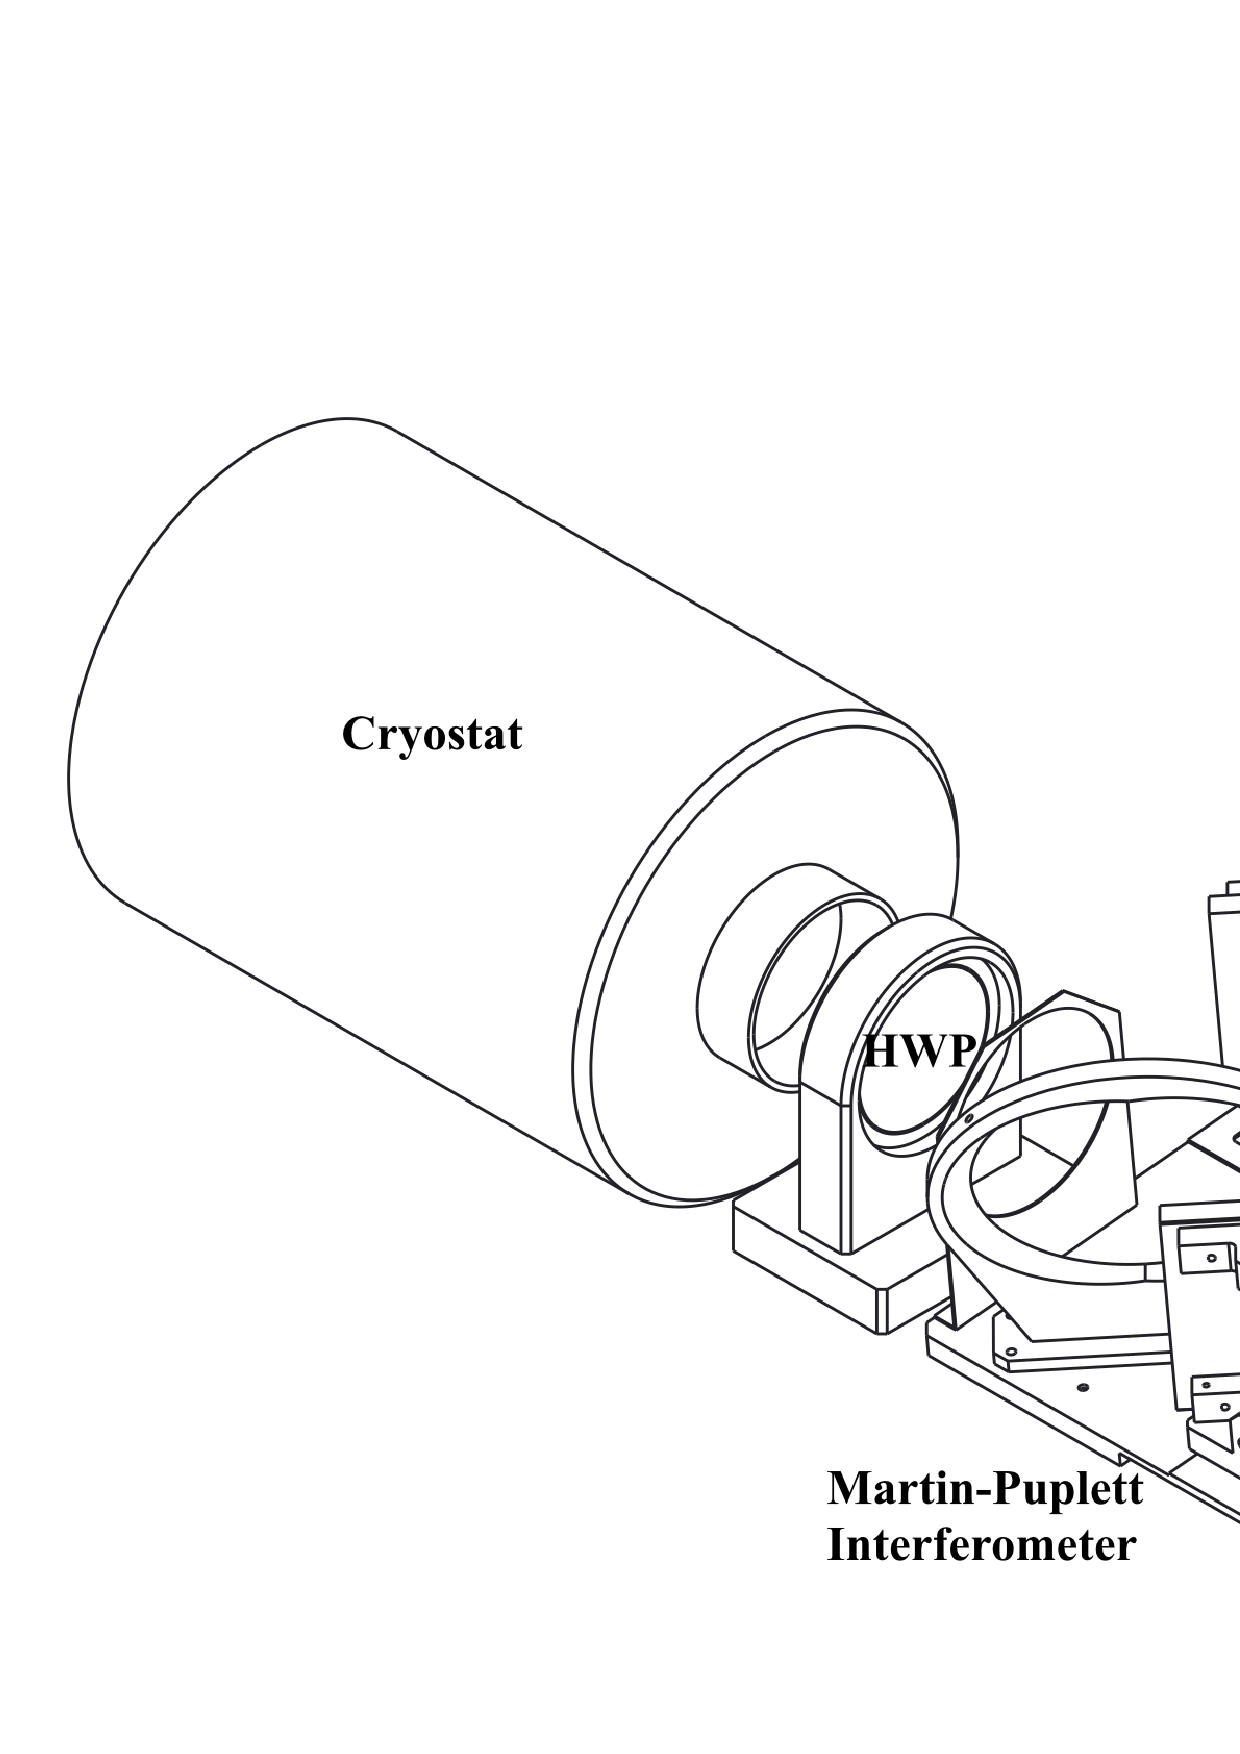
\includegraphics[width=7cm, keepaspectratio]{figures/Lab_test_config}
    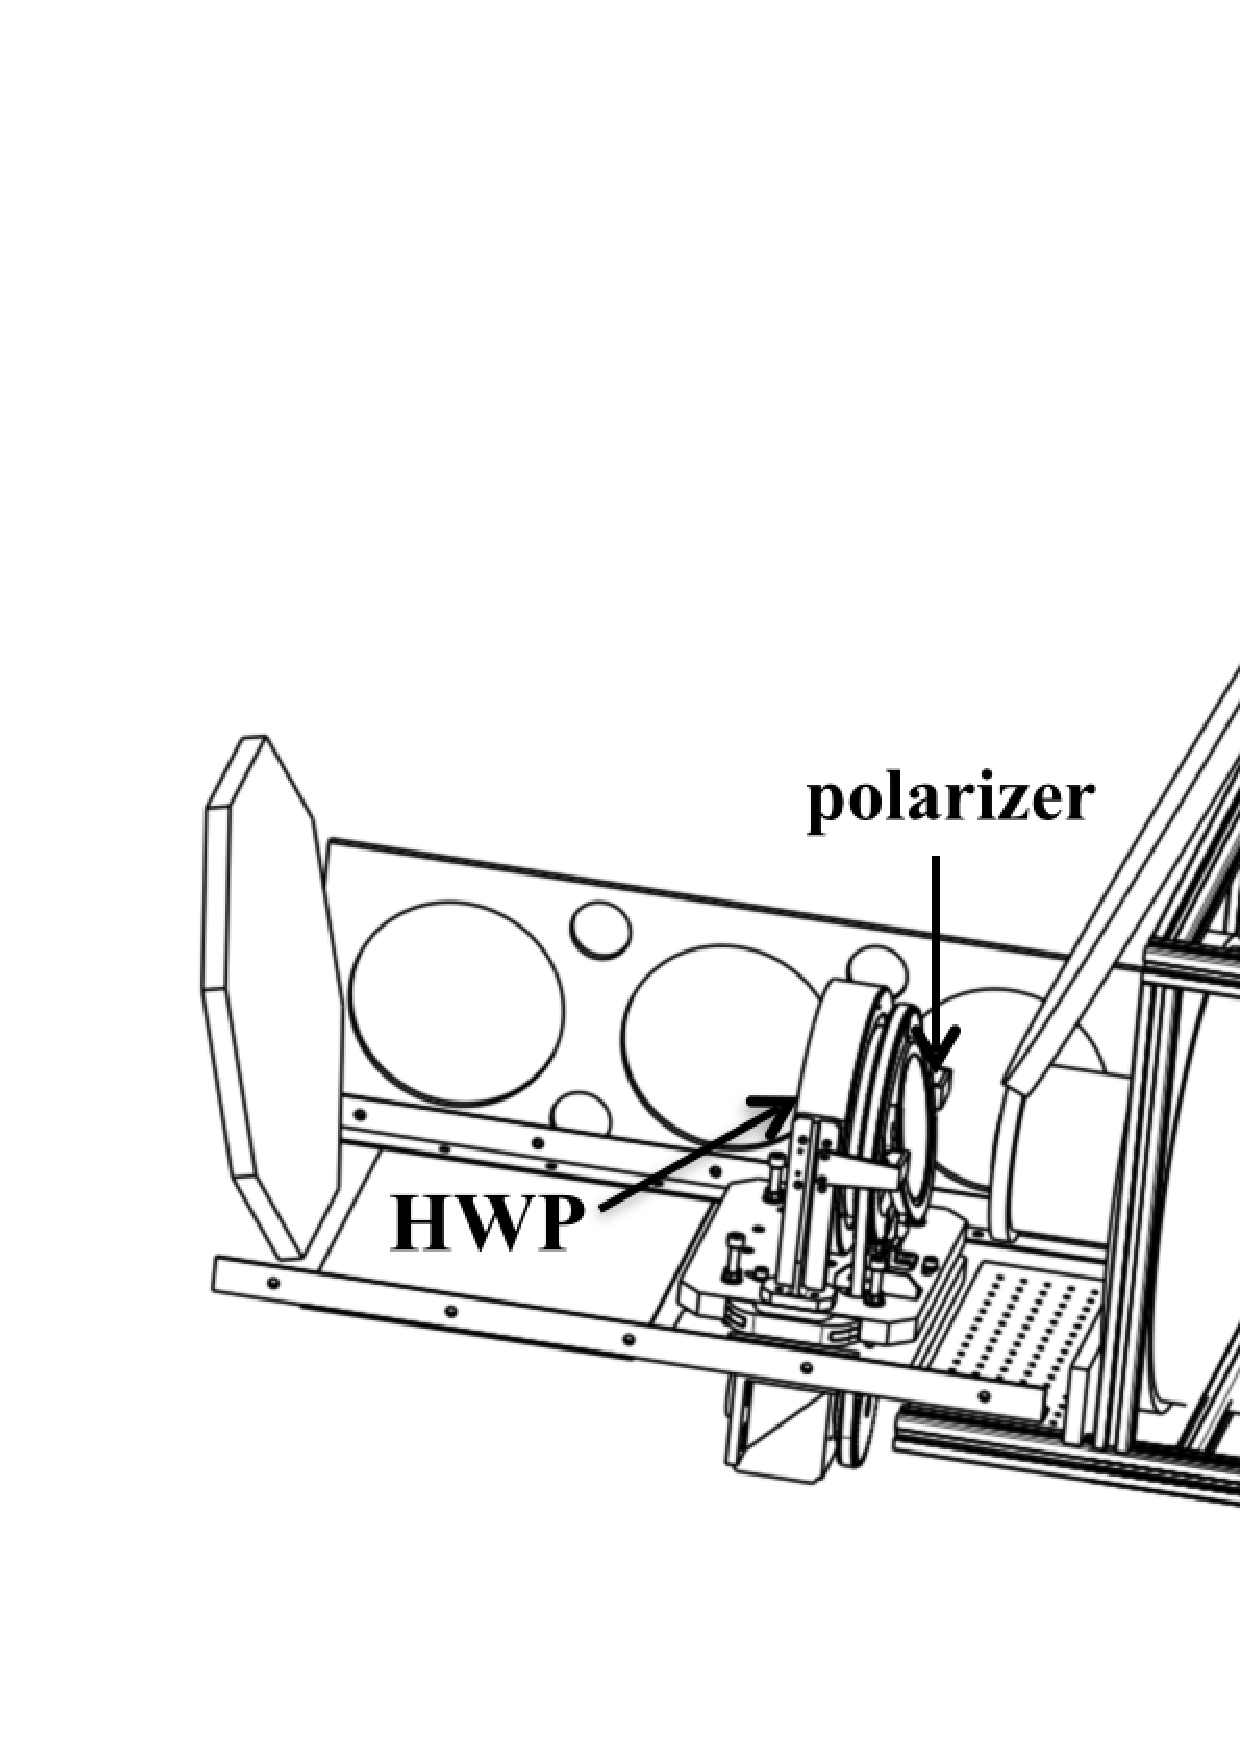
\includegraphics[width=7cm, keepaspectratio]{figures/setup_polar_telescope}

    \caption{Left: Laboratory instrumental setup. From left to right,
      the \nika\ cryostat, the HWP in a fixed position and a Martin-Puplett
      interferometer. Right: Instrumental setup for polarization measurements at
      the telescope. From left to right the last mirror of the telescope optics,
      the achromatic HWP mounted in the step motor, and the polarizer tilted by
      $\sim$ 10 degrees and the \nika\ cryostat. \label{polarsetup}}
  \end{center}
\end{figure*}

%\begin{figure}
% \begin{center}
%   \includegraphics[width=6cm, keepaspectratio]{figures/SETUP.pdf}
%    \caption{ Laboratory instrumental setup. From left to right,
%     the {\it NIKA} cryostat, the HWP in a fixed position and a Martin-Puplett
%      interferometer.}
%    \label{fig:setup_lab}
%  \end{center}
%\end{figure}

The polarisation setup of the \nika\ camera consisted of a continuously rotating HWP and an analyser, at room temperature,
facing the \nika\ camera window. 

The Hilbert geometry \citep{roesch} of the \nika\ LEKIDS was specifically optimised for intensity observations 
and as a consequence \nika\ LEKIDs were not sensitive to polarisation. Therefore, for polarisation observations an analyser was placed 
after the HWP at a distance of 6 cm of the cryostat window as shown in the two configurations of Figure~\ref{polarsetup}. The analyser,
consisting of a lithographic kapton coper polarimeter, was 10 degrees tilted with respect to the optical axis to avoid standing waves with the cold optical filters
inside the cryostat. 
%Experiments such as Planck
%\citep{planck_mission}, BICEP \citep{bicep}, ACTPol \citep{ACTPOL}, QUaD \citep{QUAD}, QUIET \citep{QUIET}, QUIJOTE \citep{QUIJOTE},  rotate
%the instrument w.r.t. the sky to vary $\psi$ and derive $I$, $Q$ and
%$U$. Experiments such as PILOT \citep{PILOT}, SPIDER \citep{SPIDER}, 
%use a HWP before an analyser to rotate $Q$ and $U$ while maintaining the payload
%attitude and so $\psi$ fixed. While these projects 
%maintain/s the HWP fixed observations and rotate it only between scans, in NIKA,
%like in EBEX \citep{ebex}, POLARBEAR \citep{polarbear}, BLASTPol \citep{BLASTPol}, we rotate it continuously. 
 
%In order to take in account the optical requirements at the telescope, the
%polarizer is mounted at a distance of 6 $cm$ from the HWP with its substrate
%plane at 10 degrees with the optical axis to avoid standing waves with the cold
%optical filters inside the cryostat.
The HWP was placed before the analyser by sharing the same holder. 
We used a hot-pressed metal mesh HWP designed and built at Cardiff University by \cite{pisano}.
The HWP was especially designed to allow approximately constant phase shift of the transmitted radiation over
a broad spectral band including the two \nika\ bands. A two-layer broadband anti-reflection coating was
added to the HWP to maximise the transmission across the band.
%and it has beent also hot-pressed on the front and back surfaces of the assembled plate.
The HWP was mounted into a mechanical modulator actioned by a stepper motor synchronously controlled by the \nika\
acquisition system. The power of the motor was chosen so that a typical stable rotation frequency of 5 Hz could
be achieved during observational campaigns of at least one week. We have chosen a
Sanyo Denki 103H8221-5141, which is a 2-phase stepping motor. 

The combined action of the continuously rotating HWP and the analyser leads to a modulation of 
the input linear polarisation at four times the mechanical rotation frequency, $\omega_{\rm rot}$. Thus,
letting aside calibration and system imperfections each LEKID
in the focal plane measures the following combination of the three Stokes parameters
\begin{equation}
m = I + Q \cos\left[ 2 \psi(t) + 4 \omega_P t) + U \sin ( 2\psi(t) + 4 \omega_P t\right].
\label{photoequ}
\end{equation}
{\nico Not
  sure we should restrict to Nasmyth here or be more general and refer to the x
  axis of the ref. frame to include the sky ref. frame}
$\psi$ is the angle between the analyser and the horizontal axis of the
polarization reference frame, which was set perpendicular to the light
propagation direction in the cabin Nasmyth reference frame. {\nico
  $\omega_P=2\pi \nu_P$ where $\nu_P$ is the rotation frequency of the HWP.}


% \nika~LEKIDs
%are sensitive to both polarizations and the polarizer placed behind the HWP
%plays the role of an analyser. It is rotated at constant pace by a stepper motor
%({\color{red} give a bit more details on this rotator...}
  
%%%\begin{figure}[h!]
%%\begin{figure}
%% \begin{center}
%%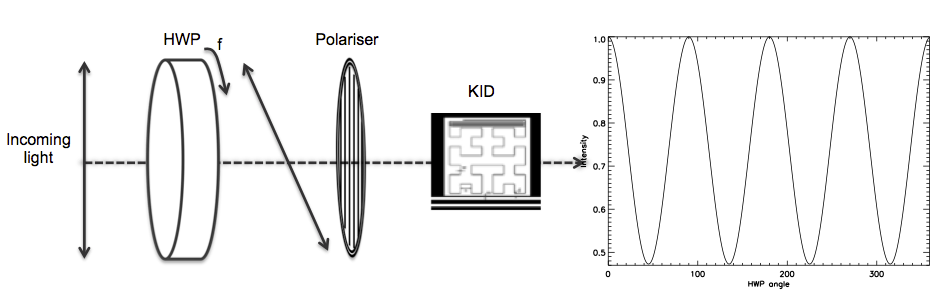
\includegraphics[width=8.5cm, , keepaspectratio]{figures/setup_polar.png}
%%\caption{ Observational polarimeter scheme. From left to right we
%%  observe the rotating HWP, the polarizer and the {\it NIKA} cryostat containing
%%  the arrays of LEKID detectors.}
%%\label{fig:setup_polar}
%%\end{center}
%%\end{figure}

\section{Laboratory characterization of the polarimetric module}
\label{sec:lab_characterization}

%\begin{figure}[h!]


%{\color{red}
%\begin{itemize}
%\item[-] {\color{green} the ``cryostat'' used in these lab tests actually was \nika, right
%  ? let's mention it then and rephrase the sentence. {\color{cyan} non, it was not.}}
%\item[-] need to add a word on what was done in Cardiff and
%  why we do or do not report on this here.
%\item[-] Need to justify what previous experience allows us to assume that the
%  polarizer is perfect.
%\item[-] I don't understand why we talk about distortion of the bandpass with
%  the HWP rotation ? Do you mean ``attenuation'' instead ?
%\item[-] {\bf We need to explicit an equation to explain why it's a 45 deg
%  rotation that separates max and min transmissions (add formula somewhere somehow)}
%\item[-] I've removed the mention to the ``linear shift'' between the two bands
%  because it's not shown on any plot and not dicussed. If we do have sthg to say
%  about this, we should develop more. We should definitely say and show that the
%  HWP is achromatic.
%\end{itemize}
%}
We start this section by introducing the main parameters used in the characterisation 
of the \nika\ HWP. The Mueller matrix of a general realistic HWP can be written as

\begin{strip}
 %\begin{widetext}
  \begin{eqnarray} \label{equ.HWP}
%    \begin{split}
      M_{HWP}=\frac{1}{2} \left(\begin{array}{lll} \\
        \alpha^2+\beta^2              & (\alpha^2-\beta^2)\cos2\theta & (\alpha^2-\beta^2)\sin2\theta \\
        (\alpha^2-\beta^2)\cos2\theta & (\alpha^2+\beta^2)\cos^22\theta +
        2\alpha\beta\sin^22\theta\cos\phi &
        (\alpha^2+\beta^2-2\alpha\beta\cos\phi)\cos2\theta\sin2\theta \\
        (\alpha^2-\beta^2)\sin2\theta &
        (\alpha^2+\beta^2-2\alpha\beta\cos\phi)\cos2\theta\sin2\theta &
        (\alpha^2+\beta^2)\sin^22\theta + 2\alpha\beta\cos^22\theta\cos\phi
%        \label{eq:mueller_mat}
      \end{array}\right)
   % \end{split}
  \end{eqnarray}

%\end{widetext}
\end{strip}

\noindent The $\alpha$ and $\beta$ coefficients represent the normalised transmission coefficients on the ordinary and extraordinary axes of the HWP. 
The HWP phase shift angle between the ordinary and extraordinary axes is noted as $\phi$.  $\theta$ represents the angle of the 
HWP ordinary and extraordinary axes with respect to the polarisation reference frame. \\

A first characterisation of the properties of the \nika\ HWP was carried out after fabrication
at Cardiff University. In particular the HWP phase shift angle, $\phi$, was measured over the full
bandwidth from 100 to 350~GHz as shown in the top panel of Figure~\ref{fig:spectre}. \\

%pour trouver maximum on prend trois spectre dans la region maximale et puis on prend le plus haut 
%{\color{red} \bf alpha et beta : 8 spectres a difference angles
%nombre de pas MPI: 80
% spectral resolution of about 3.5GHz (about 44 mm of excursion of the roof mirror)
%temps de me sure: 9.16 min
%characterisation axes optique ->  mesures int�gres sur la bande et on a cherche le maximum et le minimum}

Furthermore, in order to estimate the performance of the whole polarization chain,
we performed laboratory measurements of the system transmission. 
We used a polarising Martin Puplett Fourier Transform Spectrometer (MPFTS) to characterize the spectral transmission of the system. 
The MPFTS produces the difference between the power of two input polarised beams that come from two
black bodies at different temperatures (ambient eccosorb and warmed eccosorb) modulated by a rotating wire-grid polarizer.
An array of LEKIDs was placed facing the MPFTS inside a \nika\ type dilution cryostat, which cools down the optics, the analyser and the LEKIDs to 100 mK.
The analyser consists of a wired-grid and it will be considered as ideal in the following.
A schematic view of the instrumental setup is shown on the left panel of Figure~\ref{polarsetup}.

We have performed a total of eight independent measurements by varying the angle of the \nika\ HWP axis with respect to the optical axis.
For each transmission measurement the HWP was kept fixed during data taking. We achieved a spectral resolution of about 3.5 GHz, 
which corresponds to about a 44 mm excursion of the roof mirror of the MPFTS. We covered the bandwidth of
interest by considering a total of 80 steps by transmission measurement for total of 9 minutes of integration time. 
As the MPFTS polariser and the analyser transmission axis were set perpendicularly to each other,
prior to any measurement we rotated the \nika\ HWP to find a zero point initial position, which maximised the measured LEKID signal. 

%As far as the polarization module
%is concerned, we assume an ideal polarizer {\color{red} say briefly why} and we
%focus only on the characterization of the HWP parameters. 

By rotating the HWP for each measurement we rotated the polarisation of the MPFTS output signal. 
As the analyser was kept at fixed position, this induced an attenuation of  the signal measured by the LEKIDs.  
This can be observed in the bottom panel of Figure~\ref{fig:spectre} where we present
the measured transmission as a function of frequency for four HWP positions going
from the maximum (black solid line) to the minimum of transmission (dashed solid line) spectra.
As expected the relative HWP angle between the maximum and minimum transmission is about
45 degrees.
%When the HWP
%aligns the polarization with the analyser, we have maximum transmission ($46.8
%\pm 1.8^{\circ}$), when it aligns it in the orthogonal direction, we have
%minimum transmission ($86.4\pm1.8^\circ$). The nearly $45^\circ$ difference
%between these two HWP positions agrees with
%Eq.~(\ref{eq:hwp_and_polarizer}). Note that we cannot expect zero transmission
%because of the wide band of the instrument ({\color{red} Please confirm this or
%  give explanations why we do not measure strictly 45 deg within error bars :)
%  Actually, the absolute error is not 1.8 deg but 3.6 deg, which is now
%  compatible with the 5 deg difference between 45 theoretical and 40 measured,
 % but we need to make clear in the paper, that the stepper motor is very well
 % controlled and that the error on each individual angle is much less than 3.6
%  deg.}. 

We used previous transmission spectrum measurements to determine
the $\alpha$ and $\beta$ transmission coefficients describing the HWP.
Taking as a reference the maximum transmission spectrum described above,
we fit for the other transmission spectra taken at different angles of the HWP
with respect to the reference polarisation axes. We assumed the 
HWP model in Equation~\ref{equ.HWP} and accounted for the analyser facing
the LEKID array. The phase shift angle, $\phi$, was set to the values per frequency measured
at Cardiff University and presented above.
%birefringent axes. $\theta$ is the angle of the incident polarization with
%respect to the reference frame defined by these axes and {$\phi$} is the phase
%shift introduced by the plate between the two orthogonal polarizations. $\phi$
%is a vector of values found during the simulations carried out by Cardiff group
%when the HWP was manufactured in order to optimize the trasmission of the
%polarized light. 
Notice that as we are using the maximum transmission
spectrum as a template we are not sensitive to an overall attenuation amplitude.
Therefore, to simplify the procedure we fixed $\alpha$ to one and we
only fitted for $\beta$. Using a least square minimisation we find $\beta = 0.994\pm0.005$ at 1.25
mm and $\beta = 0.924\pm0.005$ at 2 mm. The best fit models obtained for each position
of the HWP are plotted in red in Figure~\ref{fig:spectre}.

Defining the polarization efficiency as $\rho_{pol} = (1-2\gamma)/2$ where $\gamma = \frac{\alpha \beta
  \cos(\phi)}{\alpha^2 + \beta^2}$ we find $\rho_{\rm pol} = 0.994 \pm 0.01$ at
1.25 mm and $0.986 \pm 0.01$ at 2 mm. These values are accounted for in the
final absolute calibration of our polarization maps. Finally, as a consequence of the  small difference observed between
the $\alpha$ and $\beta$ transmission coefficients we expect the modulation the incoming intensity and polarization around the second
harmonic of the HWP rotation. However, as presented in Sect.~\ref{se:demod_mapmaking}, we are not sensitive to this effect in the
final maps as it is accounted for in the data processing.

%% of the for each wavelength due to the linear relation
%% between the phase shift and the wavelength. This effect is expected to be quite
%% weak because the HWP is achromatic \citep{moncelsi2014}. First we measured a
%% spectrum with the HWP aligned to its ordinary axis. This corresponds to the
%% maximum signal in which we expect to have no distortion {\color{red} see
%%   comment} of the {\it NIKA}
%% bandpass, as measured in intensity \citep{catalano2014}. This is taken as a
%% reference spectrum. Rotating the HWP we found an attenuation as shown in
%% fig. \ref{fig:spectre}, here the maximum transmission is represented by the
%% spectrum at about 46.8$^{\circ}$ $\pm$ 1.8$^{\circ}$ with respect to the HWP
%% zero.

% The polarized transmission is therefore of $\sim$ 100\% in the {\it NIKA} band
% frequency with a polarized transmission loss of 0.6 $\%$ in the 1mm channel and
% of 1.4$\%$ in the 2mm channel.
 
%In the 1mm channel the polarization loss is very low so we consider to work with
%an ideal HWP assuming the $\rho_{pol}$ = 1 in the following data reduction
%analysis. In the 2mm channel we take into account for the coefficient
%$\rho_{pol}$ in the calibration factor.

\begin{figure}[t!]
  \begin{center}
   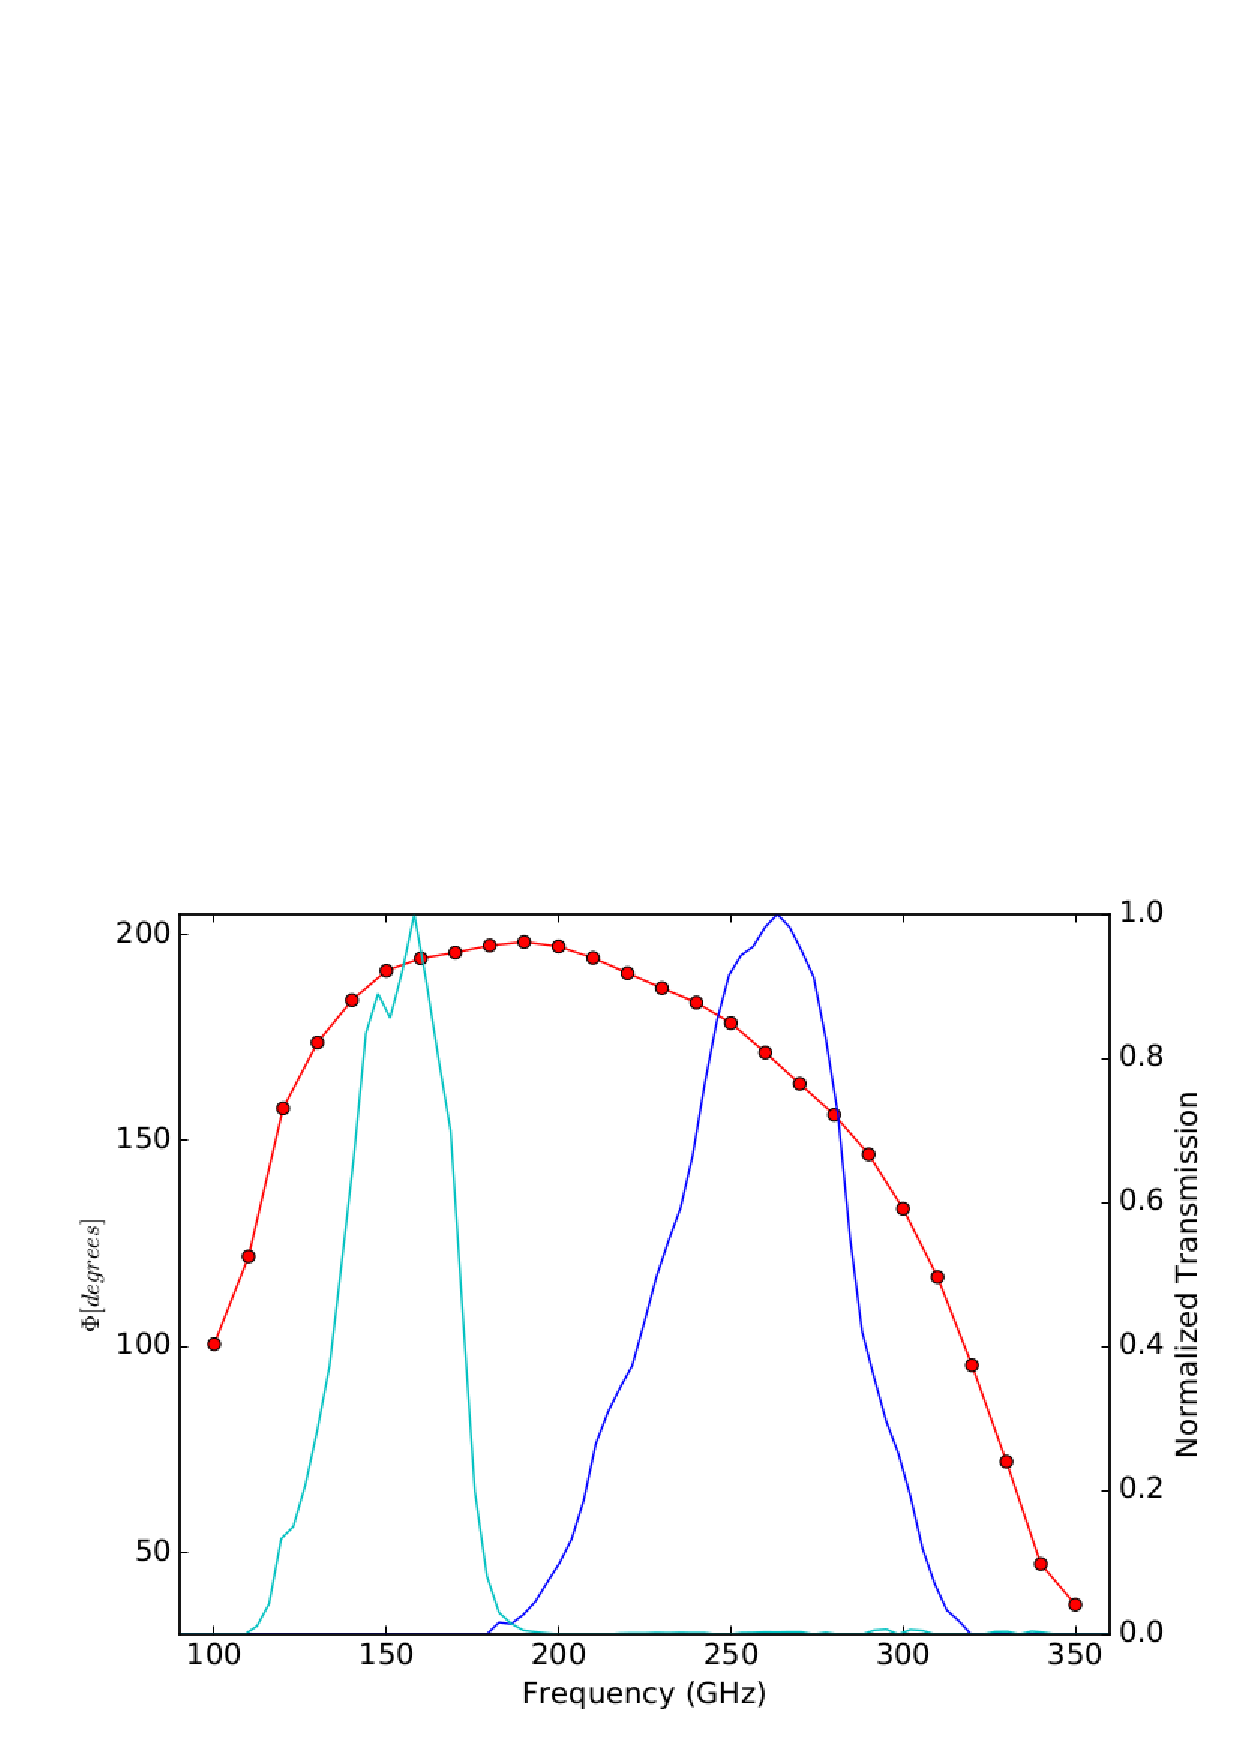
\includegraphics[width=6.5cm, keepaspectratio]{figures/phase_shift_angle}
   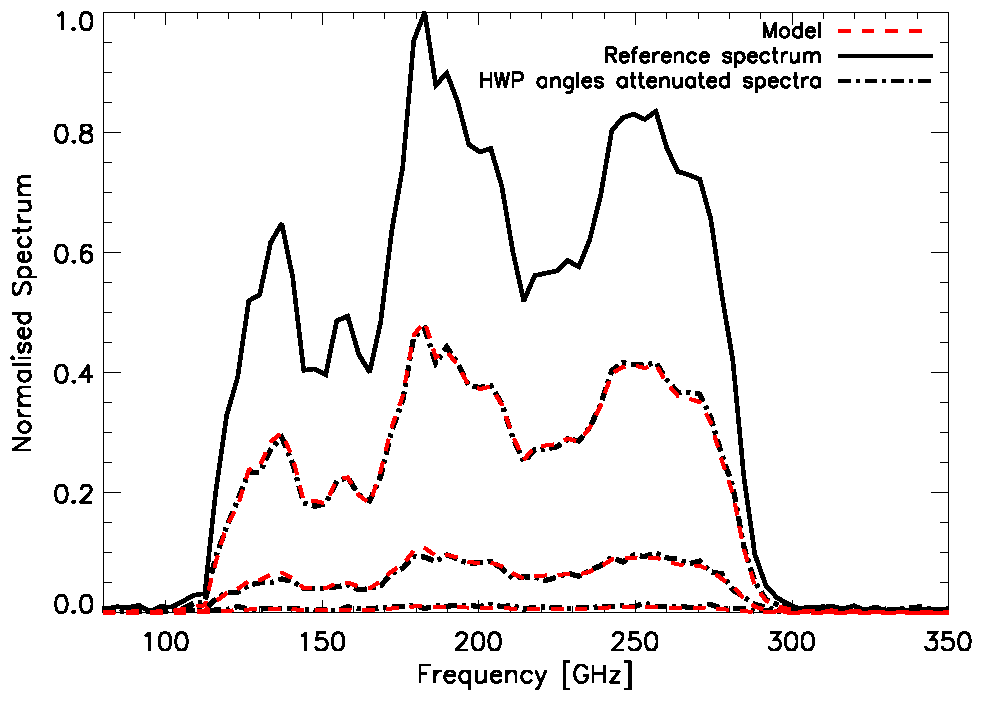
\includegraphics[width=6.5cm, keepaspectratio]{figures/spectre}
    \caption{Top: Phase shift angle as a function of frequency for the \nika\ HWP. Bottom: 
    Spectral transmission of the \nika\ HWP at different angles with respect to the optical axis.
    The red curve corresponds to the best-fit model for the intermediate angle data.}
    
%    Maximum transmission at an angle of 46.8$^{\circ}$
 %    respect to the HWP zero and attenuated spectra at 72$^{\circ}$,
%      79$^{\circ}$, 86.4$^{\circ}$ (top curve to bottom curve). For example, the
 %   model (red dotted line) fits the spectrum at an angle of 72$^{\circ}$.}
    \label{fig:spectre}
  \end{center}
\end{figure}
		

%\section{Observation strategy for polarization measurements}
\section{Data analysis and derivation of Stokes parameters maps}
\label{data_analysis}

We here describe the specificities of \nika's polarization modulation strategy
and data analysis. We start by giving more details on the fast and continuous
rotation of the HWP and how it impacts the signal. We then present specific
systematics associated to the rotating HWP and the optics, and how we cope with
them. 
%We postpone the determination of the absolute polarization angle on the
%sky and of the absolute calibraiton to the following section.

 \begin{figure*}
  \begin{center}
  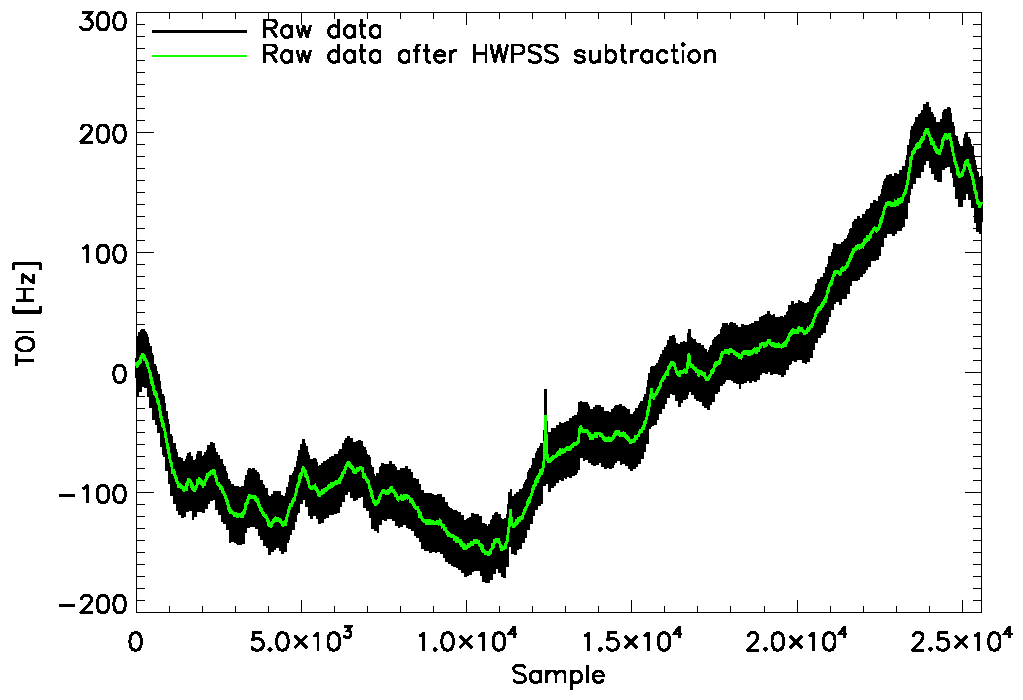
\includegraphics[%
  width=9cm, keepaspectratio]{figures/TOI}
  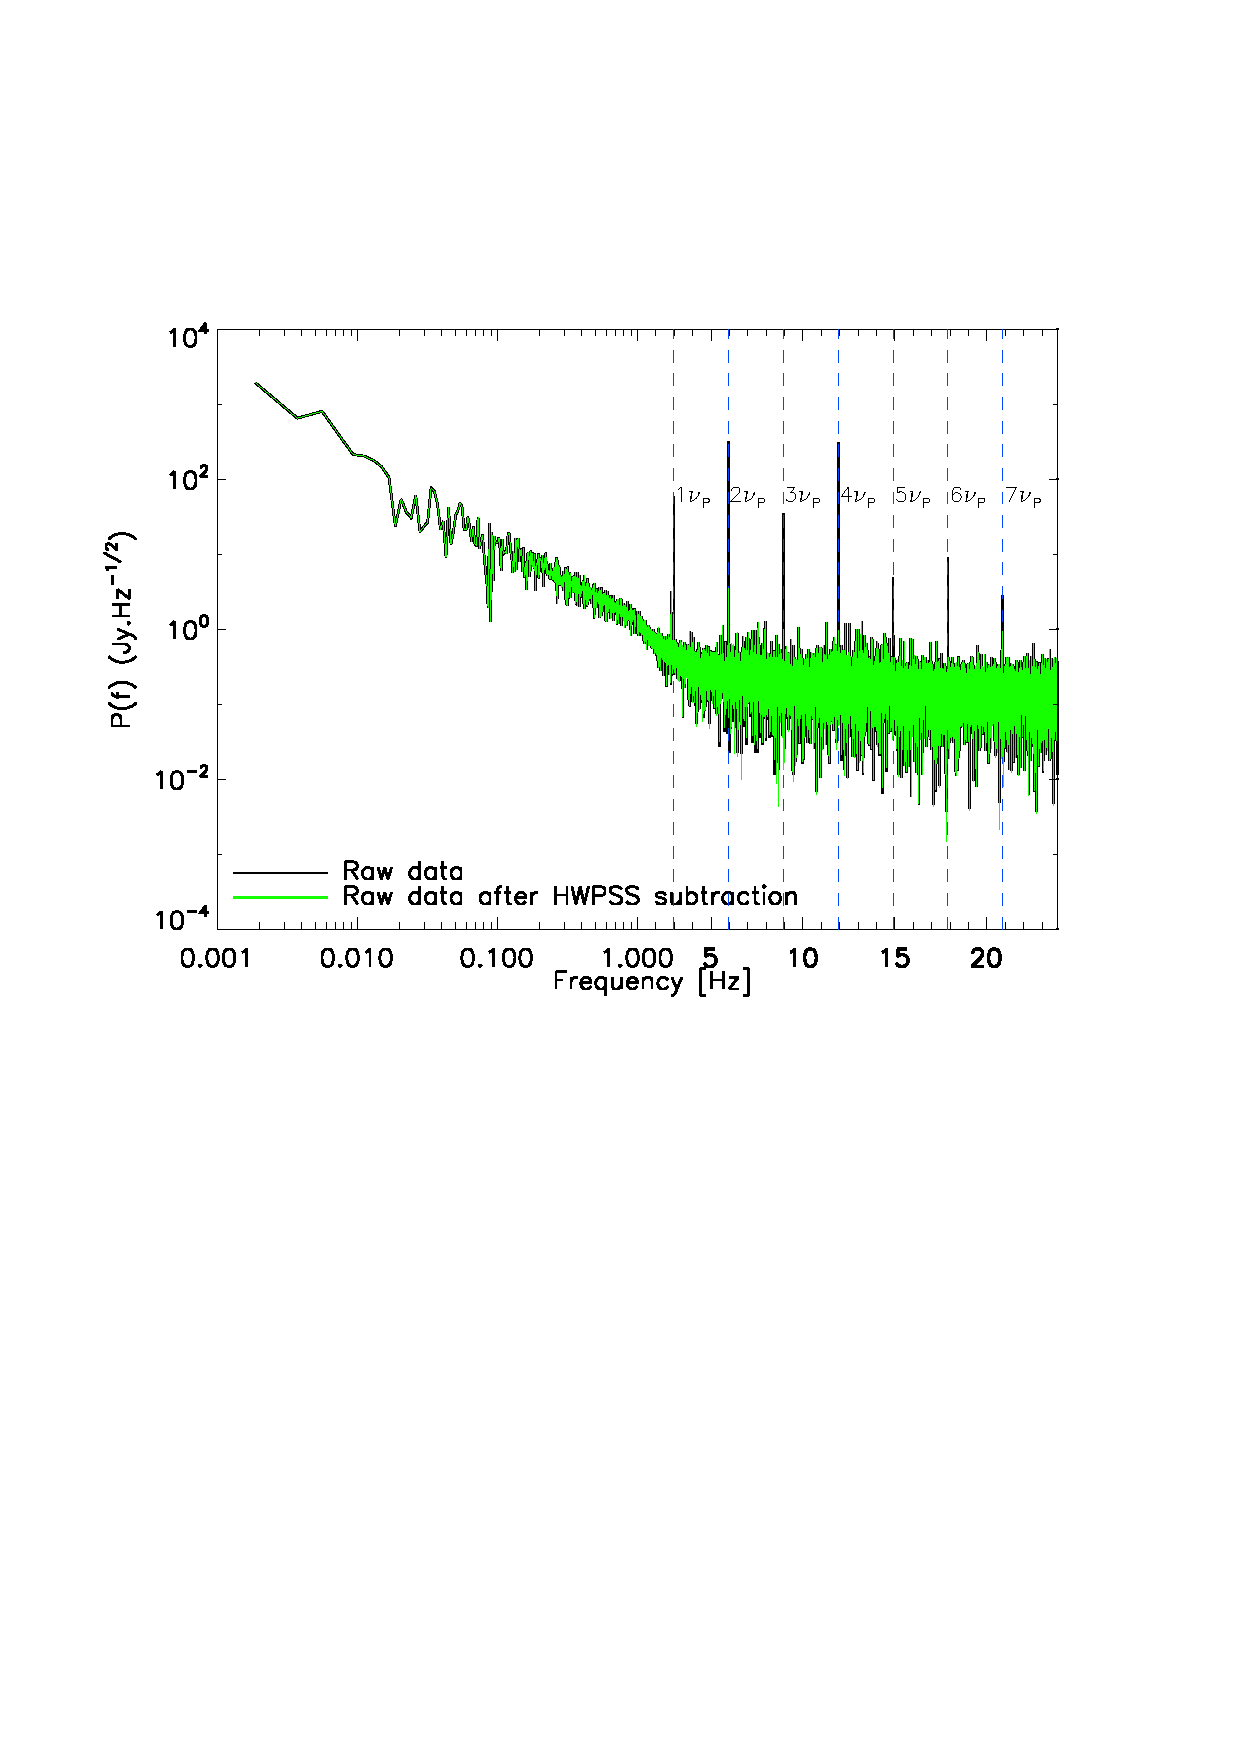
\includegraphics[%
  width=8.5cm, keepaspectratio]{figures/spectre_I_fit}
 
 % 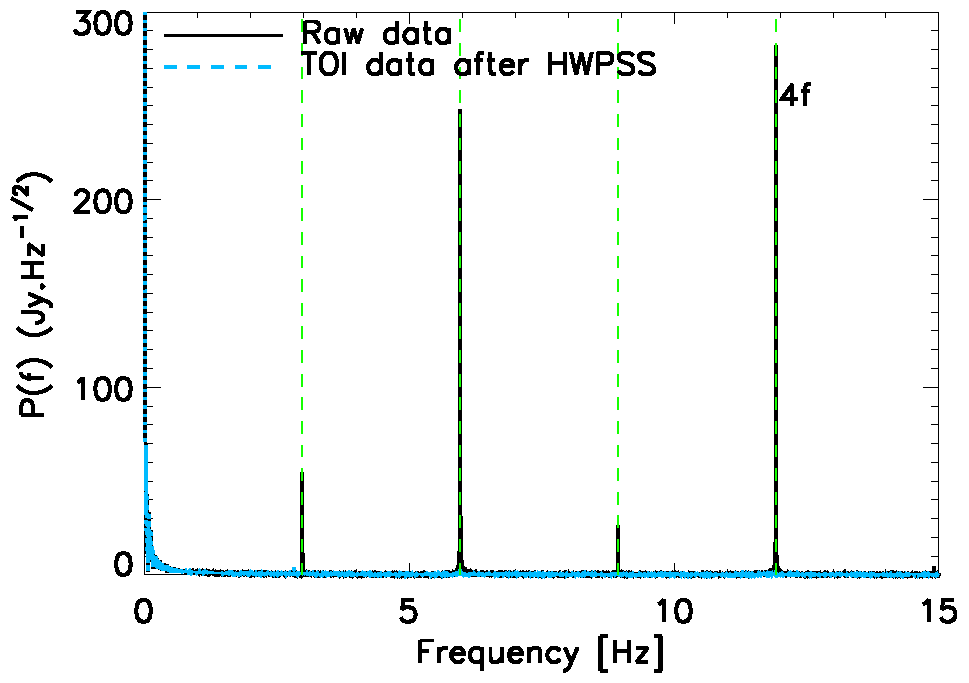
\includegraphics[%
 % width=5.3cm, keepaspectratio]{figures/Ps_I_zoom_nolog_I.pdf}
  % 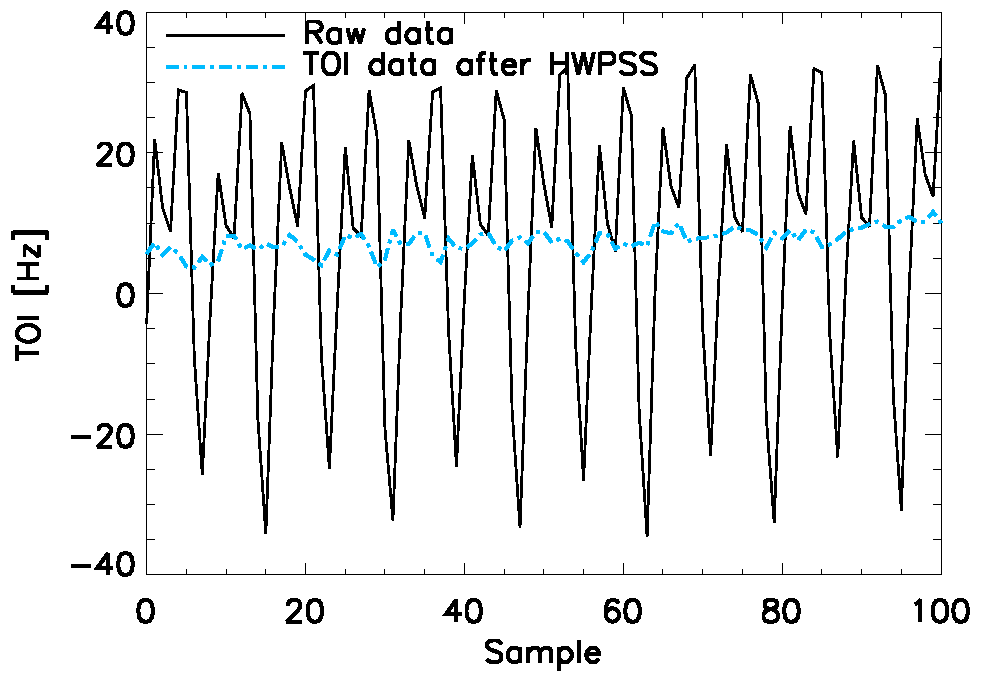
\includegraphics[%	
 % width=5.3cm ,keepaspectratio]{figures/timeline_zoom_I}
 \caption{Left panel: Time Ordered Information (TOI) for an observation of Orion
   OMC-1 and a KID $k$. Raw data in black, subtracted data for the HWPSS in
   green. Right panel: Power Spectrum for the raw TOI before subtraction for the
   HWPSS (black) and after (green).{\nico redo the power spectrum plot in
     log/lin x axis (nico). There's an xyouts, ``4f'' on the power spectrum plot that
     must be harmonized with the simulated power spectrum and its ``$4\nu_P$'' and
     the ``$1/f$'' fit on fig.~\ref{spectre_iqu} (Nico)}}
  \label{toi_i}
   \end{center}
   \end{figure*}
   
 \begin{figure*}
   \begin{center}
     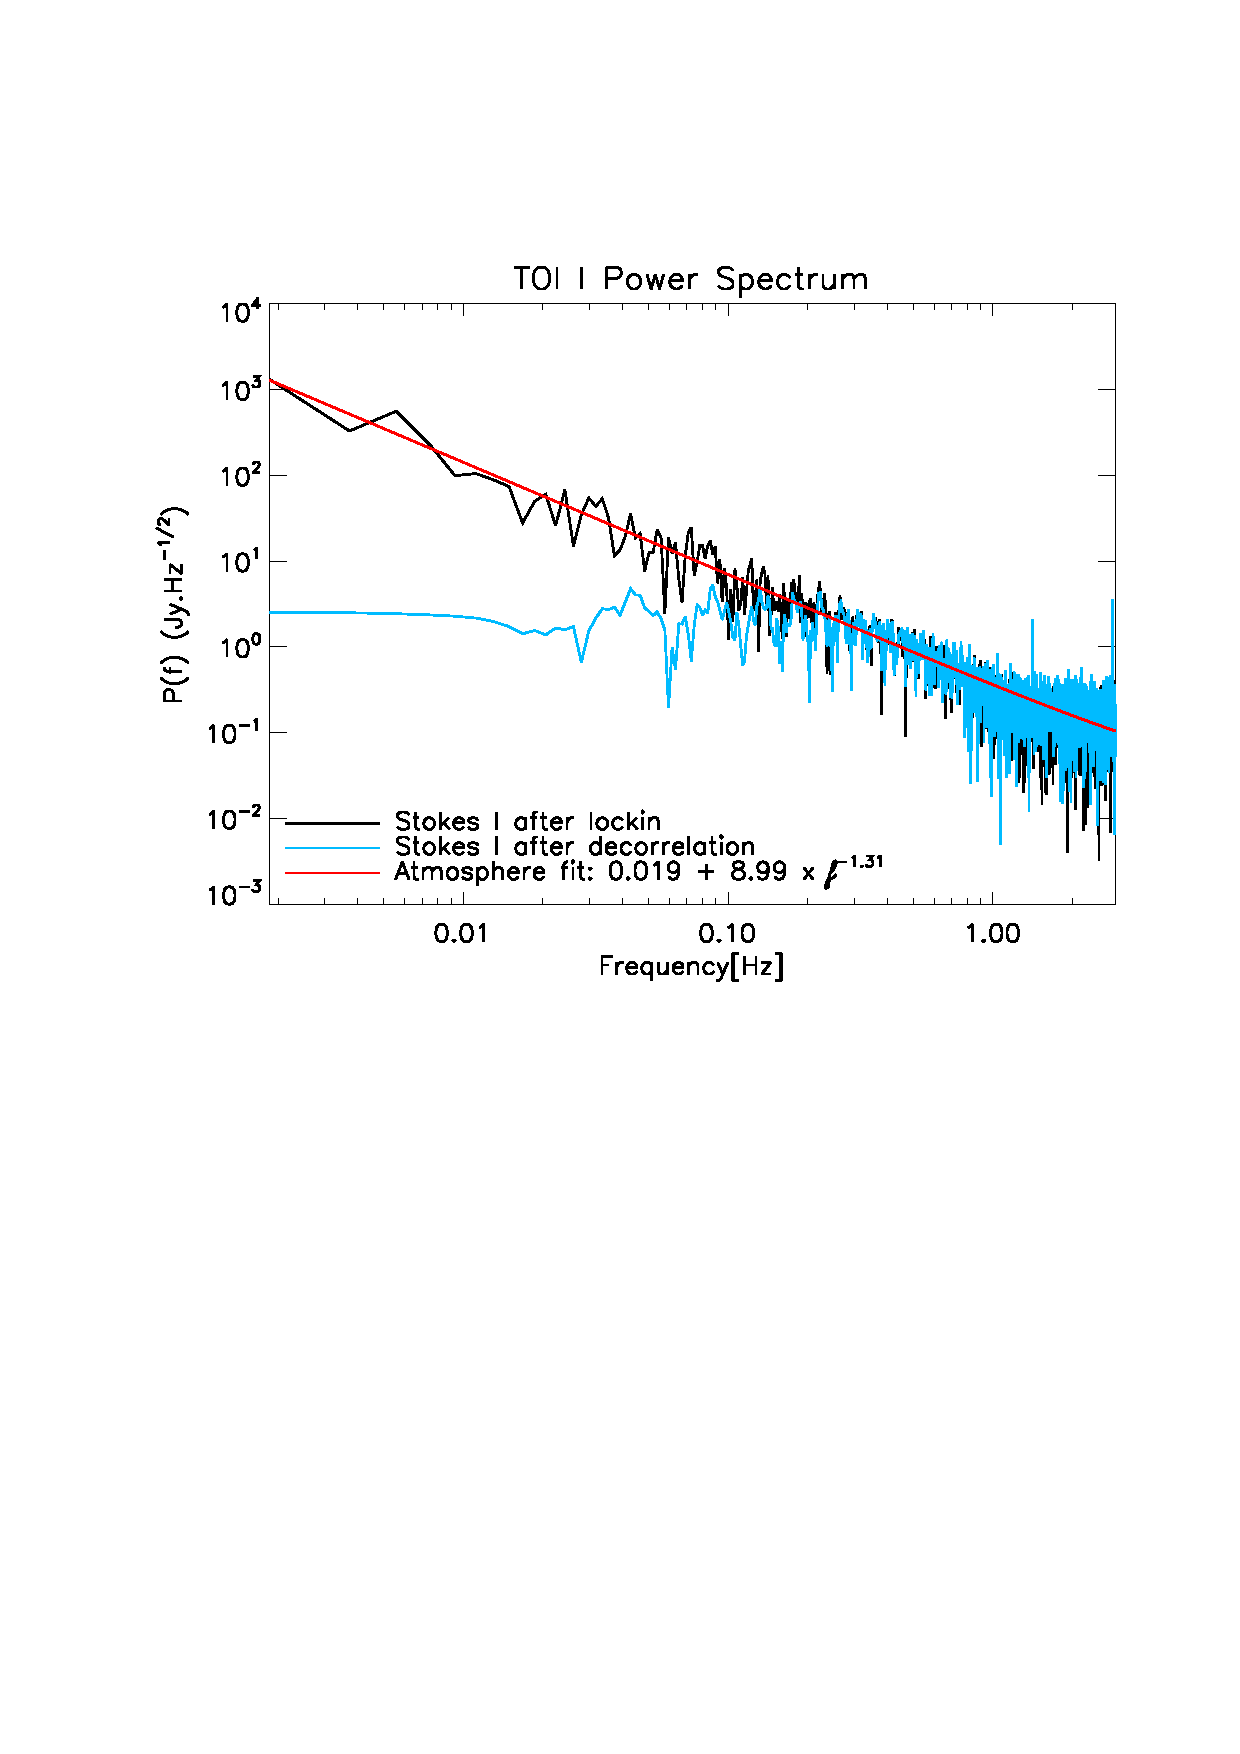
\includegraphics[%
       width=5.8cm,keepaspectratio]{figures/spectre_I_fit_decor}
     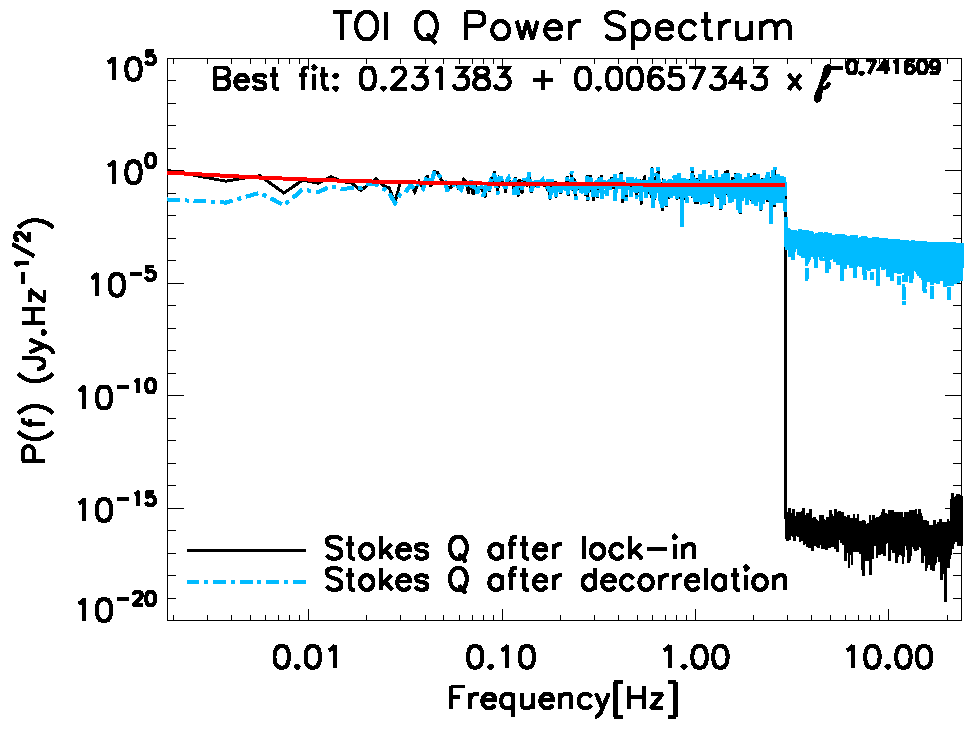
\includegraphics[%	
       width=6cm,keepaspectratio]{figures/spectre_Q_fit}
     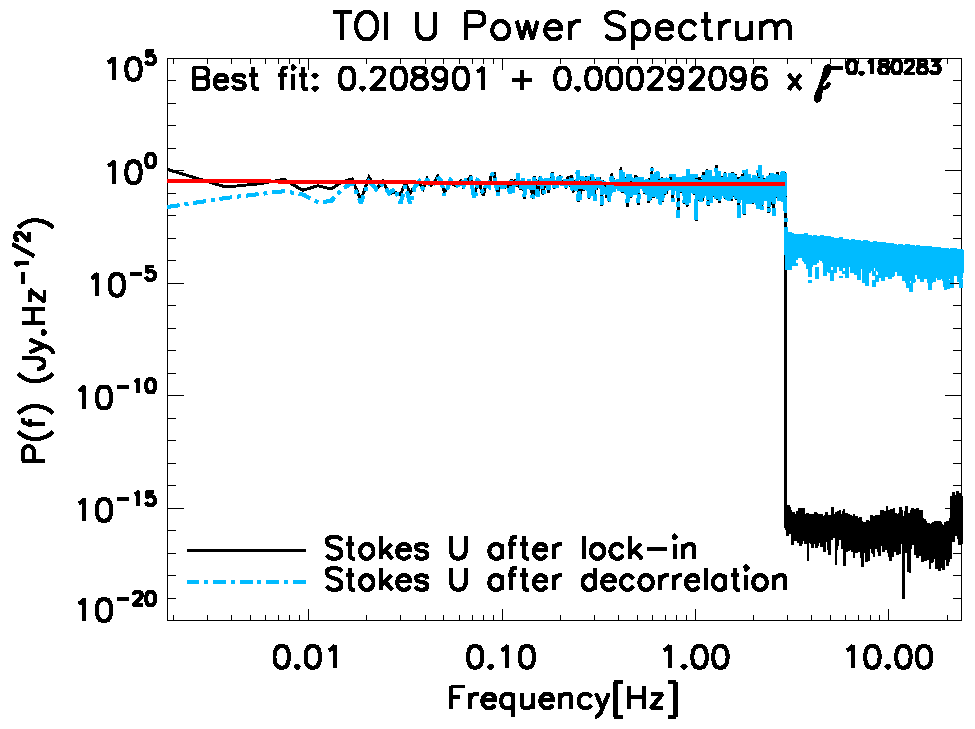
\includegraphics[%	
       width=6cm,keepaspectratio]{figures/spectre_U_fit}
     \caption{From left to right: power spectra of the Stokes vector $I$, $Q$,
       $U$. The $I$, $Q$, $U$ timelines (black line) are obtained thanks to the
       lock-in procedure, a bandpass filter is applied to reject any high
       frequency noise; in blue we show the $I$, $Q$, $U$ timelines obtained
       after decorrelation.{\nico stick plots together and truncate fit
         coefficients. The high frequency ``blue'' noise is higher than the high
         frequency ``black'' noise: this is due to the construction of the
         median common mode during the decorrelation. We must be careful on how
         we present this plot and justify this. (Nico)}}
     \label{spectre_iqu}
   \end{center}
 \end{figure*}
 
{\nico 
\subsection{Polarization modulation with a continuously rotating HWP}
\label{se:lockin}

%: a scan in azimuth at constant elevation and constant speed
%$v$, an elevation step smaller than the beam FWHM, another azimuth scan at this
%new elevation, this sequence being repeated until we have scanned the desired
%sky area. In such a case, the point source signal appears in time domain at
We recall here the main lines guiding polarization modulation by a continously
rotating HWP and its subsequent data analysis. For the sake of clarity, we
consider the case of single polarized point sources, observed under a classical
raster scan strategy at speed $\dot{\alpha}$. This type of scan being
pseudo-periodical, the Fourier transform of a TOI shows peaks at harmonics of
the scanning frequency, each peak containing the sum of the unpolarized and
polarized fluxes of the source. These peaks are then damped by the instrument
resolution at high frequency: the beam cut off at high spatial resolution turns
into high temporal frequencies cutoff with typical gaussian width $FWHM_\nu =
\dot{\alpha}/2\pi FWHM$. This beam cutoff defines the signal band. According to
eq.~(\ref{photoequ}), when we rotate a HWP in front of an analyser, the
polarized fraction of the signal is modulated at four times the mechanical
rotation frequency of the HWP. This shifts the polarized content of the signal
at higher frequencies and recenters the signal band around the fourth harmonic
of the mechanical rotation of the HWP (Fig.~\ref{fig:toi_simu}-top). It is then
clear, that a lowpass filter applied to the data above the beam cutoff and below
the polarization signal band will preserve the unpolarized signal band while
rejecting the polarized content and high frequency noise. We will refer to this
type of timelines as ``pure-$I$'' timelines in the following. To recover the
polarization Stokes parameters $Q$ and $U$, we use a procedure pioneered by
\cite{johnson2007}. We build two reference signals $\cos(2\psi(t) + 4\omega_Pt)$
and $\sin(2\psi(t) + 4\omega_Pt)$. We multiply our timelines by these reference
signals and according to eq.~(\ref{photoequ}) obtain e.g. $Q/2 +
I\cos[2\psi(t)+4\omega_Pt] +...$ $Q$ and $U$ terms around the 8th harmonics of
the HWP rotation. We have thus ``demodulated'' the $Q$ content of the timeline
and brought it back at low frequencies, while rejecting the $U$ and $I$ content
at high frequencies. A low pass above the beam cutoff and below the tail of the
modulated intensity therefore provides a pure-$Q$ timeline
(Fig.~\ref{toi_simu}-bottom). The same goes for a multiplication by
$\sin\left[2\psi(t)+4\omega_Pt\right]$ to obtain a pure-$U$ timeline.

\begin{figure}
\includegraphics[width=1.\linewidth,keepaspectratio]{figures/toi_simu.eps}
\caption{Power spectrum of a simulated timeline for a polarized point source
  observed under a raster scan and polarizatin modulation by a continuously
  rotating HWP in front of an analyser. The raw timeline has its total intensity
  content highlighted in cyan and polarized content in green. The polarization
  signal band is centered on the fourth HWP harmonics while the intensity signal
  band lays at low frequencies. On the bottom plot, the timeline has been
  demodulated (see. Sect.~\ref{se:lockin}), half its $Q$ content has been put at
  low frequency while the $I$ content and the remaining polarized contents are
  shifted at frequencies higher than the signal band.}
\end{figure}
}


\subsection{Polarisation setup at the telescope and polarisation reference frame}
{\nico
The \nika\ polarisation setup at the telescope was similar to the one in the
laboratory as shown on the right panel of Figure~\ref{polarsetup}.  The HWP and
analyser were placed in the same mount facing the cryostat window in the optical
axis of the Nasmyth cabin. Thus, the polarisation reference frame was defined
perpendicularly to the optical axis in Nasmyth coordinates. As in the laboratory
case the analyser was slightly tilted (about 10 degrees) with respect to the HWP
to avoid standing waves. The HWP rotation speed is constrained by several
factors. Usual scanning speeds of the order of one arcmin/s or less, combine
with atmospheric variations into a $1/f$ like noise with knee frequency below
1~Hz. Electronics noise becomes subdominant above 1~Hz as well {\color{red}
  exact value TBC}. Rotating the HWP such that 4 times its rotation speed places
the polarization signal well above 1~Hz allows a natural rejection of these two
types of noise. If the rotation is also fast compared to the scanning speed and
the angular resolution, all the Stokes parameters for a given direction in the
sky can be derived quasi-simultaneously, thus rejecting further residual low
frequency drifts. Last, a fast rotation places parasitic signals at harmonics of
the rotation frequency outside the signal band (see sect.~\ref{se:hwpss} for
more details). On the other hand, a fast rotation sets tighter mechanical
constraints on the stepper motor and impose a faster data
acquisition. Accounting for all this, we chose to acquire data at 47.7~Hz,
rotate the HWP at 2.98~Hz and limit our scanning speed to 26~arcsec/s. This
provides 5 measures of $I$, $Q$ and $U$ per FWHM, well within the Nyquist limit,
even at a LEKID timeline level. The specific values of the data acquisition rate
and the HWP rotation are determined by our electronics and our will to have
synchronous HWP rotation and acquisition.

To project maps of the three Stokes parameters, we use the lockin procedure
described in Sect.~\ref{se:lockin} to build pure-$I$, pure-$Q$ and pure-$U$
timelines. We lowpass at 2.9~Hz which preserves the signal content up to -3dB
{\color{red} on est bien d'accord que -3dB ca veut bien dire $10^{-3}$ ?! ;-)} while
rejecting any remaining parasitic noise at the closest HWP harmonics. We then
coadd the timelines onto maps with inverse noise weighting. This is almost
equivalent to optimal map making given that the noise is very close to being
white in our polarization timelines (see Fig.~\ref{spectre_iqu}) {\color{red}
  Recheck this plot and its caption}.
}

%%  {\nico The HWP was continuously rotated at 2.98 Hz and the
%% data were sampled at 47.7 Hz (see below for more details)} that corresponds to
%% about twice the sampling frequency during intensity only observations. This
%% combination of sampling and HWP rotation frequency allows us to sample four
%% different positions of the HWP, which is equivalent to observe the incoming
%% polarisation at four independent angles{\nico on what time scale ? Need to talk
%%   about the constraints on the scanning speed as well}. This fast modulation
%% allows us to reconstruct the three Stokes parameters, I, Q and U independently
%% for each detector and to reduce significantly atmospheric contribution as
%% described below.
%% 
%% \subsection{Timelines demodulation and map making}
%% \label{se:demod_mapmaking}
%% 
%% %In order to extract the polarized signal from the unpolarized foreground we use
%% %the modulation/demodulation technique: by means of a polarization modulator, the
%% %HWP in our case, the polarized component of the incoming radiation is modulated
%% %at a precise frequency.
%% %A total power detector such as a LEKID or a bolometer, hit by a
%% %  polarized light, measures a combination of the three Stokes parameters. The
%% %  relative weights of the Stokes parameters are then a function of the
%% %  orientation of the incoming polarization and at least three different
%% %  orientations are needed to separate $I$, $Q$ and $U$ in principle. The
%% %  rotation of the HWP in front of the analyser provides this rotation following
%% %  Eq.~(\ref{signal_polar}).

	
%% This technique allows the quasi-simultaneous measurements of the three Stokes
%% parameters ($I$, $Q$, $U$) on a given sky position. The polarized signal is
%% expected modulated at four times the mechanical rotation frequency of the HWP.
%% The polarized signal is extracted using demodulation procedure detailed in
%% \citep{johnson2007}.

%% The expected signal measured by a KID $k$ is:
%% \begin{equation}
%%  m_{k} =  \frac{1}{2}\{I + {\rho}_{\rm pol}[Q\cos(4{\omega}t + 2{\alpha}_{\rm Sky}(p_{\rm t})) +  U\sin({4{\omega}t} + 2{\alpha}_{\rm Sky}(p_{\rm t}))]\}
%%  \label{signal_polar}
%%  \end{equation}
%%  where ${\rho}_{\rm pol}$ is the polarisation efficiency.

\subsection{HWP Synchronous Signal}
\label{se:hwpss}

\begin{figure}
  \begin{center}
    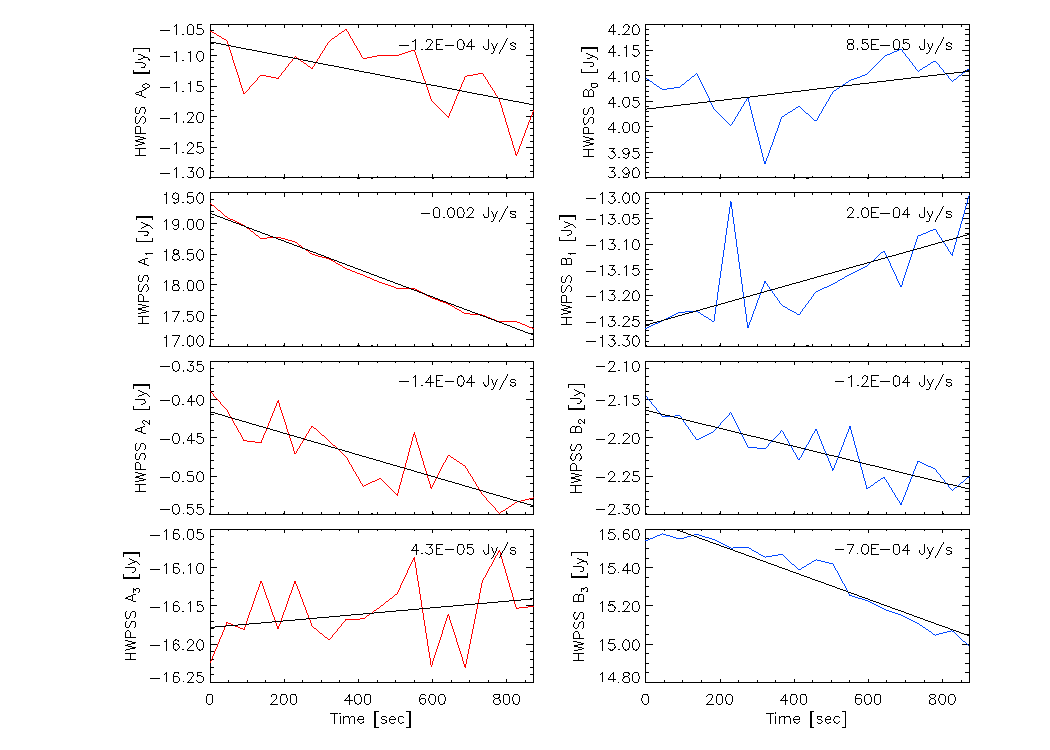
\includegraphics[%
      width=1.\linewidth,keepaspectratio]{figures/template_drift.pdf}
    \caption{Linear fit coefficient and HWP template amplitudes ratio, considered fixed on small chunks of data,
      for a KID and all scans of 3C 286. The amplitudes The four harmonics represented here show
      the percentage variation with the time of HWP template harmonics. The drift in
      time is of the order of 10$^{-3}$ per second. 
      Harmonics of upper order show the same
      trend.{\nico gain space on these figures (Nico)}}
    \label{time_drift}
  \end{center}
\end{figure}

\begin{figure*}
  \begin{center}
%Uncorrected 1 mm
     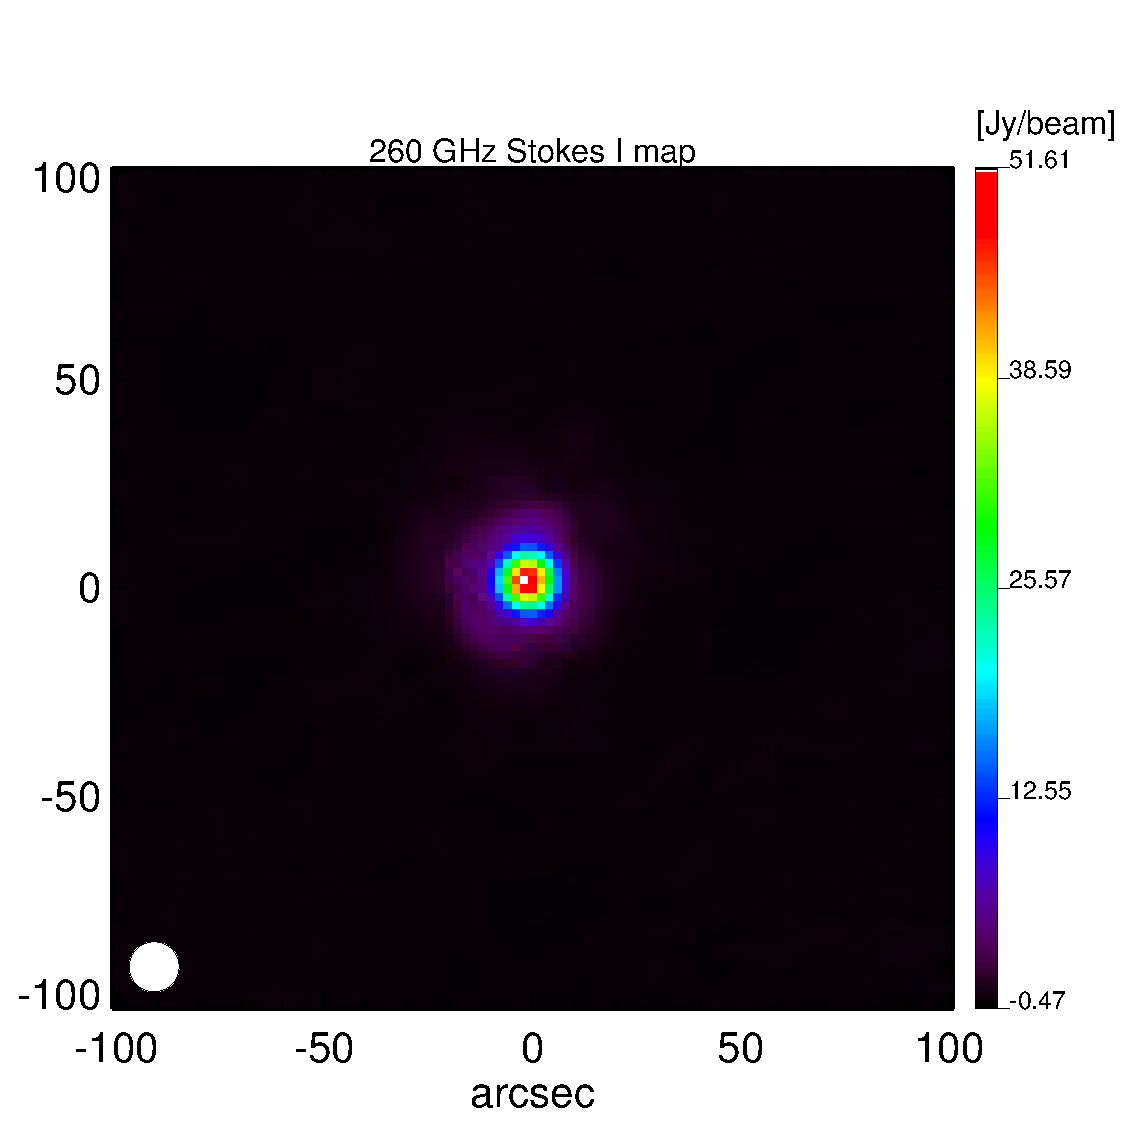
\includegraphics[%
      width=0.30\linewidth,keepaspectratio]{figures/Uranus_I_map.pdf}
   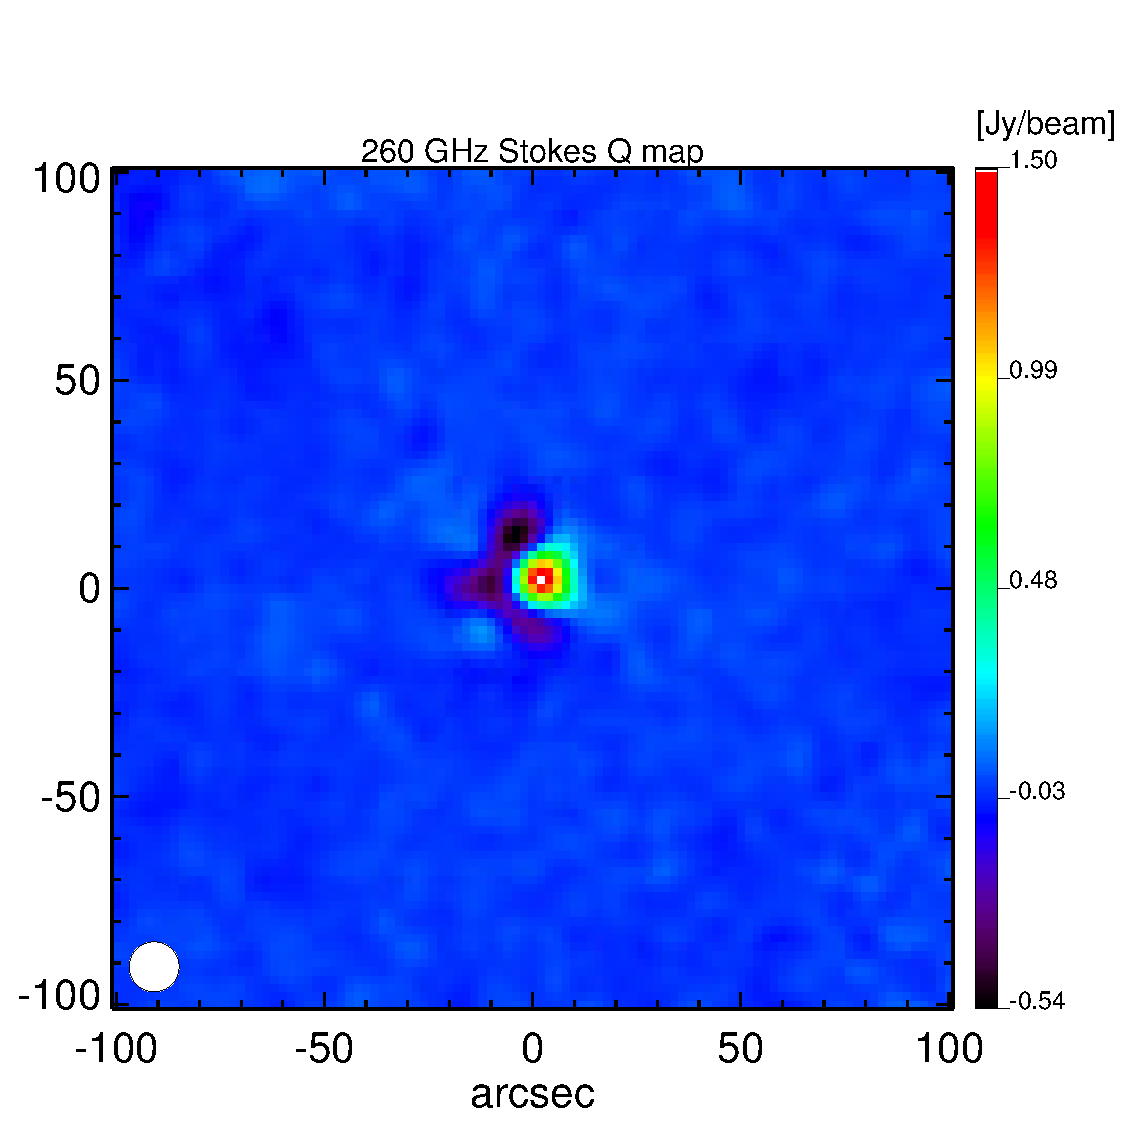
\includegraphics[%
      width=0.30\linewidth,keepaspectratio]{figures/Uranus_Q_map.pdf}
    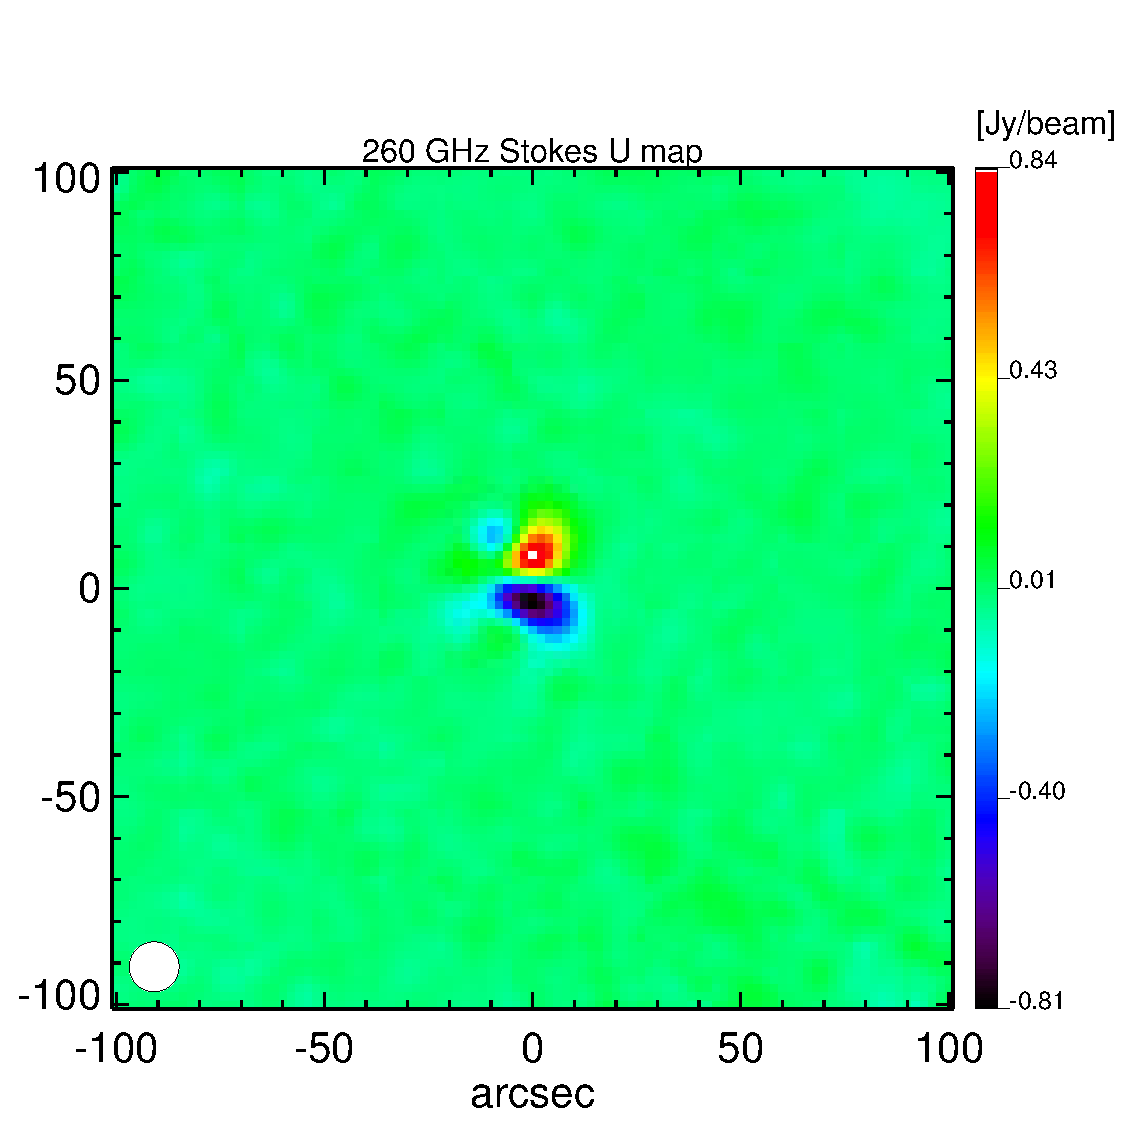
\includegraphics[%
      width=0.30\linewidth,keepaspectratio]{figures/Uranus_U_map.pdf}
 
 %Corrected 1 mm
      
          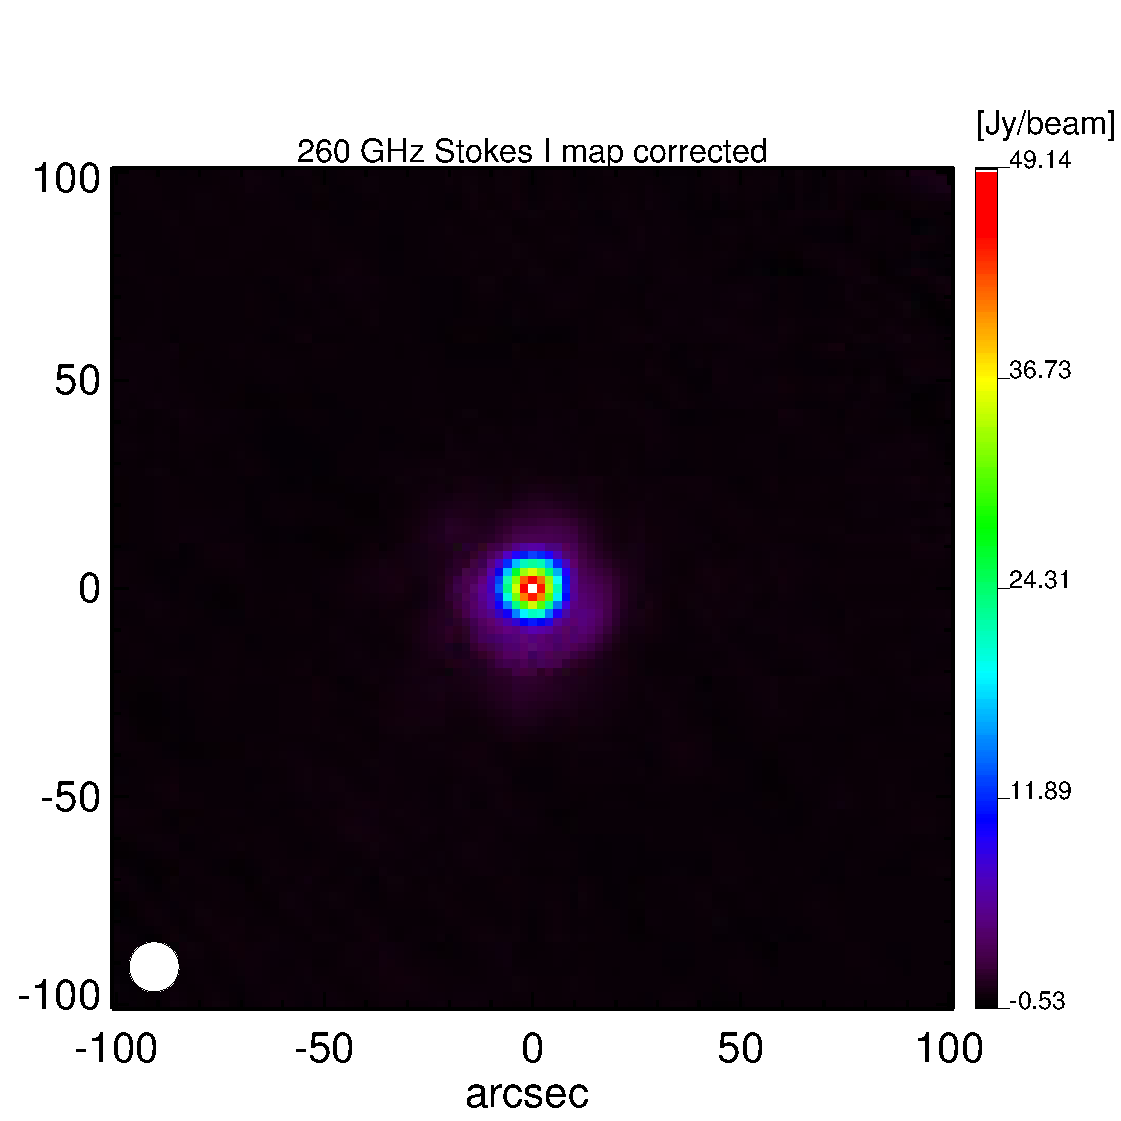
\includegraphics[%
      width=0.30\linewidth,keepaspectratio]{figures/Uranus_I_map_corr.pdf}
    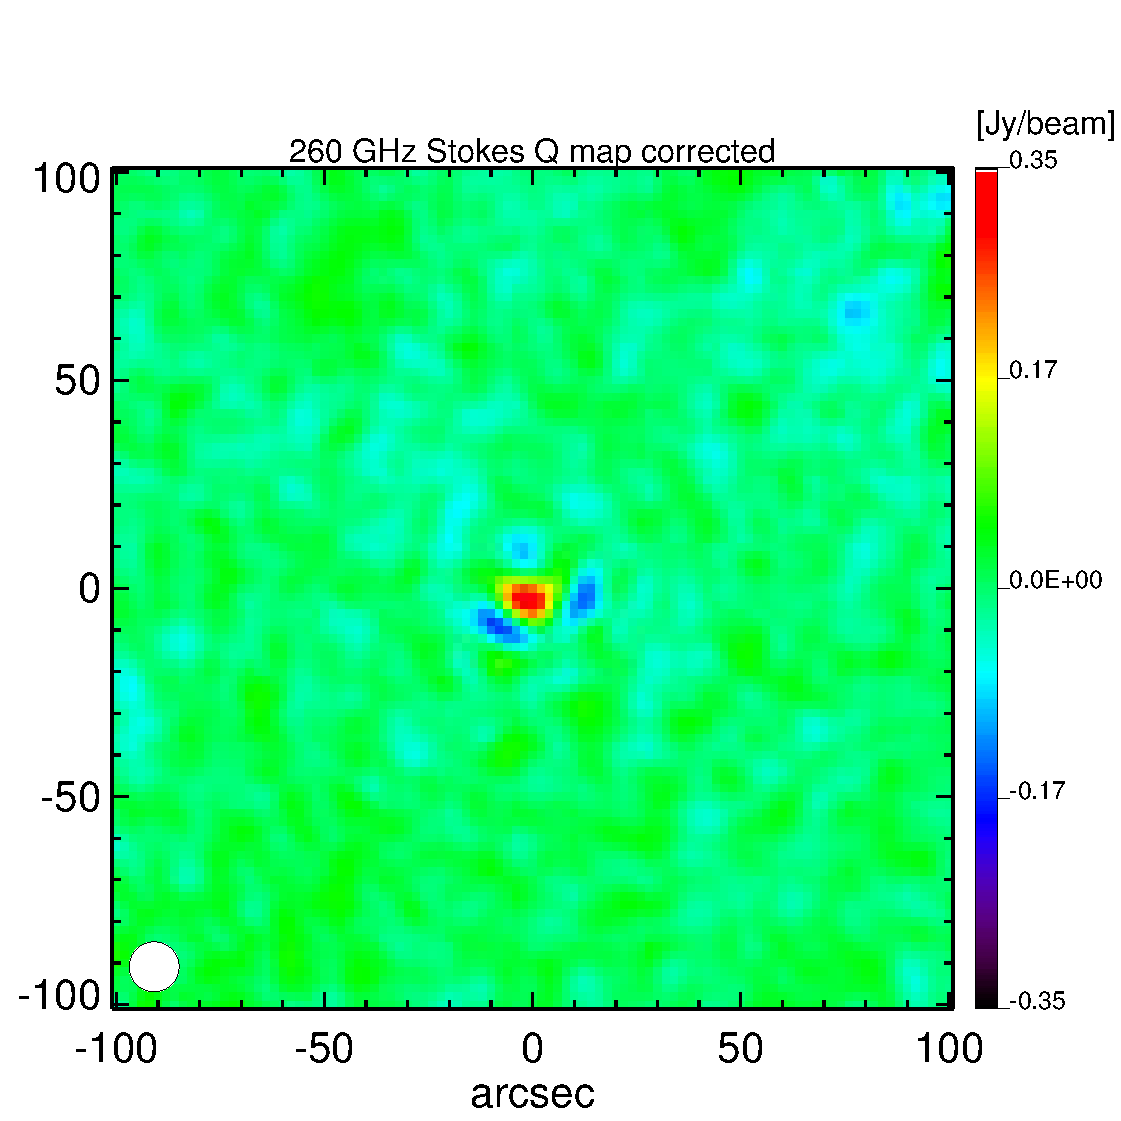
\includegraphics[%
      width=0.30\linewidth,keepaspectratio]{figures/Uranus_Q_map_corr.pdf}
    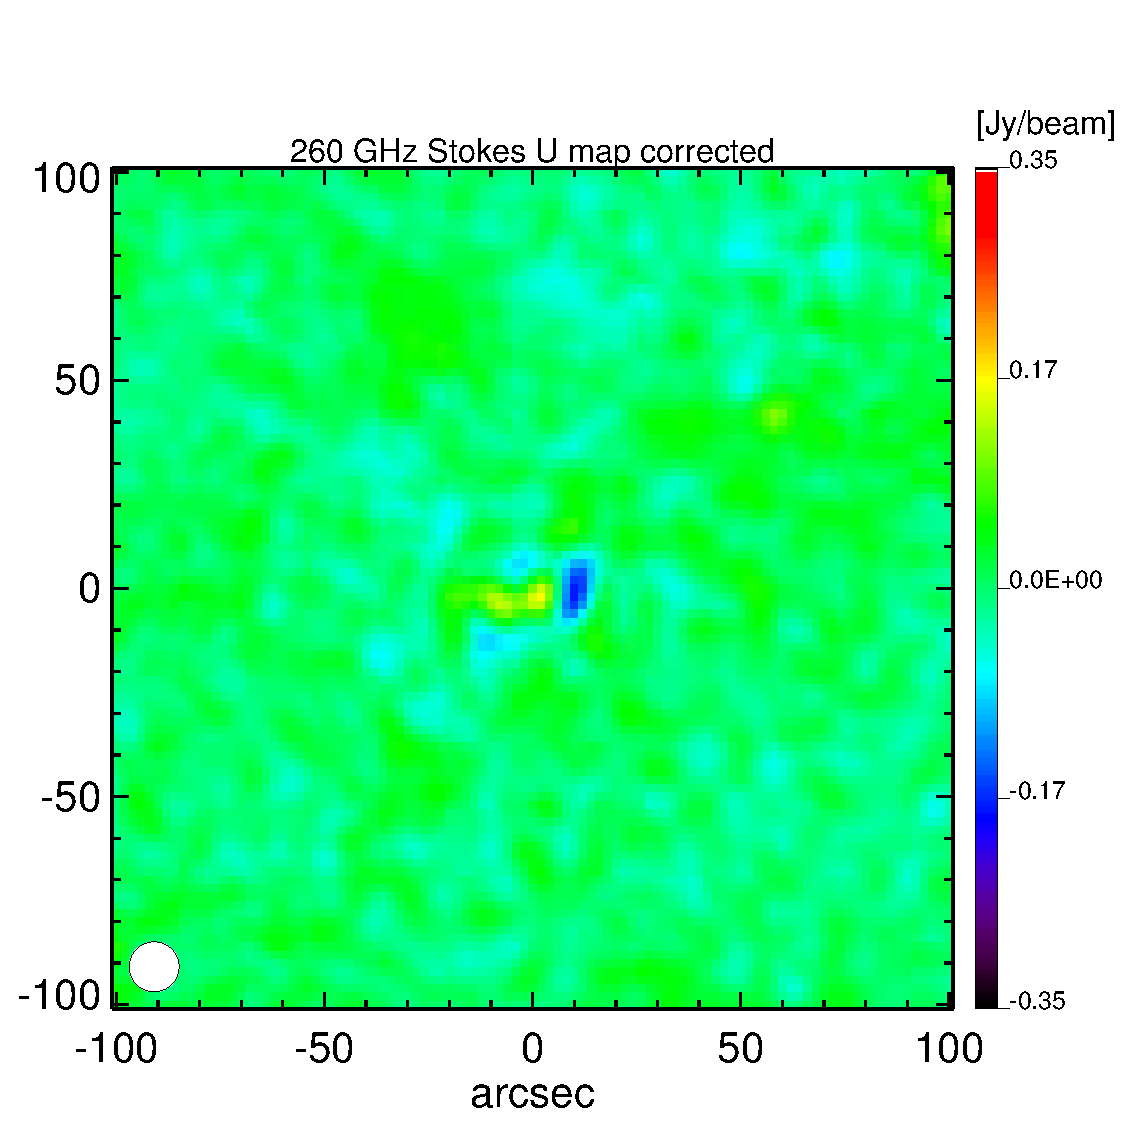
\includegraphics[%
      width=0.30\linewidth,keepaspectratio]{figures/Uranus_U_map_corr.pdf}

%Uncorrected 2 mm

     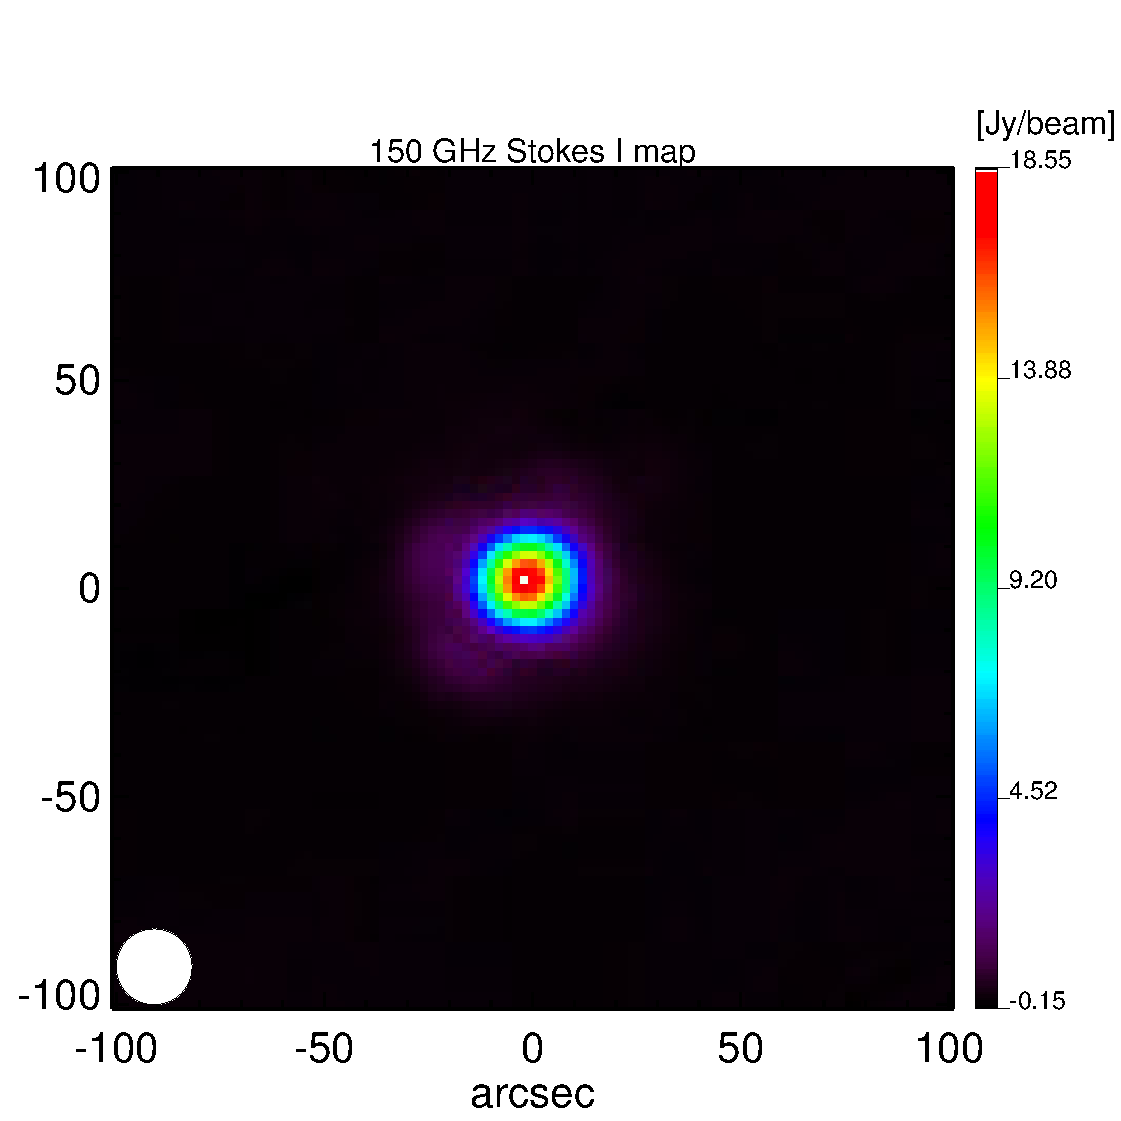
\includegraphics[%
      width=0.30\linewidth,keepaspectratio]{figures/Uranus_I_map_2mm.pdf}
    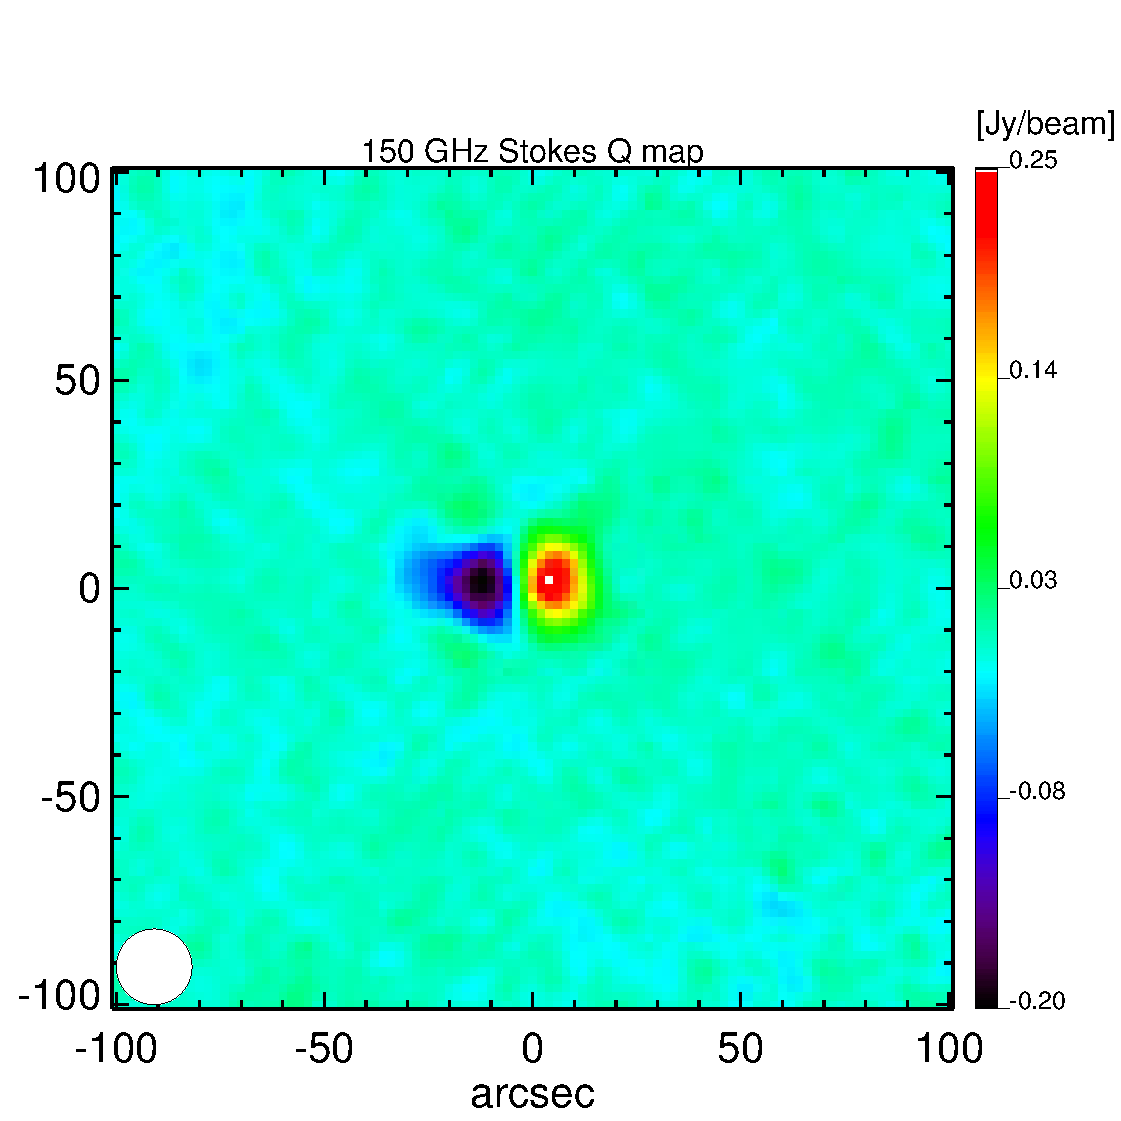
\includegraphics[%
      width=0.30\linewidth,keepaspectratio]{figures/Uranus_Q_map_2mm.pdf}
    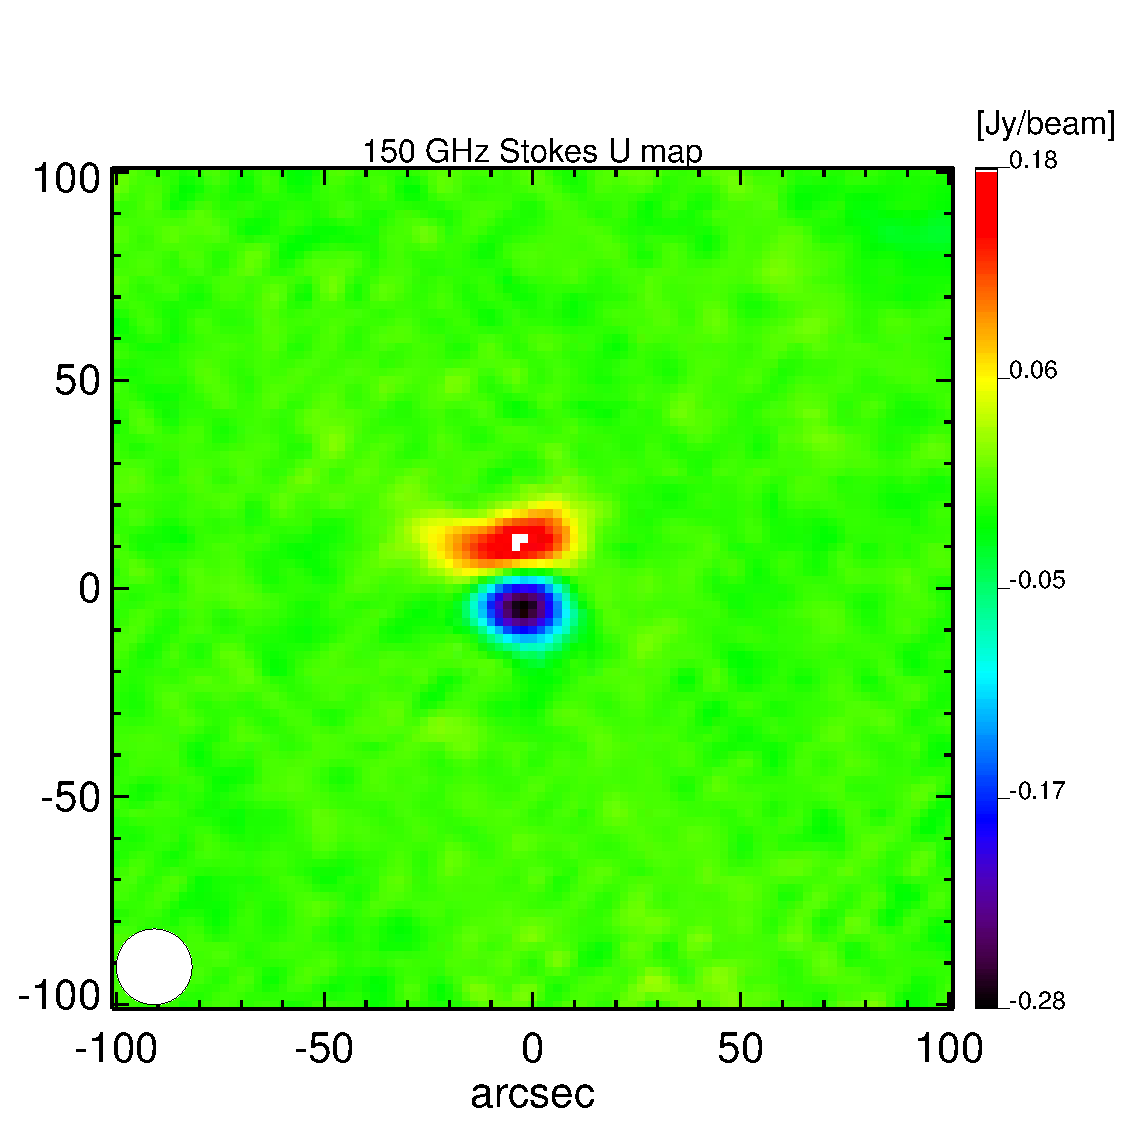
\includegraphics[%
    	width=0.30\linewidth,keepaspectratio]{figures/Uranus_U_map_2mm.pdf}
  %Corrected 2 mm
         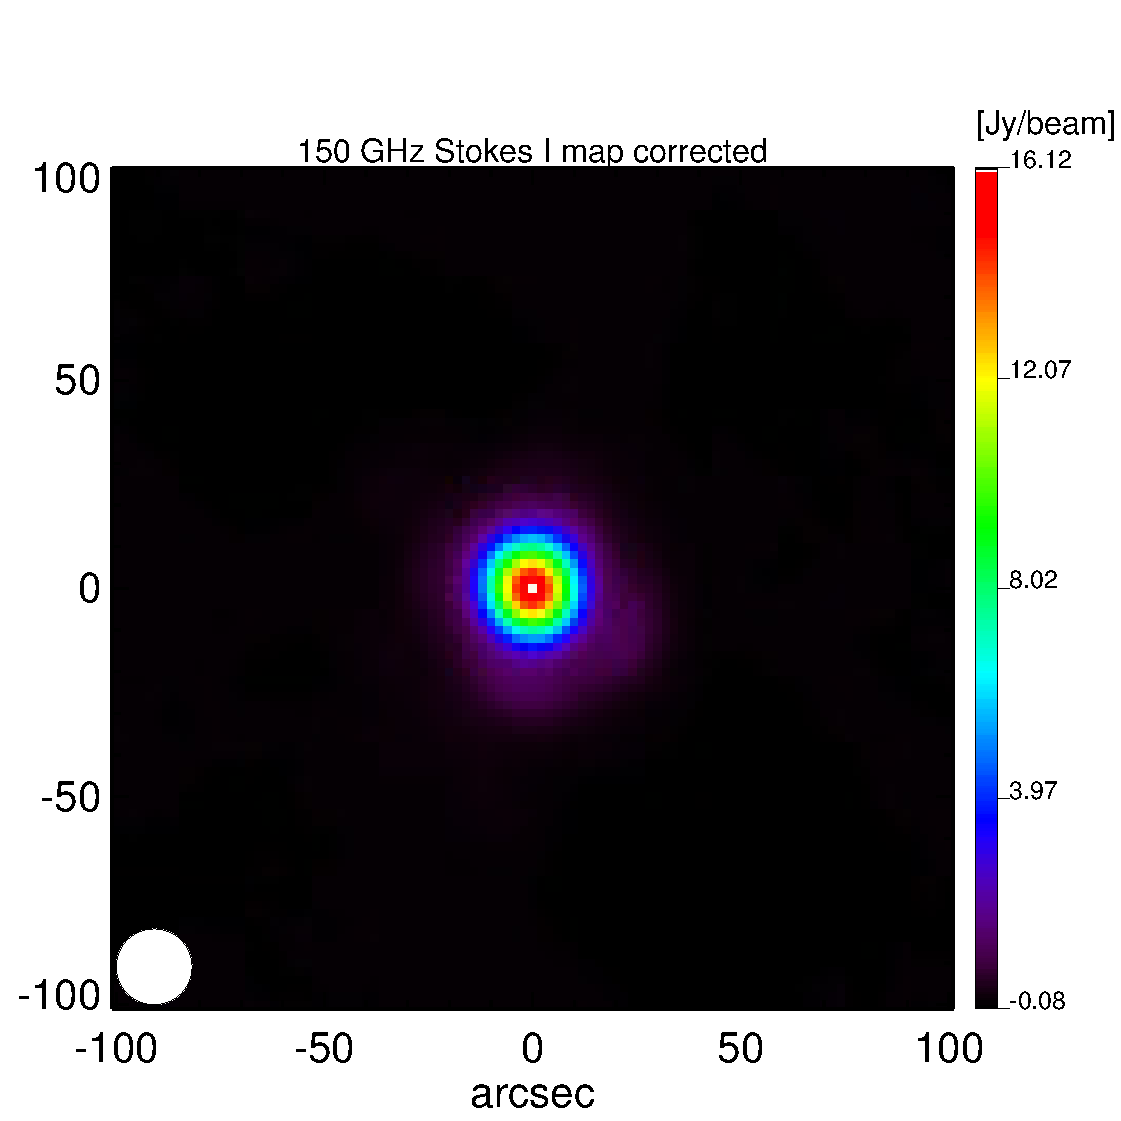
\includegraphics[%
      width=0.30\linewidth,keepaspectratio]{figures/Uranus_I_map_2mm_corr.pdf}
    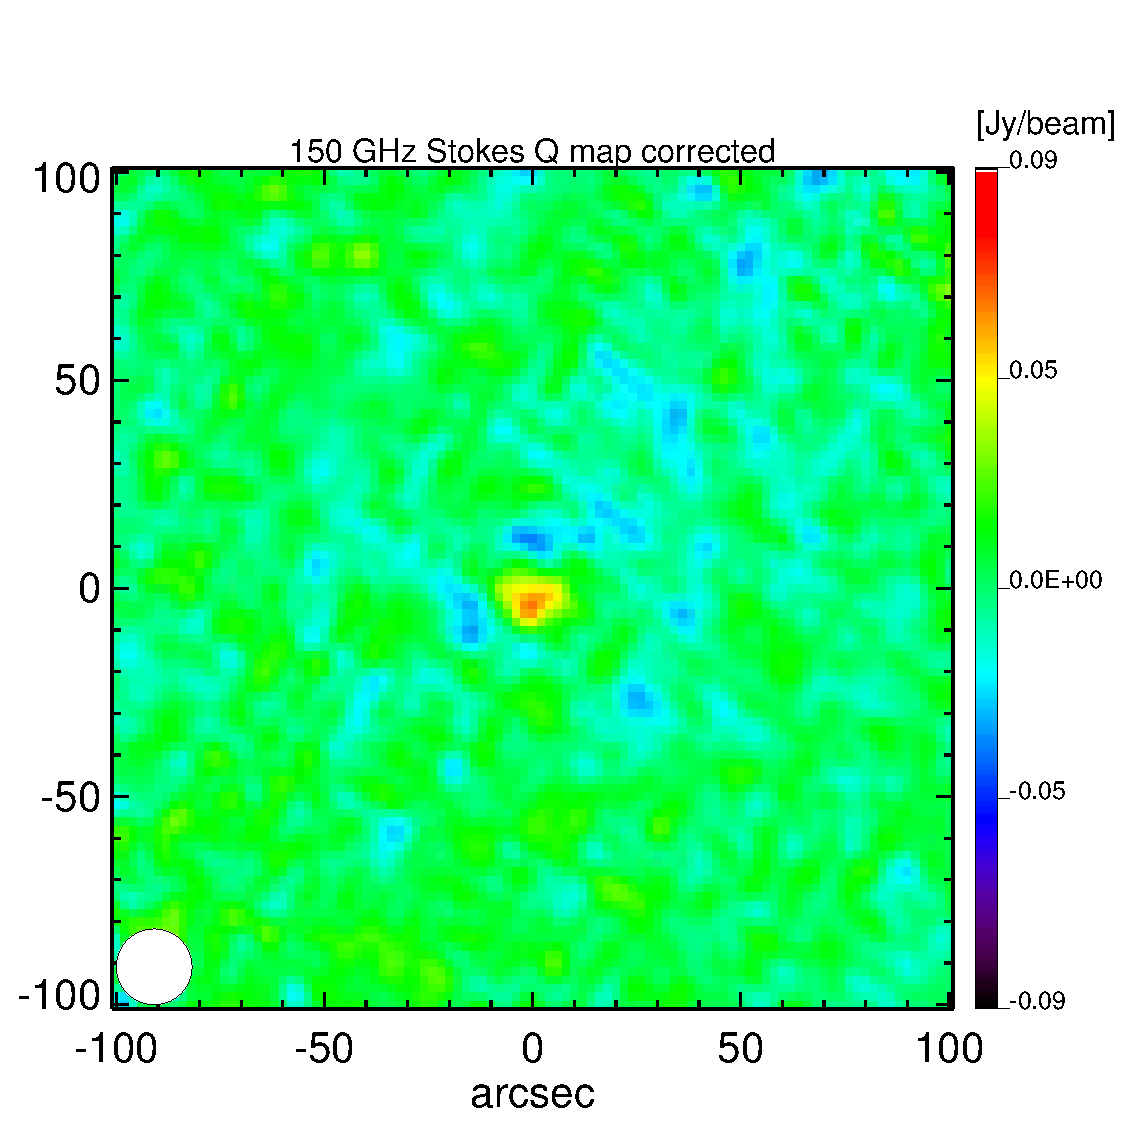
\includegraphics[%
      width=0.30\linewidth,keepaspectratio]{figures/Uranus_Q_map_2mm_corr.pdf}
    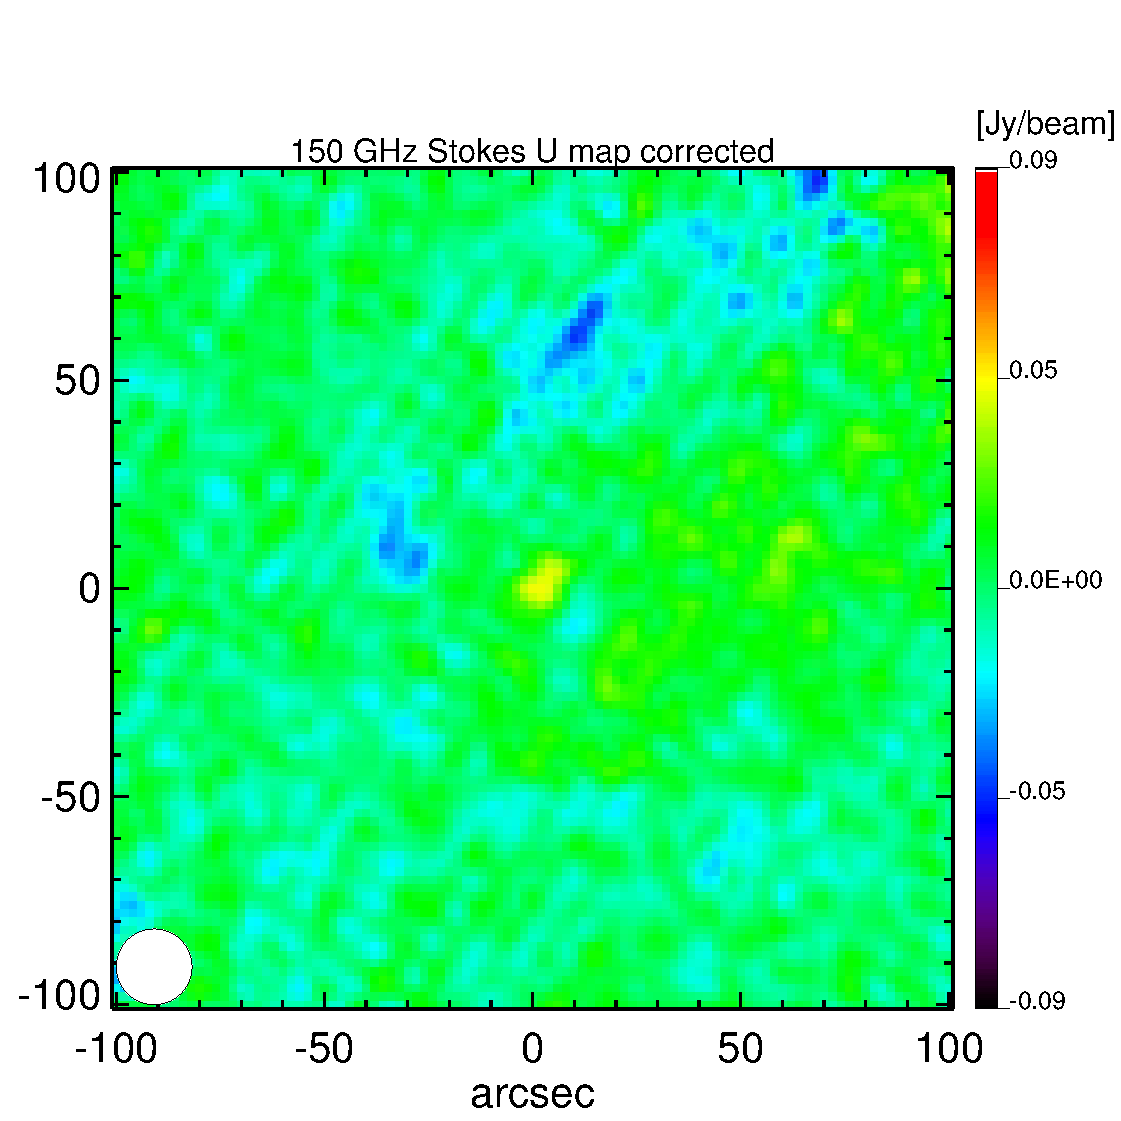
\includegraphics[%
      width=0.30\linewidth,keepaspectratio]{figures/Uranus_U_map_2mm_corr.pdf}
  %Corrected 2 mm
  \caption{ Q and U maps of Uranus (Nasmyth coordinates) showing the systematic
    effect {\nico say Leakage ?} at 260 GHz (top) and 150 GHz (bottom)
    before and after correction. Mind the color scales. }
  \label{fig:uranus_lkg}
  \end{center}
\end{figure*}


\begin{figure*}[h]
  \begin{center}
  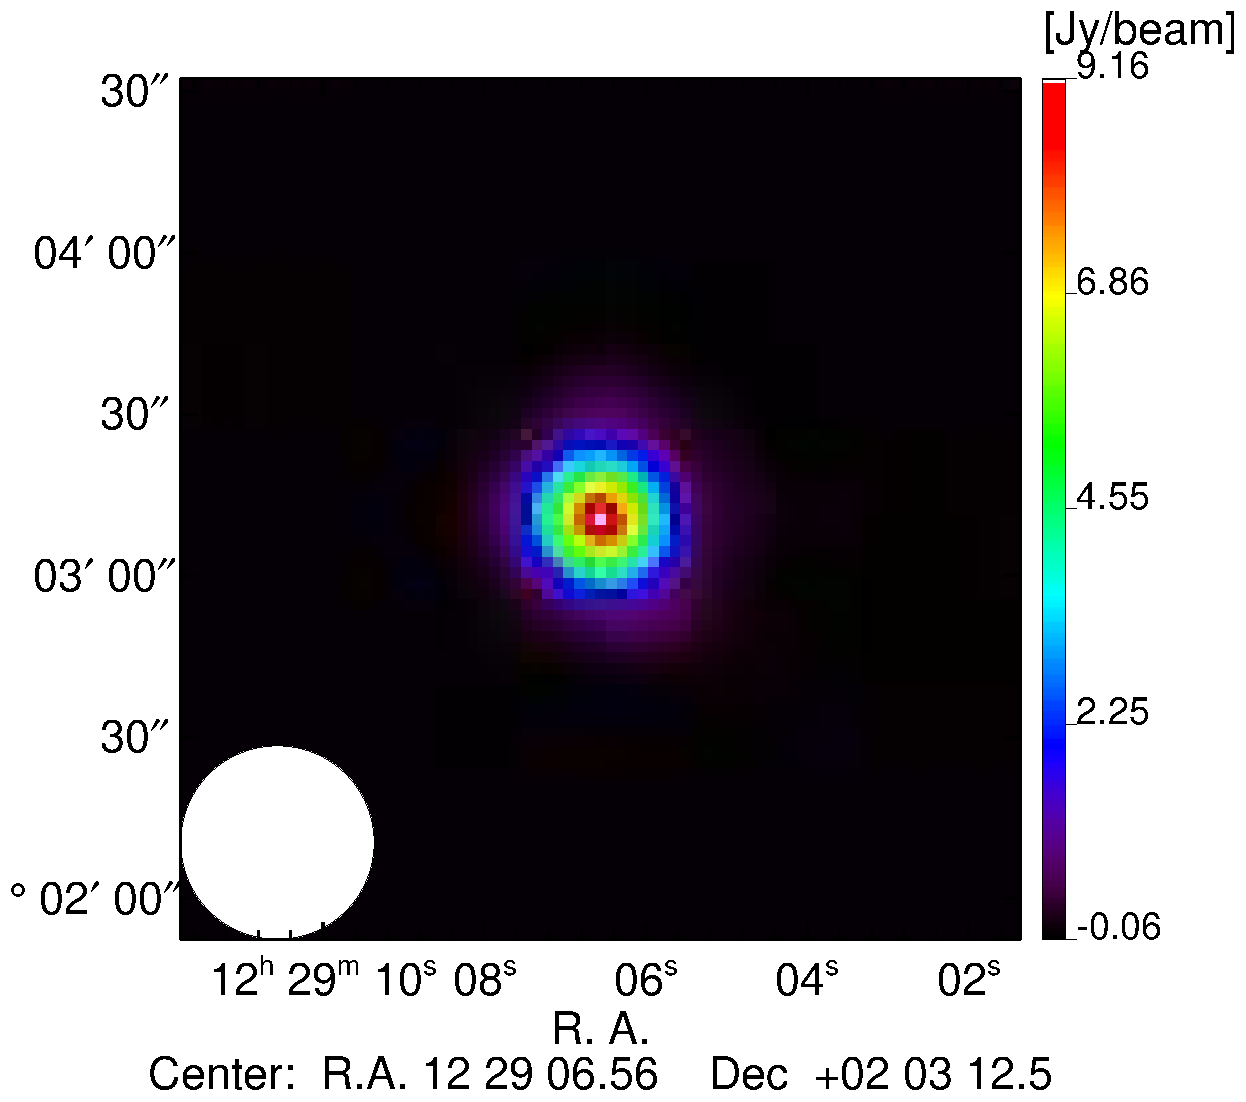
\includegraphics[%
      width=0.33\linewidth,keepaspectratio]{figures/3C273_I_map_2mm.pdf}
    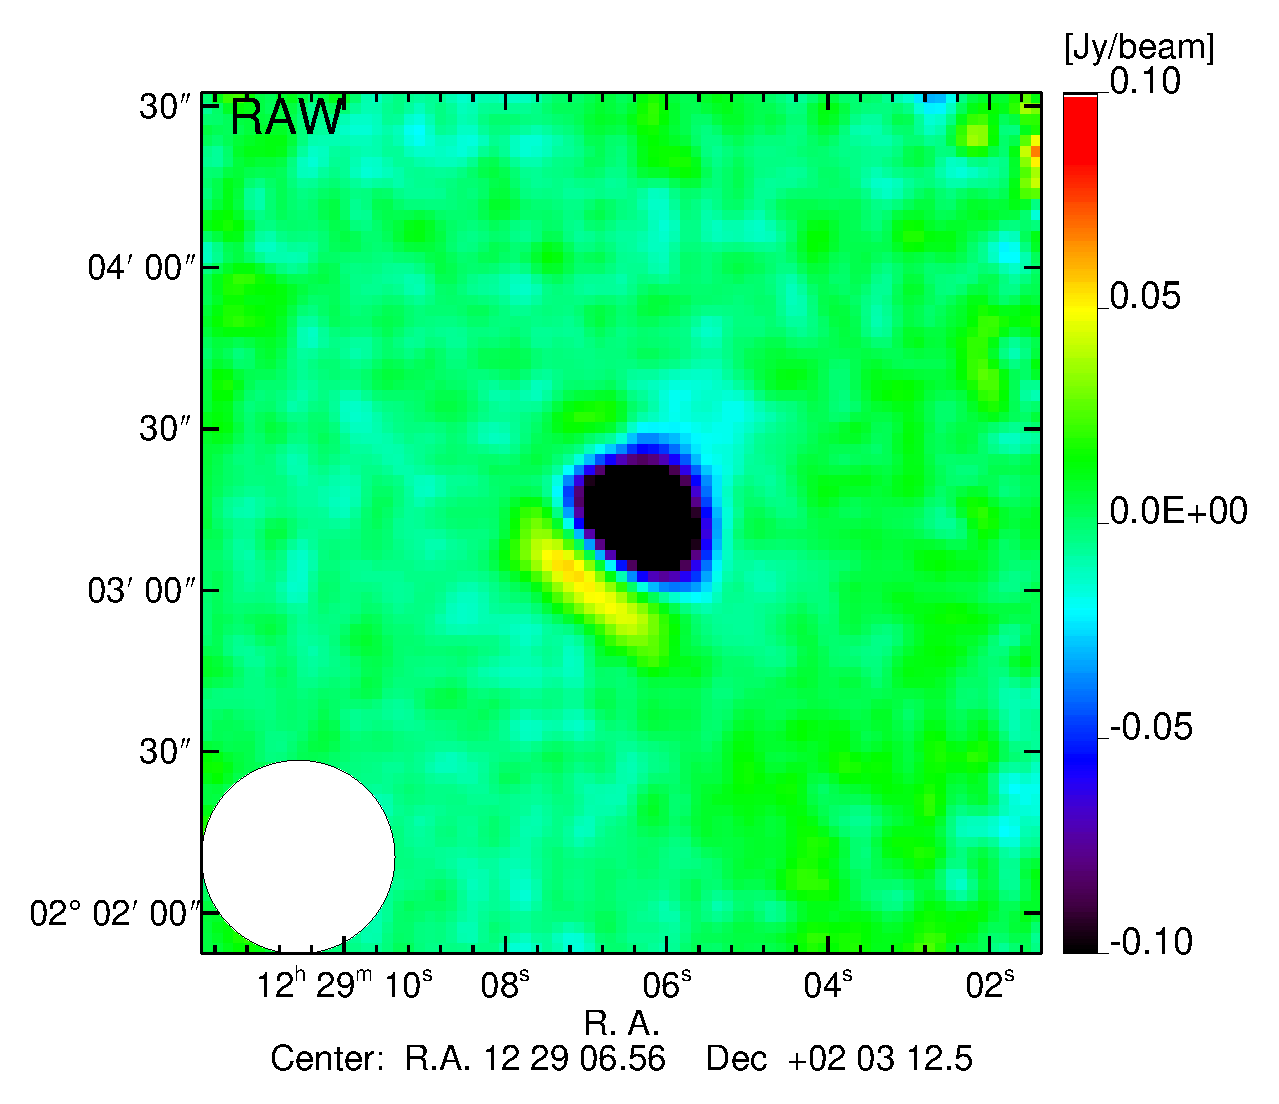
\includegraphics[%
      width=0.33\linewidth,keepaspectratio]{figures/3C273_Q_map_2mm.pdf}
        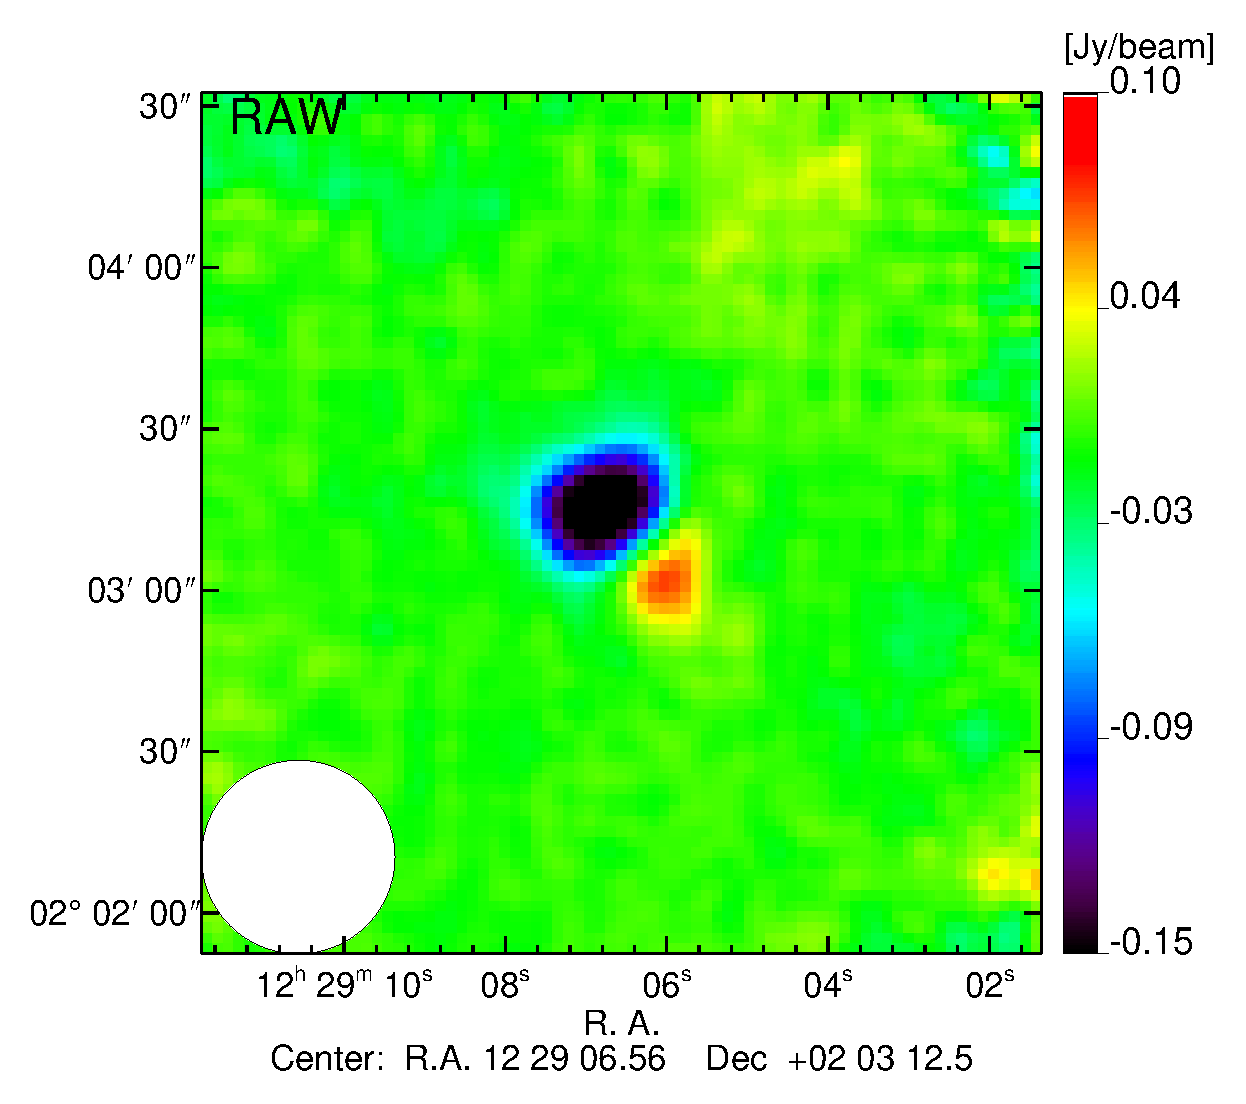
\includegraphics[%
      width=0.33\linewidth,keepaspectratio]{figures/3C273_U_map_2mm.pdf}
       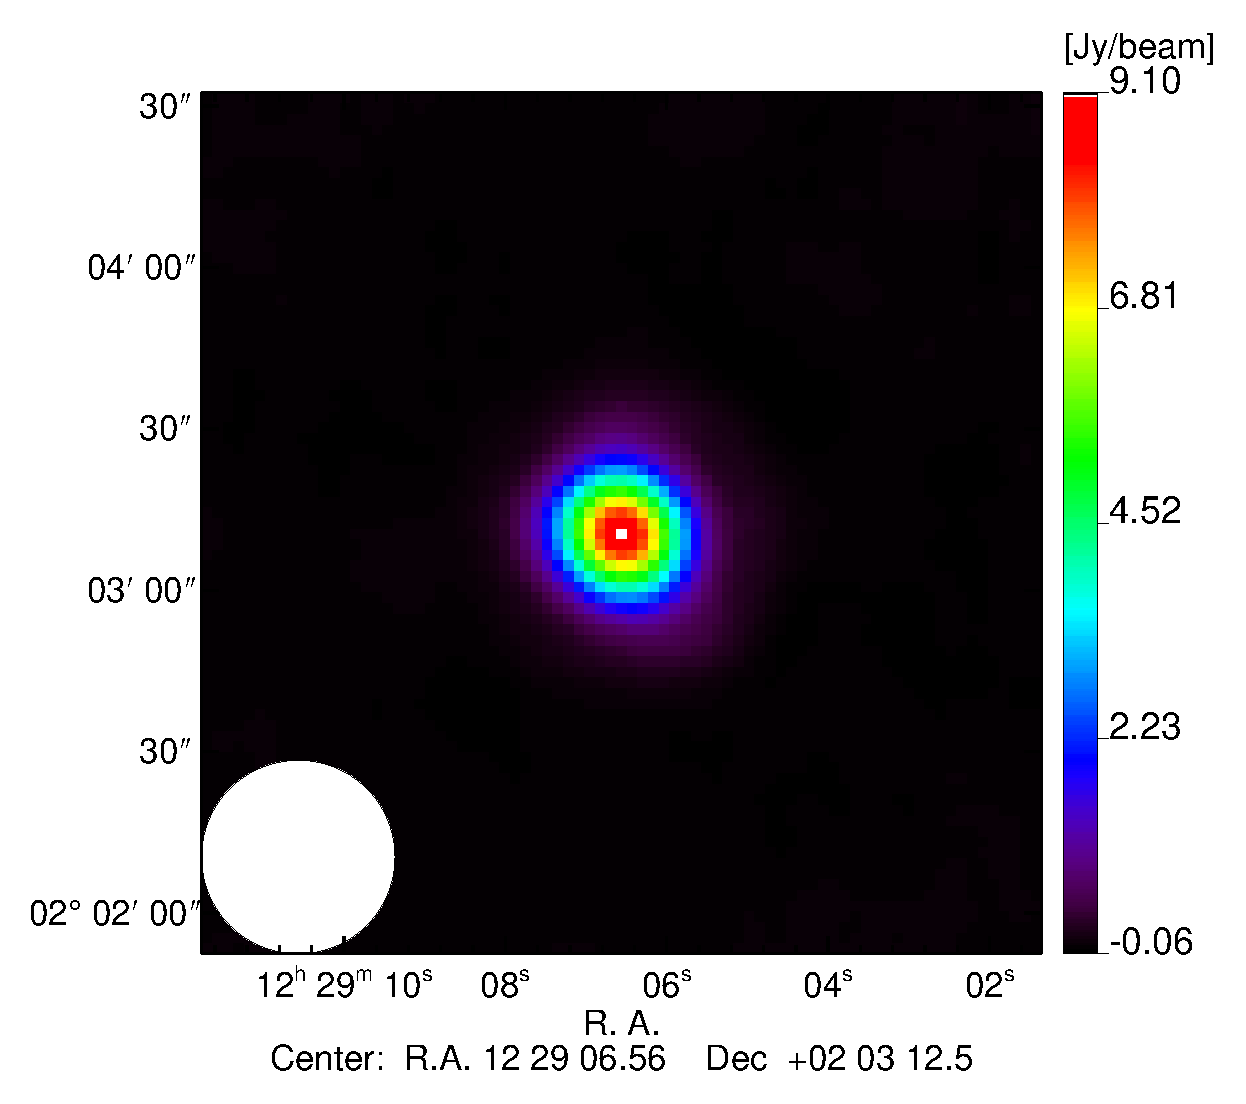
\includegraphics[%
      width=0.33\linewidth,keepaspectratio]{figures/3C273_I_map_2mm_corr.pdf}  
   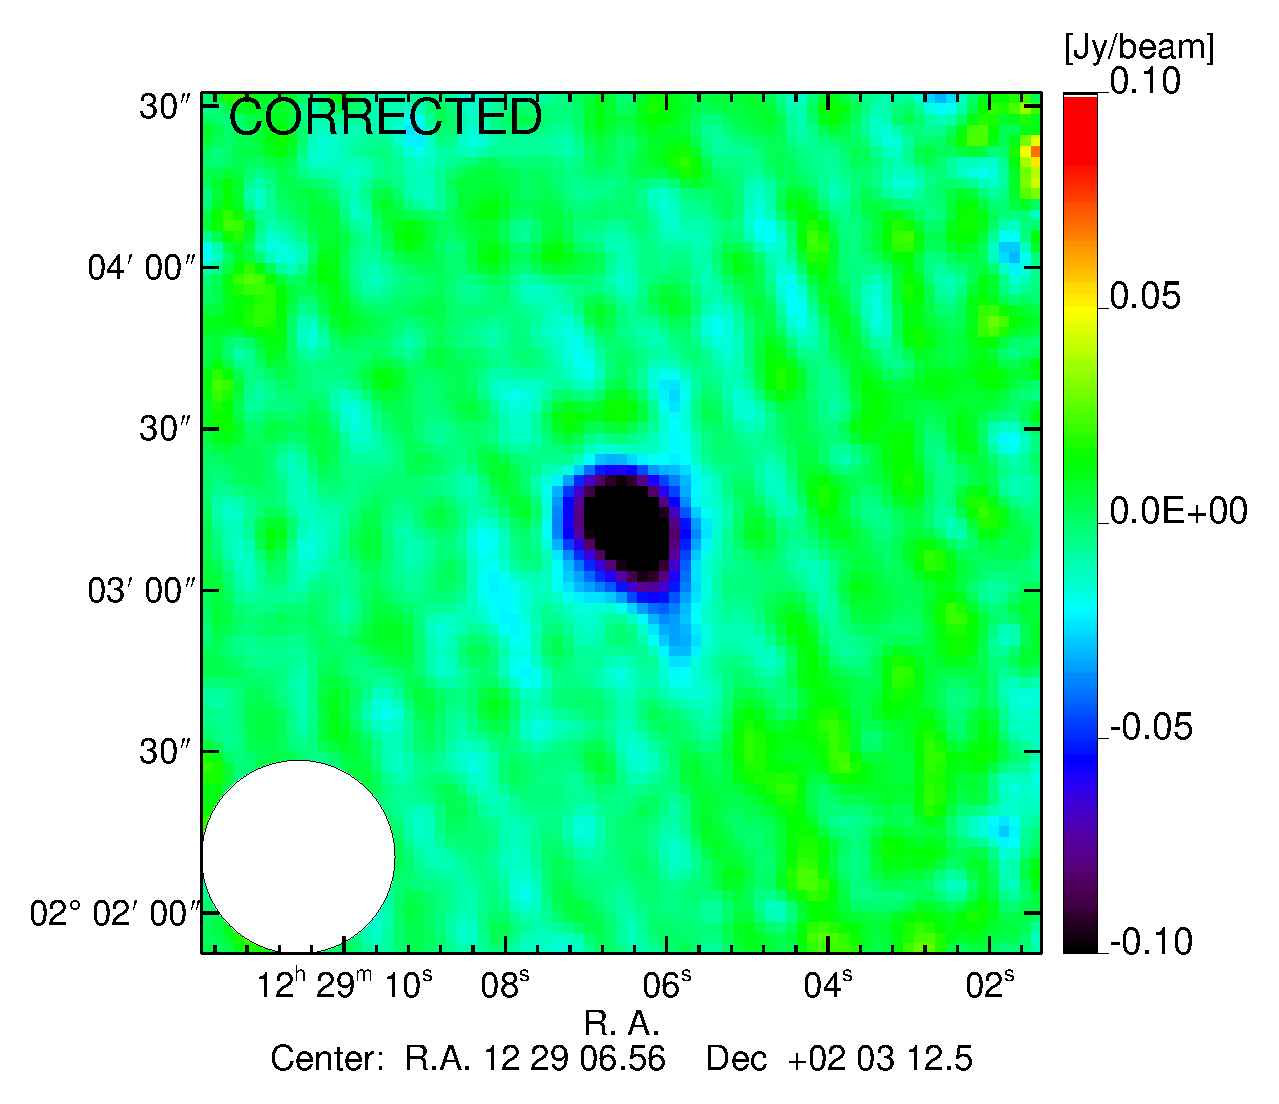
\includegraphics[%
      width=0.33\linewidth,keepaspectratio]{figures/3C273_Q_map_2mm_corr.pdf}
    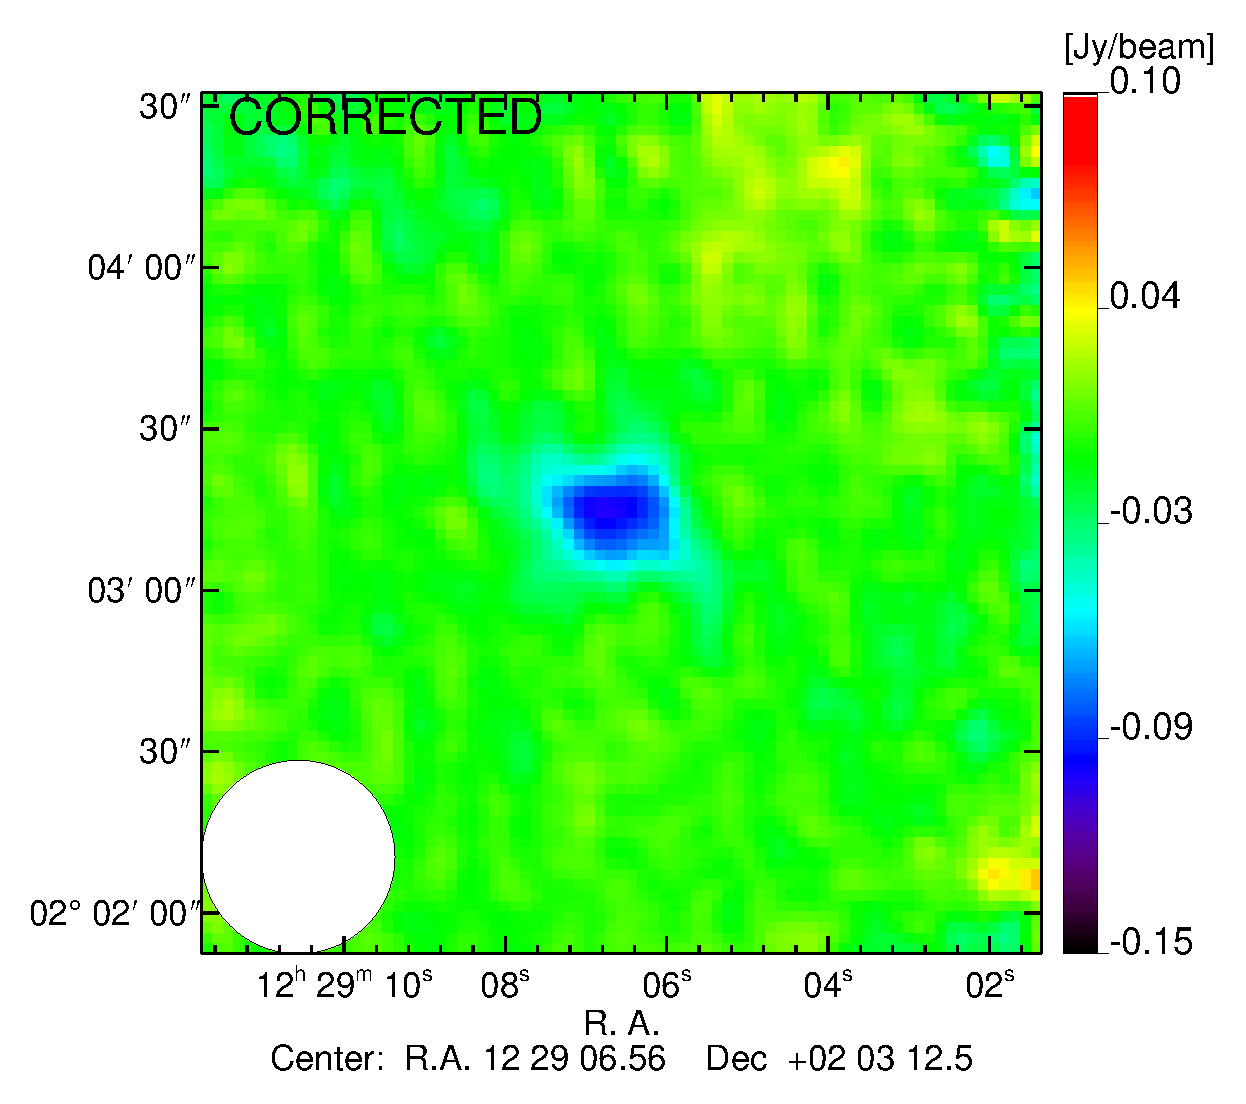
\includegraphics[%
      width=0.33\linewidth,keepaspectratio]{figures/3C273_U_map_2mm_corr.pdf}
      \caption{{\bf Top}: $I$, $Q$, $U$ maps of the quasar 3C 273 observed at 150 GHz
      before correction for the leakage effect. {\bf Bottom}: $I$, $Q$, $U$ maps after correction. The polarisation angle and degree are reported in the table \ref{tab:table_quasar}.}
    \label{3c273_ex}
  \end{center}
\end{figure*}

  
Imperfections of the HWP modulate the background and lead to a strong
additionnal signal on the timelines, highly peaked at harmonics of the HWP
rotation frequency $\nu_P$ as shown on Fig.~\ref{spectre_iqu}. Such a HWP
Synchronous Signal (HWPSS) has already been observed by Maxima
\citep{johnson2007} and EBEX \citep{ebex} {\nico check with polarbear and
  other experiments quoted in introduction}. Like them, we observe that the signal
is well fitted by a sum of harmonics of $\nu_P$, with amplitudes slowly and
linearly drifting with time at the level of {\nico below ?!} 10$^{-3}$ per second.
(Fig.~\ref{time_drift}). We therefore explicitly model this additional signal
as
{\nico
\begin{eqnarray}
HWPSS(t) &= \sum_{n=1}^{8}& (A_n+ \epsilon_{A_n}t)\cos n\omega_Pt\nonumber\\
&& +(B_n+\epsilon_{B_n}t)\sin n\omega_Pt.
\label{eq:hwpss}
\end{eqnarray}
}
We collect all samples of a kid into a vector ${\bf v}$, build a matrix $T$
whose columns are {\nico $\cos n\omega_Pt$, $t\cos n\omega_Pt$, $\sin n\omega_Pt$
and $t\sin n\omega_Pt$}. We then perform a maximum likelihood fit giving the
same weight to all samples ${\bf a} =
(T^TT)^{-1}T^T{\bf v}$ to derive ${\bf a}$, a vector containing amplitudes $A_n$,
$B_n$ and $\epsilon_{A_n}$ and $\epsilon_{B_n}$. With this amplitudes in hand,
we can build a model of the HWPSS in the kid timeline and subtract it.

We could in principle improve this fit by using only samples far from the source
when possible. However, the HWPSS is about {\color{red}XXX~Jy} peak to peak,
therefore much stronger than the astronomical signals we observe, and not sky
synchronous. We thus found that it did not make any difference to take this
extra precaution, and as far as this technical run is concerned, we did not
apply this masking. {\color{red} we need to conclude this section by a plot
  showing how well this model subtracts the ``true'' HWPSS. We must also repeat
  that we actually care only about effects around $4\nu_P$}\\

We can then summarize our map making algorithm as follows. Let's denote by
$\delta$ the elevation of the considered kid and $\eta$ the parallactic angle:

\begin{enumerate}
\item Fit and subtract the HWPSS from each kid
\item Make two extra copies of the obtained TOI's. Multiply one of them by
  $\cos[4\omega_Pt + 2(\delta-\eta)]$ and lowpass at 2.9~Hz to obtain a $Q$-timeline. Multiply the other
  one by $\sin[4\omega_Pt+2(\delta-\eta)]$, lowpass at 2.9~Hz to obtain a
  $U$-timeline. Simply lowpass the original one at 2.9~Hz to have the
  $I$-timeline.
\item Coadd with inverse noise weighting these timelines onto three separate
  maps of $I$, $Q$ and $U$.
\end{enumerate}

\subsection{Optics related systematic effects}




%% {\color{green} to be rephrased and placed somewhere else: As we have discussed
%%   above the power spectrum of the TOIP is consisting with a flat spectrum. The
%%   negative and positive beam observed in the leakage maps compensate each other
%%   and smooth the effect.  Taking a convolution between the atmospherical spread
%%   signal, the Stokes intensity $I$ map with the characteristic 1/f component of
%%   noise, and the leakage beam in $Q$ and $U$ we found that the two component
%%   compensation drowning the effect in a white noise.}

In order to estimate the level of the instrumental polarization at the telescope
we repeatedly observed Uranus, that is unpolarized, bright (47.2~Jy at 1mm,
16.4~Jy at 2mm) and small ({\color{Red}XXX arcsec diameter}) compared to our
beams. Not only do we find non zero polarization, but the shapes of $Q_{Uranus}$
and $U_{uranus}$ also differ from that of total power beam
(Fig.~\ref{fig:uranus_lkg}). Indeed, we observe a mainly dipolar pattern,
partially consistent between the two bands, with a peak to peak amplitude at the
level of 3\% of the total intensity peak. Such an effect has already been
observed on previous experiments, e.~g.~BICEP ({\color{red}ref TBC}), QUaD
({\color{red}ref TBC}), PILOT ({\color{red}ref TBC, etc...}). Monitoring of this
effect at different elevation angle shows that it is fixed in Nasmyth
(i.e.~cabin) coordinates. Note that this effect does not lead to a direct
scaling of the sky noise into polarization at the 3\% level because in this
case of diffuse emission, the integral of the term and not only the peak value
must be considered. At best, it therefore creates a contamination at the
{\color{red} XXX exact level TBC and complement this sentence with a remark on
  the possibility to decorrelate Q and U timelines like I.}

So far, we still lack a convincing physical interpretation. However, formally,
it can be considered as leakage from total power $I$ into $Q$ and $U$. To
mitigate this effect, we have developped the following algorithm. We denote
quantities unaffected by any beam with a $_0$ index, and with a $^N$
superscript, quantities evaluated in Nasmyth coordinates. Like in
Sect.~\ref{se:pol_module}, $\psi$ {\nico check consistency} is the
polarization observation angle that accounts for both the HWP angle and the
parallactic angle. Leaving noise aside for the sake of readability, we model the
noiseless measurement of a kid $k$ at time $t$ such as the sum of the signal
convolved by the instrumental main beam $B_I$ and of an extra leakage term from
the signal intensity into $Q$ and $U$:

\begin{eqnarray}
S_k &=& B_I * (I^N_0 + Q^N_0\cos2\psi + U^N_0\sin2\psi) \nonumber \\
       &&+ L_{IQ}*I^N_0\cos2\psi + L_{IU}*I^N_0\sin2\psi,
\label{eq_leak}
\end{eqnarray}

where $*$ denotes convolution. As Uranus can be considered as a point source
with respect to the \nika's angular resolution, the $Q^N$ and $U^N$ maps give
directly the $L_{ IQ}$ and $L_{ IU}$ beams, up to an absolute calibration factor
that is straightforward to scale {\nico say a word on this scale, how
  sensitive are we to its choice} by comparing to the $I$ map. All that is needed
now to subtract the leakage terms from the measurements is an estimate of
$I^N_0$. While we cannot deconvolve the observed $I$ map from the instrumental
beam $B_I$ with perfect accuracy, this is actually not needed since $I^N_0$ must
be convolved back by $L_{IQ}$ and $L_{IU}$. This sets a scale in Fourier space
up to which division by the instrumental beam $B_I$ remains accurate enough
compared to knowledge on $B_I$ and on map noise, and above which multiplication
by the leakage beams ensures a regularizing damping. We thus summarize our
correction process as:

\begin{enumerate}
\item With the demodulation and projection techniques presented in
  Sect.~\ref{data_analysis}, build maps of $I$, $Q$ and $U$ of the observed
  signal in equatorial coordinates. This map can be the result of multiple scans to have
  the best possible signal to noise.
% This map can be the combination of multiple scans to
%  have the best signal to noise S/N.
\item Rotate this map in Nasmyth coordinates to obtain $I_N$, $Q_N$ and $U_N$
  for the current scan.
\item Build the convolution/deconvolution kernels $L_{IQ}/B_I$ and $L_{IU}/B_I$
  in Fourier space from observations of Uranus.
\item Multiply the Fourier transform of $I^N$ by these kernels in Fourier space
  and transform the result back into real space to have maps of leakages from
  $I$ into $Q$ and $U$.
\item Deproject the obtained maps with the actual scan pattern to produce
  timelines that are then subtracted from the data TOIs.
\item Project these corrected TOIs onto final maps.
\end{enumerate}

The rotation from equatorial to Nasmyth coordinates introduces a small
error. Indeed, the rotation angle combines the elevation and the parallactic
angles that are not constant during the scan. Ideally, we should rotate the
equatorial map continuously in time. Although doable in principle, at the
expense of computation speed, this is only an uncertainty on the error and is thus
of second order {\nico give a rough estimate of the effect to justify this
  a bit better. Doesn't step one actually improve the quality of the estimate
  when we stack scans taken at different angles the leakage should actually
  average down in radec, therefore leading to purer map even before correction }


%% The deconvolution/convolution steps 3 and 4 are performed at the same time in Fourier
%% space:
%% 
%% \begin{equation}
%% (I^N_0*L_{IQ})(k) = I^N_0(k) \times L_{IQ}(k) \simeq I^N(k)/B_I(k)\times L_{IQ}(k)
%% \end{equation}

%% The ratio $L_{IQ}(k)/B_I(k)$ is tapered so that the division by decreasing terms
%% of $B_I(k)$ when $k$ increases is counterbalanced by the deaming of
%% $L_{IQ}(k)$.
Fig.~\ref{uranus} shows $I$, $Q$, $U$ maps of Uranus (expected to be
unpolarised) exhibiting the systematic effect (top panel) observed in $Q$ and
$U$ maps as discussed above.  The algorithm of correction is then applied to
another scan to check the residual instrumental polarisation.  The
algorithm used has dropped from 3\% of the total intensity to below 1\%.  In
order to give an example on a polarised source we show the maps obtained for the
quasar 3C273 in Fig.~\ref{3c273_ex}. In this figure we show the maps before
applying the algorithm of correction (left column) and after (right column); the
efficiency of this correction allows us to estimate a more correct polarisation
degree and angle. Here the quasar is taken as example but a proper discussion on
the results obtained in terms of polarisation degree and angle is given in the
calibration section.

% polarization maps the
%% instrumental residual polarisation is estimated to be below 0.1 $\%$ as shown in
%% Fig. \ref{Uranus_corrected}. $I, Q, U$ maps are shown in order to compare
%% directly with the maps uncorrected represented in Fig. \ref{uranus}.

\subsection{Calibration}
\label{se:calib}
{\color{green} quasars: know and stable, variable but observed at the same time. End up by
mentioning the remaining discrepencies and likely explanations and why we remain
confident, in particular with the addtional observations of the Crab and OMC1}

In this section, we describe how we calibrate \nika~in polarization mode.

The absolute calibration follows the exact same method as in total power and is
described extensively in \cite{catalano2014} {\color{red} check ref}. Uranus is
our main absolute flux calibrator. We correct for sky opacity using {\it
  skydips}, i.e.~pure elevation scans that help us monitor the response of the
LEKIDs to air mass and hence correct for it. For this polarized technical run,
we have 15\% uncertainty on absolute calibration at 1.25~mm and 10\% at
2.05~mm. Our measured FWHM's are 13.5~arcsec at 1.25~mm and 18.4~arcsec at 2.05~mm.

The calibration of \nika's orientation on the other hand, is specific to this
work. During that period of February 2015, we could observer...


%%==========================================================================================



%% In real conditions there is an additional parasitic signal at harmonics of 1{$\omega$}, 2{$\omega$}, 3{$\omega$} etc, due to imperfections of the HWP. Furthermore, the atmospheric and electronic noise need to be taken into account. 
%% Thus Eq. (\ref{signal_polar}) reads:
%% \begin{eqnarray}
%%  m_{k} &=& \frac{1}{2}\{I + {\rho}_{ pol}[Q\cos(4{\omega}t + 2{\alpha}_{\rm Sky}(p_{\rm t})) + Usin({4{\omega}t} \nonumber \\
%%  	  &+& 2{\alpha}_{Sky}(p_{\rm t})]+ S_{\rm parasitic} ({\omega}t, 2{\omega}t, 3{\omega}t, ...)\} \nonumber \\
%% 	  &+& {\rm atmosphere} + {\rm noise}_{\rm detector}
%%  \label{pol_eq}
%%  \end{eqnarray}
%%  where $p_{\rm t}$ represents the pixel observed at time $t$ and ${\alpha}_{\rm Sky}$ the angle between the telescope reference frame and the local meridian on the sky. 
%% The angle ${\alpha}_{\rm Sky}$ is measured from north to east in the equatorial system as  ${\alpha}_{\rm Sky} = {\tau} - {\epsilon} - {\eta}$,
%% where ${\epsilon}$ represents the elevation, ${\eta}$ the parallactic angle, and ${\tau}$ = 45.54$^{\circ}$ is the tilt of the switch mirror of the Nasmyth system along the elevation axis, which creates an angular offset of the image of the sky on the detectors arrays. 	
%% 



%%  \section{Data analysis}\label{sec:pipeline}
%% In order to calibrate, filter, and project data onto sky maps we developed a
%% dedicated reduction pipeline based on the intensity one described in
%% \citep{catalano2014, adam2014}. The main steps of the processing consist of:
%% \begin{itemize}
%% \item read data time ordered information (TOI): data ordered per kid and regularly sampled with time.
%% \item TOI calibration: the absolute calibration is applied to these TOIs and an
%%   atmospheric absorption correction performed. The planet Uranus is the primary
%%   calibrator for the {\it NIKA} absolute calibration. The calibration factor is
%%   derived by fitting a Gaussian of fixed angular size on the reconstructed maps
%%   of Uranus \citep{catalano2014}. The sky maps are corrected for the atmospheric
%%   contribution rescaling the observed signal by what that would be obtained in
%%   the absence of the atmosphere. This is achieved via the elevation scan
%%   technique (\emph{skydip}).
%% 
%% The {\it NIKA} atmospheric calibration consist in measuring the variation in the
%% resonance frequencies of the detectors versus the airmass via elevation scans
%% (\emph{skydip} \citep{dicke}) from 65 to 20 degrees above the horizon. This
%% procedure permits to use {\it NIKA} instrument itself as a tau-meter
%% \citep{catalano2014}.
%% \item atmospheric and electronic noise decorrelation: depending on the
%%   scientific target, two basic decorrelation methods are used, 1) a dual-band
%%   decorrelation using a specific channel to obtain a template of the atmospheric
%%   emission and 2) a single-band decorrelation where a sky noise TOI template is
%%   produced by averaging all TOIs of a single array. In both cases we mask the
%%   astrophysical source to select the pixels far from the source to reconstruct
%%   the subtraction template (common mode).
%% \item map-making: TOIs from different detectors of a same frequency band are projected into a single map using a simple coalition. 
%% 
%% \end{itemize}


% PIPELINE POLAR
%% \subsection{Polarization specific data analysis}\label{sec:polar_pipe}
%% 
%%   \begin{figure}
%%   \begin{center}
%%   \includegraphics[%
%%   width=1.\linewidth,keepaspectratio]{figures/Residual.pdf}
%% \caption{ HWP template amplitudes residual after linear fit subtraction for a KID and all scans of 3C 286.}
%%   \label{residual}
%%   \end{center}
%%   \end{figure}
  
%%    \begin{figure}
%%   \begin{center}
%%   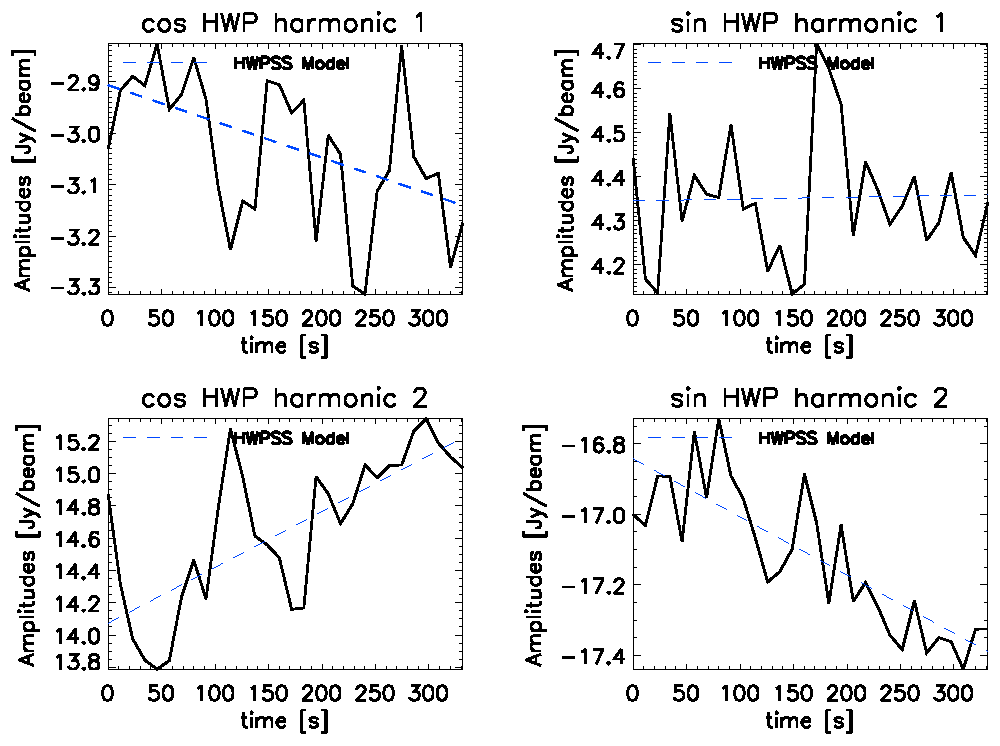
\includegraphics[%
%%   width=1.\linewidth,keepaspectratio]{figures/ampl_model.pdf}
%% \caption{ HWPSS template model (dotted blue lines), amplitudes fitted (black line) for a KID and 30 chunk of a scan of 3C 286.}
%%   \label{ampl_model}
%%   \end{center}
%%   \end{figure} 
 
%%In order to analyse the polarized data output we have developed a dedicated
%%polarization data reduction pipeline. $I$, $Q$, $U$ Stokes parameters maps in
%%sky coordinates are constructed by applying the following steps
%%
%%\subsubsection{Construct the template of the HWP modulation and removal of parasitic signal.} 
%%
%%
%%%Given a linear polarizing grid aligned with the +$Q$ state and a constant input polarization state, 
%%As discussed above the polarized power transmitted varies as a sinusoid with
%%angular frequency 4$\omega$, with amplitude $\propto$ $\sqrt{Q^2 + U^2}$ and
%%phase $\phi$ $\propto$ $arctan(U/Q)$.
%%
%%To have the polarized signal we extract this 4$\omega$ sinusoid component from
%%the signal recorded by a detector and reconstruct the incident $Q$ and $U$
%%states for making maps.
%%
%%Unfortunately the rotation of the HWP does not simply modulate optical
%%polarization signals into the detector timestream as sidelobes of
%%4$\omega$. Defects in the HWP or non-uniformities in its motion can be expected
%%to generate signals in the detector timestreams at arbitrary harmonics of its
%%rotation frequency.
%%
%%They are stationary in time, and thus appear as spikes in a signal period, which
%%can be completely described in terms of harmonic number, phase, and
%%amplitude. The periodic signal that is the combination of these harmonic terms
%%is called the HWP template.
%% 
%%%We fit this signal before proceeding with further analysis. 
%%Thanks to the synchronization of the detector KID with the acquisition software we can reconstruct the HWP rotation angle and we model the HWP-synchronous signal (HWPSS) \citep{johnson2007} as:
%%
%%\begin{eqnarray}
%% <h_{i}> &=& \sum\limits_{i=1}^N A_i cos(i\omega_{i}) + B_i sin(i\omega) \nonumber \\
%% 	     &+& A_{i}^{'} t cos(i\omega_{i}) + B_{i}^{'} t sin(i\omega_{i})
%% \label{hwpss}
%% \end{eqnarray}
%% A, B, A$^{'}$, B$^{'}$ represent the amplitudes of N = 9 harmonics considered. We call this estimator $<h_i>$ the HWP template. 
 
%% To probe the stationarity of the harmonics with time we plot in
%% Fig. \ref{time_drift} the ratio between the linear fit coefficients estimated on
%% the amplitudes variations with time and the HWP template amplitudes fitted $A$,
%% $B$ reconstructed by the Eq. \ref{hwpss}. This figure show the percentage HWP
%% template harmonics variation of $\sim$ 10$^{-3}$. The weak drift in time permits
%% to assume constant the content of this parasitic signal; the data are cleaned by
%% the subtraction of the template reconstructed.

We also observe a harmonics total power content correlated to the opacity
variation at 1mm channel, which is more affected by the atmospherical background
variation. This correlation is shown in
Fig. \ref{ampl_opac_1mm}. Fig. \ref{ampl_opac_2mm} shows the harmonics total
power content for the 2mm channel observations.
 
 \begin{figure}
  \begin{center}
  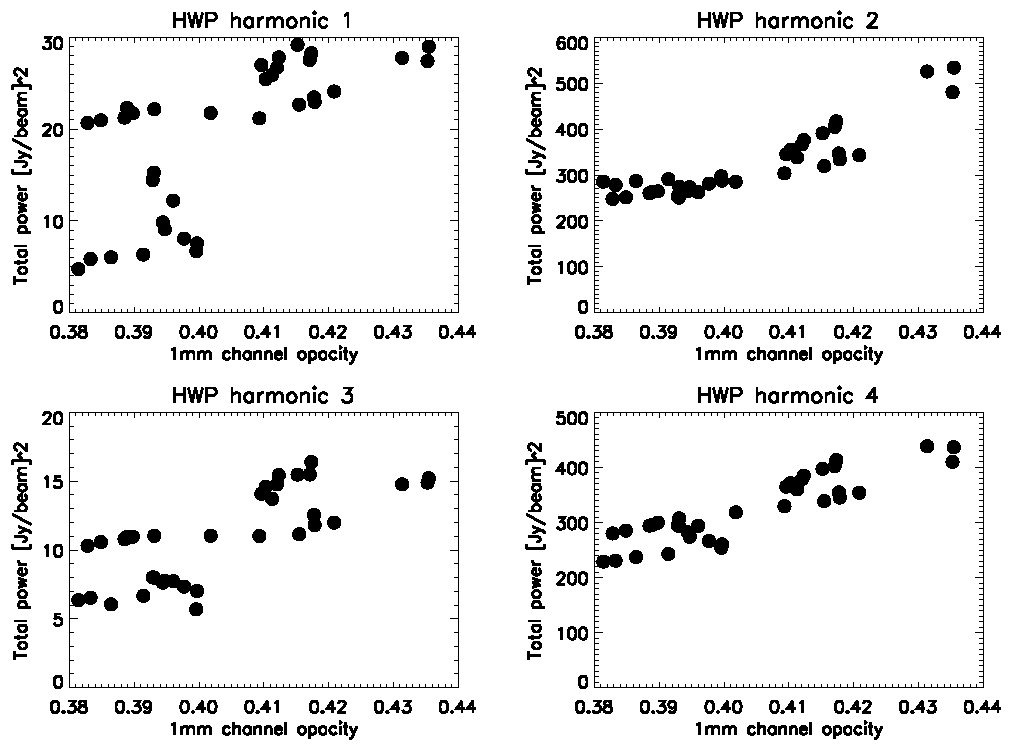
\includegraphics[%
  width=1.\linewidth,keepaspectratio]{figures/amplitudes_vs_opacity_1mm.pdf}
\caption{ Total power content for four harmonics of the HWP. The plots represent a KID of the 1mm matrix and the monitoring of the HWP template amplitudes for the quasar 3C 286 during three days of observation.}
  \label{ampl_opac_1mm}
  \end{center}
  \end{figure}
    
  \begin{figure}
  \begin{center}
  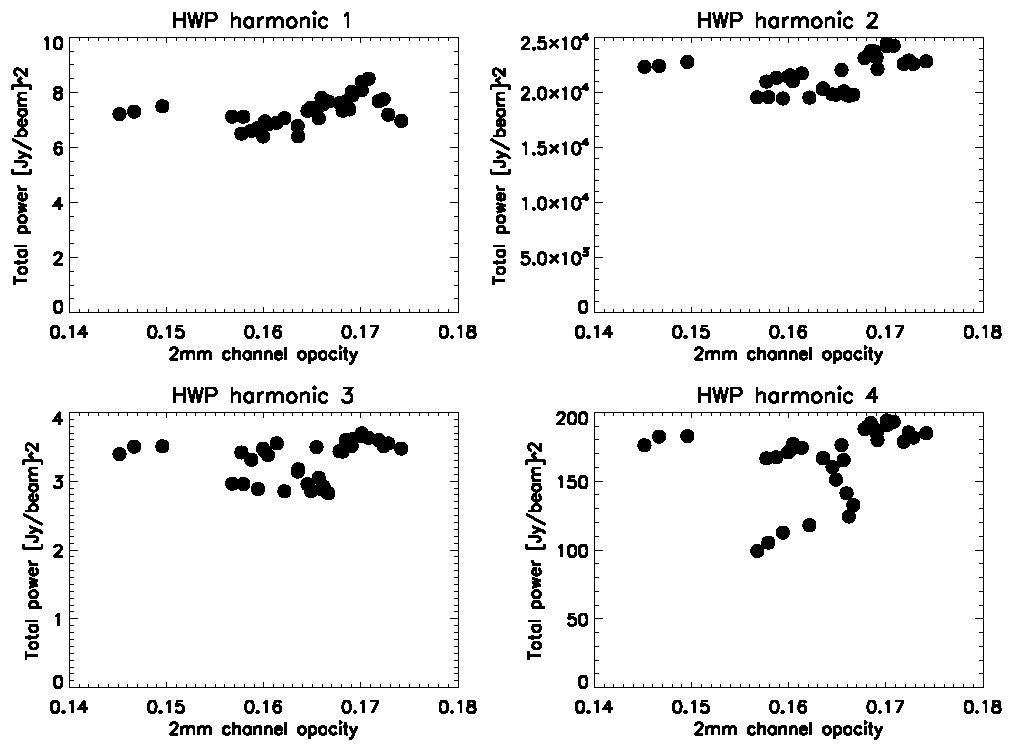
\includegraphics[%
  width=1.\linewidth,keepaspectratio]{figures/amplitudes_vs_opacity_2mm.pdf}
\caption{ Total power content for four harmonics of the HWP. The plots represent a KID of the 2mm matrix and the monitoring of the HWP template amplitudes for the quasar 3C 286 during three days of observation.}
  \label{ampl_opac_2mm}
  \end{center}
  \end{figure}

 
%% It is built to include terms linear in time to allow for the template amplitude
%% to drift in time which fit quite well the observed drift; the variations in the
%% HWP rotation frequency are naturally considered because the sinusoidal terms are
%% functions of the HWP orientation angle, not of time.
%% 
%% The procedure used in the data reduction software returns the HWP template
%% fitted in order to subtract it from the measured signal $m_k$, see
%% Eq. \ref{signal_polar}.
%% 
%% Fig. \ref{toi_i} (left) shows a timeline for a KID of Orion OMC-1 observation
%% scan, the raw data (black) are atmospheric turbulence affected with a modulated
%% parasitic synchronous signal at all harmonics of the mechanical rotational
%% frequency $\omega$, the blue line represents the raw data subtracted for the
%% synchronous signal template HWPSS.
%% 
%% A chunk of the timeline in Fig. \ref{toi_i} (left) is shown in Fig. \ref{toi_i}
%% (right) where the modulation is clear at several harmonics of the HWP rotational
%% frequency $\omega$. The linear spectrum on the middle show very well the
%% amplitudes of the harmonics 1$\omega$, 2$\omega$, 3$\omega$ and 4$\omega$ where
%% it is also located the polarized signal.

%\subsubsection{Construction of $Q$ and $U$ TOIs.}

%% \subsubsection{Time-ordered polarization informations (TOIPs) extrapolation.} 
%% To build the timelines TOIP (time-ordered polarization information) we use the
%% modulation/demodulation technique \citep{siringo2003}.  The modulation is given
%% by the rotating HWP and the $Q$ and $U$ timelines are extracted from the TOI by
%% demodulation using a phase-locked at the frequency of 4$\omega$ $\sim$ 12 Hz.

%% \subsubsection{Atmospheric noise and projection of the I, Q, U TOIs into I, Q, U maps}
%% Atmospheric emission dominates at low frequencies with a $1/f$ like spectrum but
%% the modulation of the polarized signal imposed by the HWP combined with the
%% scanning strategy allows us to shift the astrophysical signal away from the
%% largest atmospheric contribution \citep{johnson2007}.
%% 
%% Fig. \ref{spectre_iqu} evidences the importance of the rotational detection
%% mode. Spectra of the three timelines TOI $I$ (left), TOI $Q$ (middle) and TOI
%% $U$ (right) are shown.

The TOI $I$ spectrum shows a $1/f^\beta$ noise with $\beta$ $\sim$ -1.2 due to
the atmospherical fluctuations, the amplitude is time dependant. This noise
component affects all detectors and it is easily subtracted using the common
mode decorrelation.  On the middle and right of the Fig. \ref{spectre_iqu} are
shown the power spectra for TOIP $Q$ and $U$. The spectra are flats showing a
typical white noise spectrum $ < 1 Jy/\sqrt{Hz}$. The Q, U timelines could be
directly projected on maps. This shows the accuracy of this detection strategy.

%%For map making, the demodulation procedure also includes a band-pass filter with
%%high and low-pass edges at 0.01 and 2.9 Hz, respectively, that is used to reject
%%any out-of-band signals. In order to make a $n_{pix}$ map, all samples must be
%%taken into account to include noise correlations (in time and from pixel to
%%pixel) \citep{benoit2004}. Equation \ref{signal_polar} is generalized to:
%%
%%\begin{equation}
%%\mathbf{M} = \mathcal{A} \mathbf{S} + \mathbf{N} 
%% \end{equation}

%% where $\mathbf{M}$ is the time ordered vector of $n_{\rm t}$ x $n_{\rm kid}$
%% measures, $\mathbf{S}$ the (3 $n_{\rm pix}$) - vector Stokes map of the sky,
%% $\mathcal{A}$ the pointing matrix and $\mathbf{N}$ the $n_{\rm t}$ x $n_{\rm
%%   kid}$ noise vector. The least square best fit function is:
%% 
%% \begin{equation}
%% \mathbf{S} = (\mathcal{A}^{T} \mathcal{N}^{-1} \mathcal{A})^{-1} \mathcal{A}^{T} \mathcal{N}^{-1} \mathbf{M}
%%  \end{equation}
%% 
%% with covariance matrix
%% 
%% \begin{equation}
%% \Sigma = (\mathcal{A}^{T} \mathcal{N}^{-1} \mathcal{A})^{-1}
%%  \end{equation}
%% 
%%  The projection on maps follows the methods detailed in \citep{catalano2014,adam2014}.

%Nevertheless the time ordered data contain a significant instrumental signal which is synchronous with the rotation of the HWP, as shown in fig. \ref{toi_i}. The HWP synchronous signal is estimated and subtracted from the raw data, producing the time-ordered information (TOI). 


%When the noise is not correlated from one measurement to another,  $\mathcal{N}$ is diagonal and the inversion of large matrices can be solved. We therefore consider each pixel individually, computing the (3,3)- matrix  $\mathcal{A}^{T} \mathcal{N}^{-1} \mathcal{A}$ and the (3)-vector $\mathcal{A}^{T} \mathcal{N}^{-1} \mathbf{M}$.
  
%%\subsection{Intensity to polarization leakage}
%%In order to estimate the level of the instrumental polarization at the telescope
%%we have observed the planet, Uranus, which is expected to be unpolarized.  From
%%the $I, Q, U$ maps of Uranus, see Fig. \ref{uranus} we identify a systematic
%%effect fixed in NASMYTH coordinates which the cabin reference frame.


%% To first order we assume this effect as a leakage of total power into
%% polarization. In terms of instrumental polarization degree the systematic effect
%% at the peak of the leakage beam maps corresponds to 2 $\%$ and 3 $\%$ of the
%% intensity $I$ at 150 and 260 GHz, respectively.
%% 
%% As we have discussed above the power spectrum of the TOIP is consisting with a
%% flat spectrum. The negative and positive beam observed in the leakage maps
%% compensate each other and smooth the effect.  Taking a convolution between the
%% atmospherical spread signal, the Stokes intensity $I$ map with the
%% characteristic 1/f component of noise, and the leakage beam in $Q$ and $U$ we
%% found that the two component compensation drowning the effect in a white noise.
%%  
%% We have developed an algorithm to take into account for the effect on maps and
%% any additional instrumental polarization signal.  Let's call S$_k$ the
%% instantaneous measure of a kid and denote by a superscript $^N$ the Nasmyth
%% coordinates, we have:
%% 
%% \begin{eqnarray}
%% S_k &=& B_I * (I^N_0 + Q^N_0\cos2\alpha_{\rm Sky} + U^N_0\sin2\alpha_{\rm Sky}) \nonumber \\
%%        &+& L_{IQ}*I^N_0\cos2\alpha_{\rm Sky} + L_{IU} * I^N_0\sin2\alpha_{\rm Sky} + {\rm noise}
%% \label{eq_leak}
%% \end{eqnarray}
%% where $\alpha_{\rm Sky}$ accounts for the HWP angle and sky coordinates rotation and $B$ denotes
%% the instrumental beam. $L_{IX}$ the effective beam of the leakage. As Uranus can be considered a point source with respect to the {\it NIKA} FWHM, the $Q^N$ and $U^N$ maps give directly the $L^{\rm IQ}$ and $L^{\rm IU}$ beams. 
%% The algorithm used for the polarization leakage effect is:
%% \begin{enumerate}
%% \item Build a map of $I$, $Q$ and $U$ of the observed source in R.A. and
%%   Dec. This map can be the combination of multiple scans to have the best signal
%%   to noise S/N.
%% \item Rotate this map in Nasmyth coordinates to obtain $I_N$, $Q_N$ and $U_N$.
%% \item Deconvolve $I_N$ from the instrumental beam to have an estimate of
%%   $\hat{I}_0$ of the unprojected intensity.
%% \item Convolve $\hat{I}_0$ with the Uranus $Q^N$ and $U^N$ maps to obtain an estimation of the polarization leakage signal. 
%% \item Deproject these maps to produce timelines and subtract these timelines from the
%%   original data.
%% \item Project these corrected data onto final Stokes parameters maps.
%% \end{enumerate}
%% 
%% The deconvolution/convolution steps 3 and 4 are performed at the same time in Fourier
%% space:
%% 
%% \begin{equation}
%% (I^N_0*L_{IQ})(k) = I^N_0(k) \times L_{IQ}(k) \simeq I^N(k)/B_I(k)\times L_{IQ}(k)
%% \end{equation}
%% The ratio $L_{IQ}(k)/B_I(k)$ is tapered so that the division by decreasing terms
%% of $B_I(k)$ when $k$ increases is counterbalanced by the deaming of
%% $L_{IQ}(k)$. Once this correction is applied on Uranus polarization maps the instrumental residual polarisation is estimated to be below 0.1 $\%$ as shown in Fig. \ref{Uranus_corrected}. $I, Q, U$ maps are shown in order to compare directly with the maps uncorrected represented in Fig. \ref{uranus}.
%% 
%% In order to show the effect of the algorithm leakage correction we show the maps obtained at 150 GHz of the quasar 3C 273  shown in Fig. \ref{3c273_ex}, projected in RA, Dec coordinates. The maps show the systematic effect in the polarized maps $Q$ and $U$ (top) and the efficiency of our algorithm correction in the corrected maps on bottom.  
%% 

\section{Point source observations for calibration \label{calibration}}
During the polarization campaign on February the calibration procedure used was
the same discussed in section \ref{sec:pipeline}, the \emph{skydip} has been
performed with the operating rotating HWP and the polarization pipeline has been
used in order to have the TOI intensity Stokes vector $I$.

The calibration factor includes the correction for the reduced flux received by
the LEKIDs due to the warm wire-grid. The calibration uncertainty for point
sources on the final data is estimated to be 15 \% for the 1.25 mm channel and
10 \% for 2.05 mm channel, a list of main error sources is detailed in
\citep{catalano2014}. The FWHM of the beam are 13.5 and 18.4 arcsec at 260 GHz
and 150 GHz.

In order to cross check at the opacity correction and photometric calibration we
compare the results of four quasars (3C 273, 1749+096, 0851+202, 0415+379)
observed by {\it NIKA} and XPOl experiment \citep{thum2008} during a parallel
session of observation during the observational campaign on February 2015. In
the tab. \ref{tab:calib} we can see the consistency of {\it NIKA} results with
XPOl observations. The calibration error, reported in \citep{catalano2014} is of
the order of $\sim$ 10 $\%$ and is taken into account in the statistical
error. The K-correction is $\sim$ 1-2 $\%$ for the synchrotron spectra of
quasars, so it is negligible respect to the calibration error estimation.

%\begin{table*}
%\begin{center}
%\begin{tabular}{ccccccccc}
%\hline
%\hline
%Source & I flux Xpol 1.25 mm & I flux Xpol 3 mm &  I flux {\it NIKA}  1.25 mm& I flux {\it NIKA}  2.05 mm\\
% & [K] & [K] & [K] & [K]\\
%\hline
%3C273 & 0.614 $\pm$0.002      &  2.304 $\pm$ 0.002  & 0.60$\pm$ 0.09    &  1.35$\pm$0.23\\
%1749+096 & 0.201$\pm$0.001 & 0.558$\pm$0.001     & 0.15$\pm$0.03     &  0.26$\pm$0.06\\
%0851+202 & 0.384$\pm$0.002 & 0.989$\pm$0.001     & 0.31$\pm$0.06     &  0.57$\pm$0.13 \\
%0415+379 & 0.117$\pm$0.002 &  0.343 $\pm$0.001   & 0.122$\pm$0.025 &  0.238$\pm$0.055\\
%\hline
%\end{tabular}
%\end{center}
%\caption{Intensity flux results from the parallel session of observations between XPOl and {\it NIKA}.}
%\label{tab:calib}
%\end{table*}


\landscape
\begin{table}
\begin{center}
\caption{ Intensity and polarization fluxes, polarisation degree and angle for the quasars observed at 260 GHz and at 150 GHz during the campaign on February 2015. The {\it NIKA} angle uncertainty takes into account for both statistical and systematic error.}

\begin{tabular}{ccccccccccccc}
\hline
\hline
Source & I flux & Q flux &  U flux  & p & $\alpha_{Sky}$ & I flux & Q flux &  U flux  & p & $\alpha_{Sky}$ \\
            & [Jy] & [Jy] & [Jy] & [\%] & [$^\circ$] & [Jy] & [Jy] & [Jy] & [\%] & [$^\circ$] \\
            & 260 GHz & 260 GHz & 260 GHz & 260 GHz & 260 GHz & 150 GHz & 150 GHz & 150 GHz & 150 GHz & 150 GHz\\
\hline
3C279 &  8.51$\pm$0.97 &  0.260$\pm$0.005 & 0.79$\pm$0.09 & 9.8 $\pm$ 2.2 & 35.9$\pm$1.4(stat) $\pm$1.8(syst) &  12.4$\pm$1.4 &  0.51$\pm$0.06 &  1.05$\pm$0.12 &  9.5$\pm$2.2 & 31.9$\pm$1.8(stat)$\pm$1.8(syst) \\
3C273 &  6.3 $\pm$0.7 & -0.22 $\pm$ 0.01 & -0.009 $\pm$0.001 &  3.8$\pm$0.4 & -88.6$\pm$0.2(stat)$\pm$1.8(syst) & 10.04 $\pm$1.12 & -0.17$\pm$ 0.02 & -0.10$\pm$ 0.01 &  2.0 $\pm$ 0.5 & -74.1 $\pm$ 2.1(stat) $\pm$ 1.8(syst) \\
3C286 &  0.27$\pm$0.03 & 0.020$\pm$0.002 & 0.033$\pm$0.004 & 14.1$\pm$3.2 & 29.0$\pm$2.1(stat) $\pm$ 1.8(syst) & 0.51$\pm$0.10 & 0.037$\pm$0.004 & 0.05$\pm$0.01 & 12.9$\pm$2.9 &  27.7$\pm$2.1(stat) $\pm$ 1.8(syst) \\
3C345 &  1.08$\pm$0.12 & 0.035$\pm$0.002 & 0.003$\pm$ 0.004 & 3.2$\pm$ 0.7 & 2.7$\pm$0.4(stat) $\pm$ 1.8 (syst )&  1.82 $\pm$ 0.20 & 0.031$\pm$0.003 & 0.010$\pm$0.001 & 1.8$\pm$0.4 &  9.2$\pm$1.4(stat) $\pm$ 1.8(syst) \\
1749+096 & 1.64$\pm$0.19 & 0.005$\pm$0.004 & 0.063$\pm$0.007 &  3.9$\pm$0.9 & 43.0$\pm$0.3(stat) $\pm$ 1.8(syst) & 1.93$\pm$0.20 & -0.0016$\pm$0.0002 & 0.07$\pm$0.01 & 3.6$\pm$0.8 & 45.6$\pm$ 0.1(stat) $\pm$ 1.8(syst)  \\
0851+202 & 3.27$\pm$0.37 & -0.105$\pm$0.002 &  0.02$\pm$0.002 & 3.3$\pm$0.7 & 84.0$\pm$0.9(stat) $\pm$ 1.8(syst) &  4.36$\pm$0.51 & -0.10$\pm$0.01 & 0.08$\pm$0.01 & 2.9 $\pm$ 0.7 & 70.3 $\pm$2.3(stat) $\pm$ 1.8(syst)  \\
0923+392 & 2.04$\pm$0.23 & -0.002 $\pm$0.005 & -0.07 $\pm$ 0.01 & 3.3$\pm$0.7 & -45.8$\pm$0.1(stat) $\pm$ 1.8(syst) & 3.25$\pm$0.41 & -0.016$\pm$0.002 &  -0.09 $\pm$ 0.01 & 2.7$\pm$0.6 & -50.3$\pm$0.8(stat) $\pm$ 1.8(syst)  \\
0415+379 & 1.29$\pm$0.15 & 0.017$\pm$0.006 & -0.025$\pm$0.003 & 2.4$\pm$0.5 &  -28.4$\pm$2.1(stat) $\pm$ 1.8(syst) & 1.8$\pm$0.2 & 0.010$\pm$0.001 & -0.028$\pm$0.003 & 1.7$\pm$0.4 & -34.2$\pm$1.6(stat) $\pm$ 1.8(syst)\\
\hline
\end{tabular}
\label{tab:table_quasar}
\end{center}


\begin{center}
\caption{ Results of the parallel session of observation between XPOl and {\it NIKA} for polarization degree and angle for the quasars 3C273, 1749+096, 0851+202, 0415+379. The {\it NIKA} angle uncertainty takes into account for both statistical and systematic error.}
\begin{tabular}{cccccccccccc}
\hline
\hline
Source & p  & p  & p  & p  & $\alpha_{Sky}$ & $\alpha_{Sky}$ & $\alpha_{Sky}$  & $\alpha_{Sky}$\\
 & [$\%$] & [$\%$] & [$\%$] & [$\%$] & [$^\circ$] &[$^\circ$] &[$^\circ$]&[$^\circ$] \\
 & {\it NIKA} 1.25 mm & {\it NIKA} 2.05 mm & XPOl 1.3 mm & XPOl 3 mm & {\it NIKA} 1.25 mm  & {\it NIKA} 2.05 mm & XPOl 1.3 mm & XPOl 3 mm \\
 
\hline
3C273 & 3.8$\pm$0.4       & 2.0 $\pm$ 0.5 & 3.6$\pm$ 0.2  & 1.1$\pm$ 0.0 & -88.6$\pm$2.0 & -74.1 $\pm$ 3.9  & -76.8$\pm$ 1.6 & -37.8$\pm$ 0.9\\
1749+096 & 3.9$\pm$0.9 & 3.6$\pm$0.8 & 2.0$\pm$0.3      & 0.9$\pm$0.1 &  43.0$\pm$2.1 & 45.6$\pm$ 1.9 & -83.0$\pm$3.7 & 75.0$\pm$1.6 \\
0851+202 & 3.3$\pm$0.7 & 2.9 $\pm$ 0.7 & 2.8$\pm$0.3    & 1.1$\pm$0.0 & 84.0$\pm$2.7 & 70.3 $\pm$4.1 & -67.5$\pm$2.4  & -38.5$\pm$1.7 \\
0415+379 & 2.4$\pm$0.5 & 1.7$\pm$0.4 & 2.2$\pm$1.5     & 0.4$\pm$0.1 & -28.4$\pm$3.9  & -34.2$\pm$3.4 & 74.2 $\pm$19.3  & -14.2 $\pm$7.2\\
\hline
\end{tabular}
\label{tab:calib_degree}
\end{center}

\begin{center}
\caption{  Comparison of {\it NIKA}  results with other experiments.}
\begin{tabular}{ccccccccc}
\hline
\hline
Source & Experiment & Wavelength & p & $\alpha_{Sky}$ & Observation date & Comments\\
 & & & $[ \%]$&[$^\circ$]\\
\hline
3C279 &  SHARP Polarimeter &  350 $\mu$m, (3.5, 7, 13) mm &  10 $\%$-12 $\%$ & 32-41 &  2014, March & Variable source\\
           &  {\it NIKA}  & 1.25 mm & 9.8 $\pm$2.2 & 35.9 $\pm$3.2 & 2015, February  \\ 
	   &  {\it NIKA}  & 2.05 mm & 9.5 $\pm$2.2 & 31.9$\pm$3.9 & 2015, February\\ 
3C286 & XPOL & 1.3 mm & 14.4 $\pm$ 1.8 & 33.1 $\pm$5.7 & 2006-2012 & Calibration source\\
	   & CARMA & 1.3 mm & & 39.1$\pm$ 1 & 2015, May \\
	   & {\it NIKA}  &  1.25 mm &  14.1 $\pm$ 3.2 & 29.0 $\pm$ 3.9 & 2015, February\\	
	   & {\it NIKA}  &    2.05 mm &  12.9 $\pm$ 2.9 & 27.9 $\pm$3.9 & 2015, February \\
           & XPOL & 3 mm & 13.5 $\pm$0.3 & 37.3 $\pm$0.8 & 2006-2012 \\
3C273 & XPOL &   1.3 mm  &  3.6 $\pm$0.2 & -76.8$\pm$1.6 & 2015, February & Observational parallel session\\
        	   & {\it NIKA}   &   1.25 mm & 3.8$\pm$0.4 & -88.6$\pm$2.0 & 2015, February\\
           & {\it NIKA}  &    2.05 mm & 2.0$\pm$0.5 & -74.1$\pm$3.9 & 2015, February\\
           & XPOL &    3 mm    &   1.1$\pm$0.0 & -37.8$\pm$0.9 & 2015, February\\

\hline
\end{tabular}
\label{tab:tab_quasar}
\end{center}
\end{table}
\endlandscape

The Tab. \ref{tab:calib} show the consistency of {\it NIKA} flux measurements with XPOl results at 1mm.

To compare with other experiments we choose two of the quasars collection that we had, 3C 273 and 3C 286. In Fig. \ref{sed_3C286} we show the spectral energy density (SED) for the quasar 3C286, which is considered a primary calibrator for polarization experiments too. 

We plot the results obtained by PLANCK \citep{planckcatalogue}, ALMA \citep{almacalib}, XPOl \citep{xpol} and {\it NIKA} polarization campaign (February 2015).  We observe a synchrotron spectrum with a power law $\propto$ $\nu^{\rm \beta}$ with spectral index  $\beta$ $\simeq$ -1.007 $\pm$ 0.033. The fig. \ref{sed_3C273} presents the PLANCK and NIKA results for the quasar 3C273, the spectrum shows two power laws with spectral index $\beta_1$ $\simeq$ -0.29$\pm$0.05 and $\beta_2$ $\simeq$ -0.85$\pm$0.06. 

These two figures \ref{sed_3C273}, \ref{sed_3C286} shows the good photometric calibration effectuated and consistency of the {\it NIKA} results.


\begin{figure*}[h]
  \begin{center}
  \includegraphics[%
      width=0.33\linewidth,keepaspectratio]{figures/3C286_radec_corrected_I_1mm.pdf}
    \includegraphics[%
      width=0.33\linewidth,keepaspectratio]{figures/3C286_radec_corrected_Q_1mm.pdf}
        \includegraphics[%
      width=0.33\linewidth,keepaspectratio]{figures/3C286_radec_corrected_U_1mm.pdf}
       \includegraphics[%
      width=0.33\linewidth,keepaspectratio]{figures/3C286_radec_corrected_I_2mm.pdf}
   \includegraphics[%
      width=0.33\linewidth,keepaspectratio]{figures/3C286_radec_corrected_Q_2mm.pdf}
    \includegraphics[%
      width=0.33\linewidth,keepaspectratio]{figures/3C286_radec_corrected_U_2mm.pdf}
      \caption{Leakage corrected Stokes $I$, $Q$, $U$ maps of the quasar 3C 286
        observed at 260 (top) and 150 (bottom) GHz. The polarisation angle and
        degree are reported in the table \ref{tab:table_quasar}. {\nico La
          carte de I(1mm) est bizarre, non ?!}}
    \label{3c286_maps}
  \end{center}
\end{figure*}



\begin{figure*}
 \begin{center}
  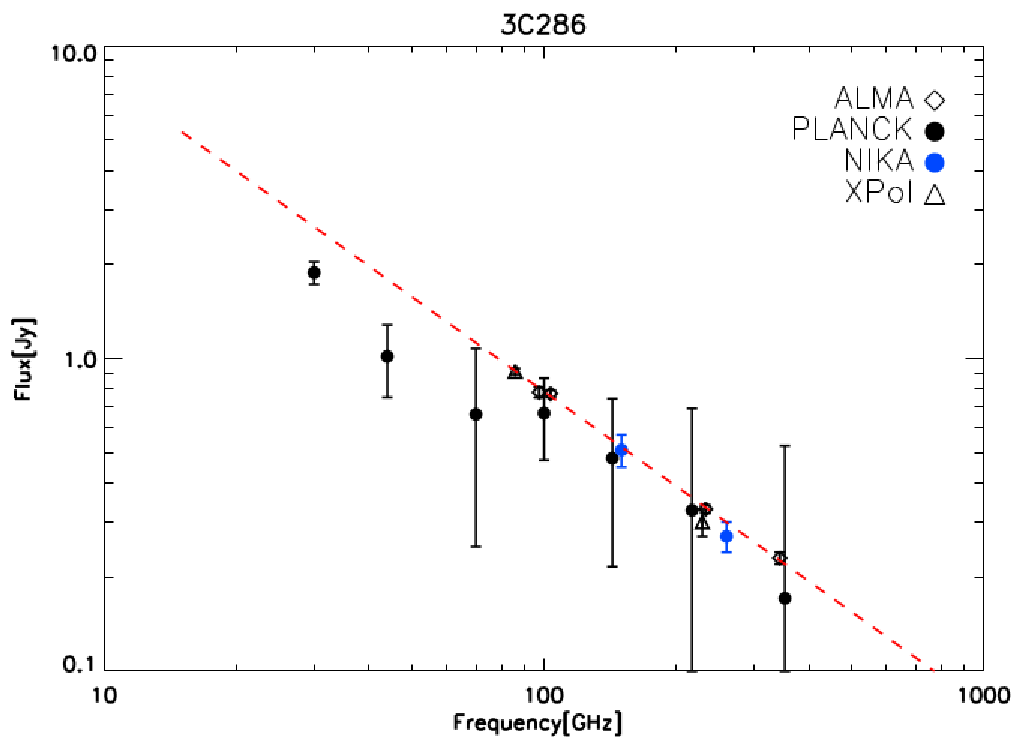
\includegraphics[%
  width=0.47\linewidth,keepaspectratio]{figures/ALMA_PLANCK_sed2_3C286.pdf}
  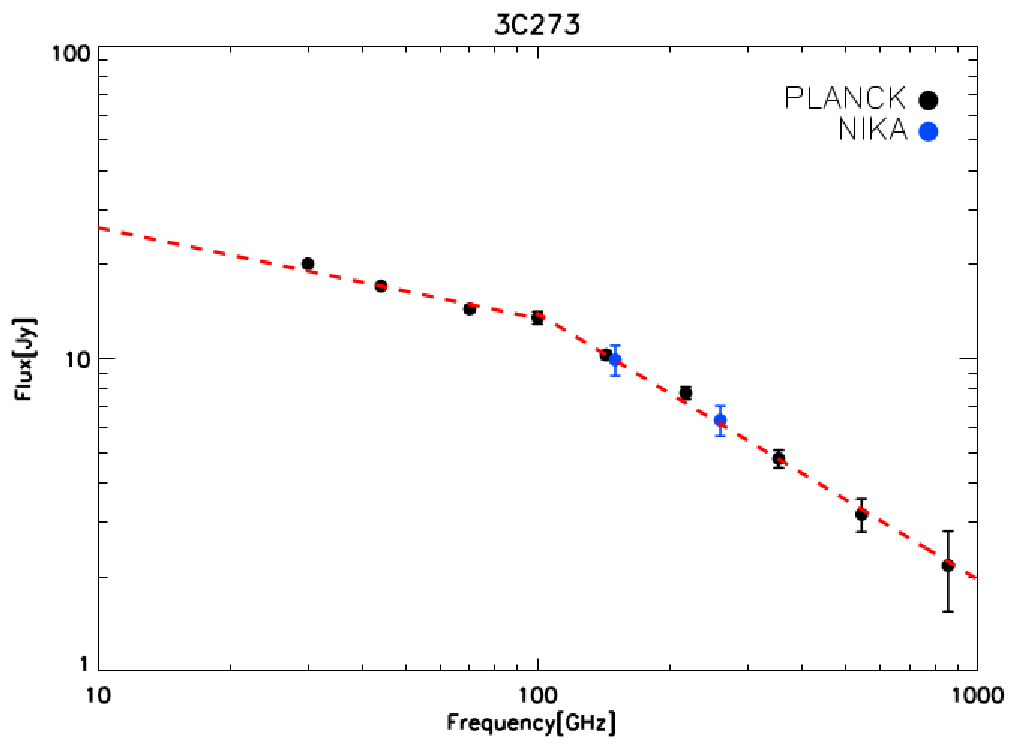
\includegraphics[%
  width=0.47\linewidth,keepaspectratio]{figures/ALMA_PLANCK_sed2_3C273.pdf}

  \caption{ Spectral energy density (SED) for the quasars 3C286 (left) and 3C273 (right). We consider data from Planck, ALMA, XPOL and \nika\ .}
  \label{sed_3C286}
 \end{center}
  \end{figure*}
  

%\begin{figure}
 %\begin{center}
  %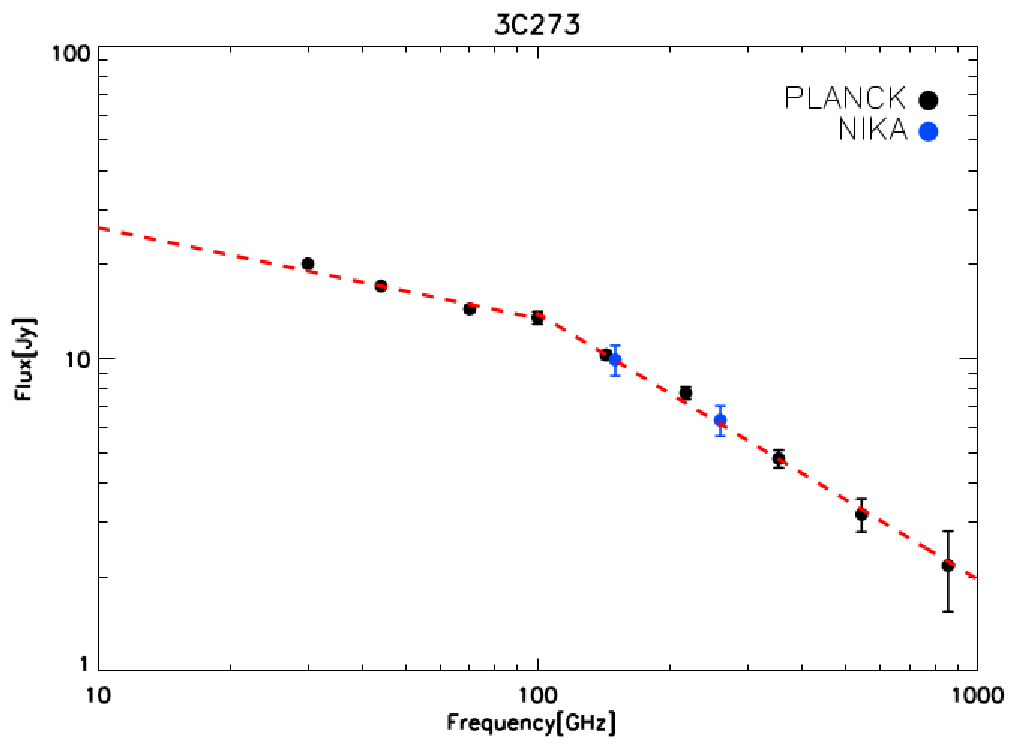
\includegraphics[%
 % width=0.66\linewidth,keepaspectratio]{figures/ALMA_PLANCK_sed2_3C273.pdf}
 % \caption{ 3C 273 spectral energy density (SED) of PLANCK and {\it NIKA} .}
 % \label{sed_3C273}
% \end{center}
 % \end{figure}
  
% Instrumental polarization and results ------------------------------------------------------------------------     

%\section{Polarimetry calibration}\label{polcalib}
To perform the calibration of the {\it NIKA} polarimeter we observed a selected list of quasars with low variability. Tab. \ref{tab:table_quasar} reporting the flux measured in $I, Q, U$, the polarization degree and angle on all maps of the quasars observed at both {\it NIKA} wavelengths. The results shown in this table are corrected for the leakage effect as discussed above.
The polarization degree $p$ is defined by 

\begin{equation}
p = \sqrt{(Q^2 + U^2)}/I
\end{equation}
with uncertainty:
\begin{equation}
\sigma p = p^{\rm -1} \sqrt{dQ^2Q^2 + dU^2U^2}
\end{equation}
and the polarization angle $\alpha_{\rm Sky}$
\begin{equation}
\alpha_{\rm Sky} = \frac{1}{2} \arctan\frac{U}{Q} ,  0 < \alpha_{\rm Sky} < \pi
\end{equation}
with statistical uncertainty:
\begin{equation}
\sigma\alpha_{\rm Sky}^{\rm stat} = \frac{1}{2}\{(Q^2+U^2)\sqrt{Q^2dU^2 + U^2dQ^2}\}^{\rm -1}
\end{equation}
The polarization angle is directly measured on the Sky considering the HWP zero defined with respect to the Nasmyth coordinates reference frame. A synchronized acquisition software provides the rotation angles of the HWP taken into account in the data analysis. As discussed above our precision in the determination of the HWP zero is 1.8$^\circ$, this is considered a systematic error in polarization angle measurements.
In the following sections we discuss the {\it NIKA} results comparing with previous observations. 

\subsection{3C 286}
3C 286 is a compact  steep-spectrum quasar at redshift z = 0.846. At centimeter wavelengths, 3C 286 represents the usual polarization calibrator; its position angle has been stable for decades \citep{perley&butler}. 

XPOl  polarimeter \citep{thum2008} has observed this quasar  at millimeter wavelengths for few years (2006-2012)  \citep{xpol}. The observations show a polarization angle (PA) of 3C 286 increasing slowly with frequency. 

The stability of this quasar in intensity and polarization in a large frequency range and the slow wavelength dependence identify it as a primary calibrator for polarization measurements. 

XPOl found a polarization angle $\alpha_{\rm Sky}$ = [37.3 $\pm$ 0.8]$^\circ$ and  $\alpha_{\rm Sky}$ = [33.1$\pm$5.7]$^\circ$, a polarization degree $p$= [13.5 $\pm$ 0.3] $\%$ and $p$ = [14.4$\pm$1.8] $\%$ at 86 and 229 GHz, respectively \citep{xpol}. Recent observation of 3C286 at 1.3 mm done by CARMA polarimeter \citep{carma} reports a polarization angle $\alpha_{\rm Sky}$ = [39.2$\pm$1]$^\circ$. 

{\it NIKA} polarimeter measures $\alpha_{Sky}$ = [29.0 $\pm$ 3.9]$^\circ$ and $\alpha_{Sky}$ = [27.7 $\pm$ 3.9]$^\circ$, a polarization degree $p$ = [14.1$\pm$3.2] $\%$ and $p$ = [12.9$\pm$2.9] $\%$ at 260 GHz and 150 GHz, respectively.

The agreement of the {\it NIKA} results with other millimeter experiments show the good performance of this new polarimeter in polarized light detection. 

\subsection{3C 279}
The blazar 3C 279 is one of the brightest and monitored flat-spectrum quasar and was the first object to exhibit apparent superluminal motion. The source of its strong radio to $\gamma$-ray emission  is  a  relativistic  jet  of  material  ejected  from  near  the black  hole  in  3C  279 \citep{apex3c279}.  

The {\it NIKA} results in intensity and polarization flux are reported in Tab. \ref{tab:tab_quasar}. For the polarization angles we found $\alpha_{Sky}$ = [35.9 $\pm$ 3.2]$^\circ$ and $\alpha_{Sky}$ = [31.9 $\pm$ 3.6]$^\circ$ and polarization degree $p$ = [9.8 $\pm$ 2.2] $\%$ and $p$ = [9.5 $\pm$ 2.2] $\%$ at 260 and 150 GHz, respectively. 
These results are in agreement with recent observations of the SHARP Polarimeter \citep{sharp3c279} done on March 2014 at 350 $\mu$m and 3.5, 7, 13 mm. Their observations report a polarization degree between 10-12 $\%$  and the polarization angles  between 32$^\circ$-41$^\circ$.


\subsection{Parallel session {\it NIKA} - XPOl}
On February 2015 we performed an observational parallel session with XPOl experiment. In this section we will discuss the results obtained by the data analysis from the two experiments. 
The results of this parallel session of the observations done between {\it NIKA} and XPOl are shown in Tab. \ref{tab:calib_degree}. 

There are some differences and incompatibilities between {\it NIKA} and XPOl data, most of them are likely due to expected trends between the different wavelengths of the instruments. At higher frequencies closer to the base of the jet the magnetic field tends to be more ordered. This can be explain why the polarization degree tends to increase towards higher frequency. 

The polarization angle is mainly affected by Faraday rotation which changes the angle as proportional $\lambda^2$. It is a weak effect at mm wavelengths, but clearly present in the more active AGNs. This affects more the 3 mm than 2 and 1 mm data. 

An other effect must also be expected due to changing optical depth with frequency which allows to see different parts of the jet where the magnetic field (and thus the polarization angle) may be different. 

\subsubsection{3C273 - 0851+202 - 1749+096 - 0415+379}
The quasar 3C 273 is the brightest and hence one of the best monitored AGN. Located at a distance of z = 0.158 \citep{3c273madsen}, at radio to millimeter and at $\gamma$-ray energies, flares from the relativistic jet dominate the variability of 3C 273 \citep{Abdo2010}. 

As Faraday rotation is proportional to $\lambda^2$  \citep{mckee} Faraday rotation measures (RMs) are expected to diminish at high frequencies. The core of the 3C273 shows this trend \citep{Attridge} at 86 GHz and explains the XPOl results. 

{\it NIKA} polarimeter measures {$\alpha_{Sky}$} = (-89.3 $\pm$ 3.2)$^\circ$ and $\alpha_{Sky}$ = (-74.1 $\pm$ 3.9)$^\circ$, $p$ = [3.8$\pm$0.4] $\%$ and $p$=[2.0 $\pm$ 0.5] $\%$ at 260 GHz and 150 GHz, respectively. 

XPOl measures {$\alpha_{Sky}$} = (-76.8 $\pm$ 1.6)$^\circ$  and {$\alpha_{Sky}$} = (-37.8 $\pm$ 0.9)$^\circ$, $p$ = [3.6$\pm$0.2] $\%$ and $p$ = [1.1$\pm$0.0] $\%$ at 229 GHz and 86 GHz, respectively.

This is the strongest source that we observed in parallel with XPOl and there is agreement between two experiments in both polarization degree and angle.

For the quasar 0851+202 there is a clear discrepancy in the angles between instruments for which we do not have an explanation. May be we have to check in the next observations. There is an agreement for both {\it NIKA} wavelengths.

For the quite variable quasar 1749+096 the {\it NIKA} 1 mm polarization degree is higher than XPOl that observes at 229 GHz.

The quasar 0415+379 is the weakest source at 1mm and however quite variable. It is too weak for XPOl measurement, we observe however an agreement between the two mm channel of {\it NIKA}.


% Extended sources section --------------------------------	
%OMC-1
\begin{figure*}
  \begin{center}
    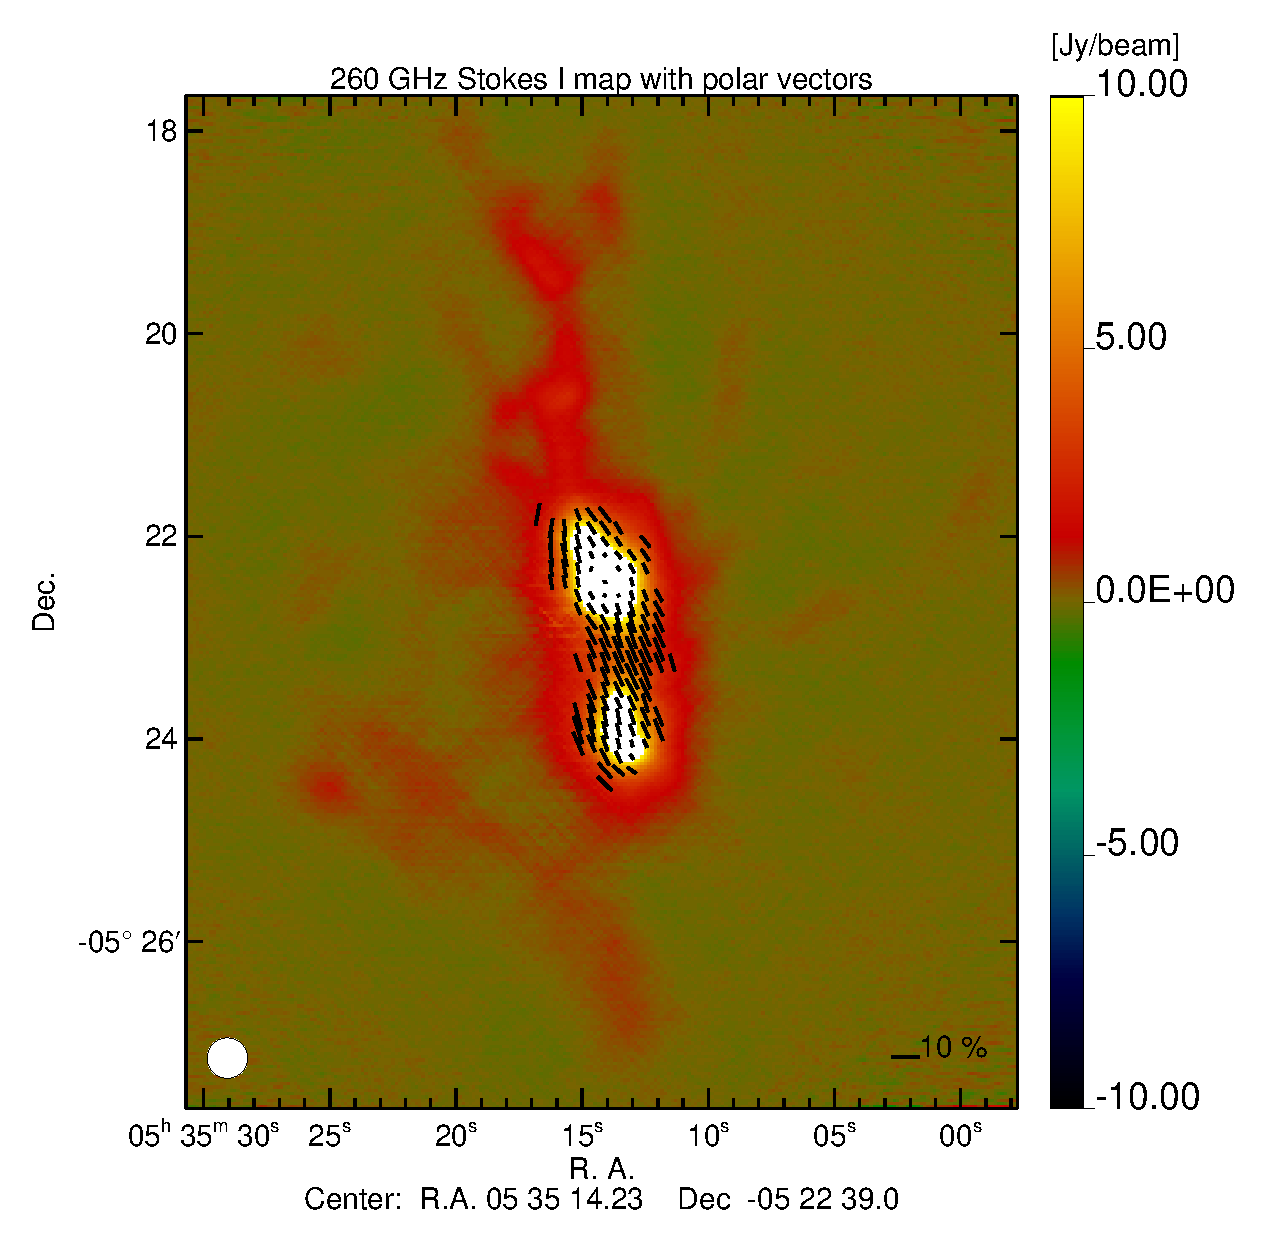
\includegraphics[%
  width=0.33\linewidth,keepaspectratio]{figures/Orion_I_map.pdf}
    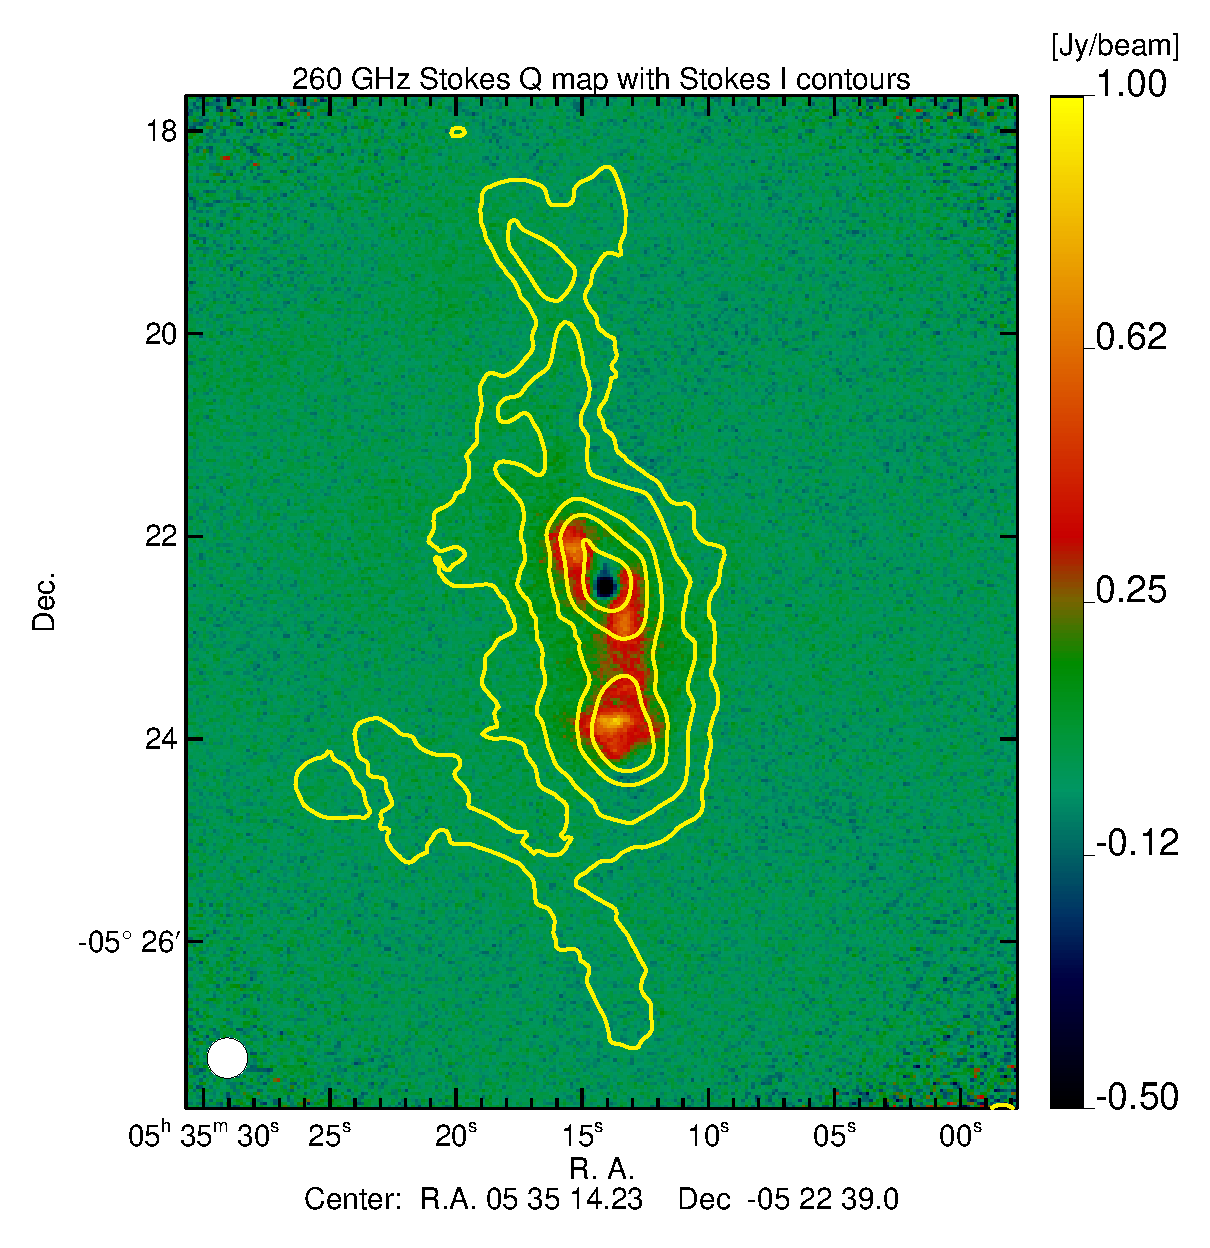
\includegraphics[%
  width=0.33\linewidth,keepaspectratio]{figures/Orion_Q_map.pdf}
   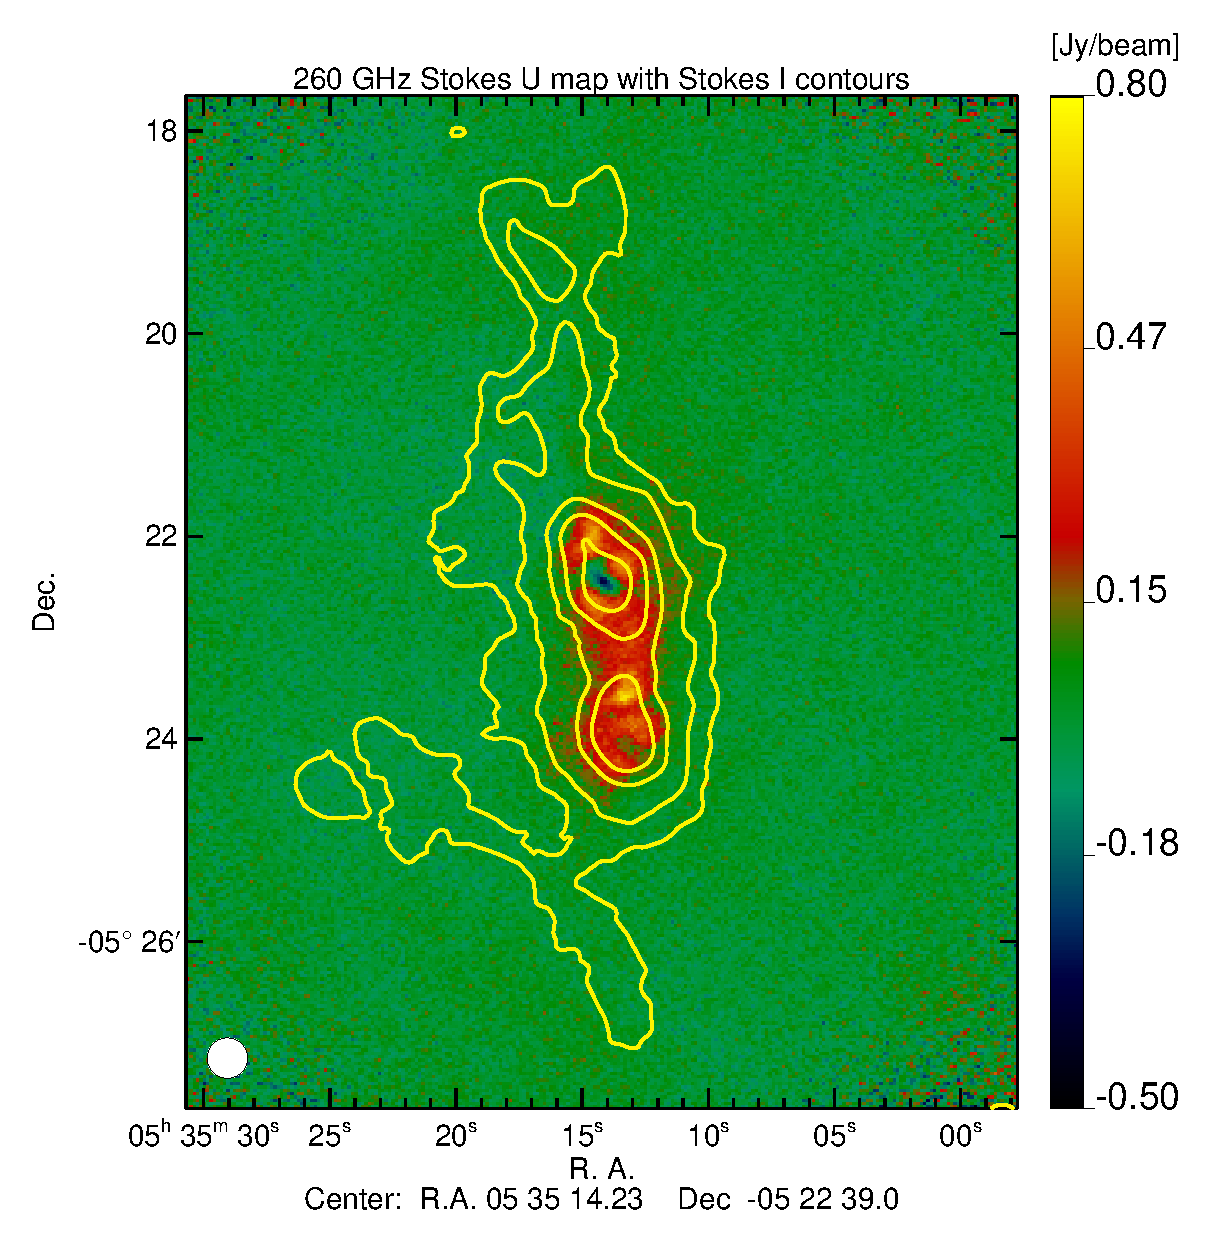
\includegraphics[%
  width=0.33\linewidth,keepaspectratio]{figures/Orion_U_map.pdf}
     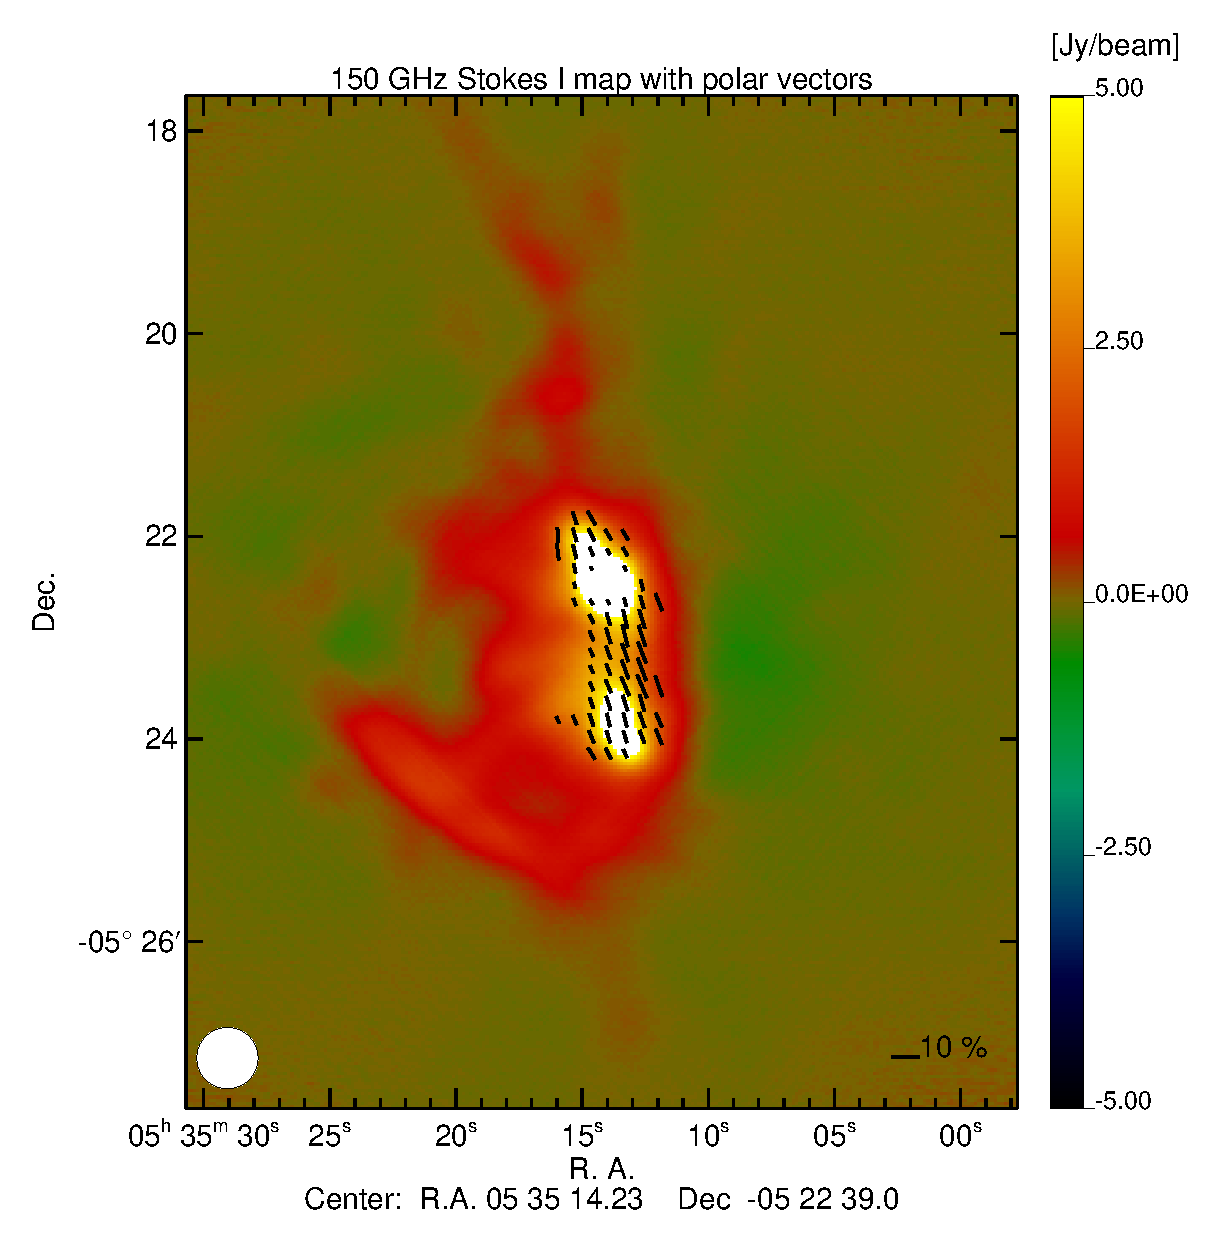
\includegraphics[%
  width=0.33\linewidth,keepaspectratio]{figures/Orion_I_map_2mm.pdf}
    \includegraphics[%
  width=0.33\linewidth,keepaspectratio]{figures/Orion_Q_map_2mm.pdf}
   \includegraphics[%
  width=0.33\linewidth,keepaspectratio]{figures/Orion_U_map_2mm.pdf}
\caption{ {\it NIKA} Stokes vector maps $I$, $Q$, $U$ (from left to right) of Orion OMC-1 observed at 260 GHz (top) and 150 GHz (bottom). The contours in the $Q, U$ maps have levels = (1, 2, 6, 10, 20, 38) Jy/beam at 260 GHz and (2, 4, 6, 8, 10, 14) Jy/beam at 150 GHz.}
  \label{Orion}
  \end{center}
  \end{figure*}

\begin{figure*}
  \begin{center}
  \includegraphics[%
  width=0.33\linewidth,keepaspectratio]{figures/M87_I_map.pdf}
   \includegraphics[%
  width=0.33\linewidth,keepaspectratio]{figures/M87_Q_map.pdf}
   \includegraphics[%
  width=0.33\linewidth,keepaspectratio]{figures/M87_U_map.pdf}
   \includegraphics[%
  width=0.33\linewidth,keepaspectratio]{figures/M87_I_map_2mm.pdf}
   \includegraphics[%
  width=0.33\linewidth,keepaspectratio]{figures/M87_Q_map_2mm.pdf}
   \includegraphics[%
  width=0.33\linewidth,keepaspectratio]{figures/M87_U_map_2mm.pdf}
   \caption{ M87 Stokes vectors $I$, $Q$, $U$, maps  at 260 GHz (top) and 150 GHz (bottom). The contours in $Q$, $U$ represent the $I$ map for each frequency. They start from 0.2 Jy/beam$^{-1}$ with steps of 0.2 Jy/beam$^{-1}$. }
    \label{M87_maps}
  \end{center}
  \end{figure*}



 \begin{figure*}
  \begin{center}
  \includegraphics[%
  width=0.33\linewidth,keepaspectratio]{figures/CYGNUSA_I_map.pdf}
   \includegraphics[%
  width=0.33\linewidth,keepaspectratio]{figures/CYGNUSA_Q_map.pdf}
   \includegraphics[%
  width=0.33\linewidth,keepaspectratio]{figures/CYGNUSA_U_map.pdf}
   \includegraphics[%
  width=0.33\linewidth,keepaspectratio]{figures/CYGNUSA_I_map_2mm.pdf}
   \includegraphics[%
  width=0.33\linewidth,keepaspectratio]{figures/CYGNUSA_Q_map_2mm.pdf}
   \includegraphics[%
  width=0.33\linewidth,keepaspectratio]{figures/CYGNUSA_U_map_2mm.pdf}
   \caption{ Cygnus A Stokes vectors $I$, $Q$, $U$, maps  at 260 GHz (top) and 150 GHz (bottom). The contours in $Q$, $U$ represent the $I$ map for each frequency. They start from 0.2 Jy/beam$^{-1}$ with steps of 0.2 Jy/beam$^{-1}$. }
    \label{cygnusa_maps}
  \end{center}
  \end{figure*}

	   
\section{Extended sources observations}\label{extended results}
The systematic effect correction discussed in section \ref{sec:pipeline} is also applied to the observations presented in this section on Orion OMC-1, M87 and Cygnus A. 

\subsection{Orion OMC-1}
The core of OMC-1, containing the Becklin-Neugebauer (BN) object and the Kleinmann-Low (KL) nebula, is an ideal region for polarimetric study of the thermal dust emission. In the background molecular cloud, the KL Nebula is the  peak from farinfrared to millimeter wavelengths on the OMC-1 ridge.
%The Orion Molecular Cloud (OMC) is the closest region of high-mass star-formation to the Sun, at $\sim$ 450 pc, and has consequently been much studied. 

The most prominent region in maps of the molecular gas is the OMC1 cloud, which contains several luminous star-forming cores \cite{chini1997} and a large number of young stars. 
In Fig. \ref{Orion_scuba} we show the maps of Orion OMC-1 obtained by SCUPOL instrument \citep{scubapol} at 850 $\mu$m. The contours represent the {\it NIKA} map obtained at 1.25 mm. We observe a bit shift between the two maps may be due to some pointing error in the specific observation session. 

If we compare the polarization intensity IPOL in Fig. \ref{Orion_scuba} on right with the polarization intensity  $IPOL$ = $\sqrt{Q^2 + U^2}$ obtained by {\t NIKA} observation in Fig. \ref{Orion_ipol} there is a consistency in the shape of the polarized regions. 
\begin{figure}
  \begin{center}
    \includegraphics[%
  width=1.\linewidth,keepaspectratio]{figures/NIKAvsScuba.pdf}
  \caption{ \NIKA\ Stokes $I$ at 260 GHz with SCUPOL map contours at 850 $\mu m$. The \NIKA\ map is shifted by $\sim$ 10 arcsec to match the SCUPOL map.}
  \label{Orion_scuba}
  \end{center}
  \end{figure}
  
In fig. \ref{Orion} we present the Orion OMC-1 maps of Stokes vectors $I$, $Q$, $U$ observed at both frequencies and corrected for the systematic effect previously discussed. The peak flux of the OMC1 emission in the Orion A molecular cloud is about 45.8 Jy/beam and 14 Jy/beam at 260 GHz and 150 GHz, respectively. 

The polarization angle and degree calculated with the average of the Stokes parameters are $\alpha_{Sky}$ = (21.3 $\pm$ 3.6)$^\circ$ and $p$ = (4.0 $\pm$ 0.8) $\%$  and  $\alpha_{Sky}$ = (22.1 $\pm$ 2.6)$^\circ$ and $p$ = (6.0 $\pm$ 0.9) $\%$ at 150 GHz and 260 GHz, respectively. 

Previous observations \citep{polka_apex} found the polarization angles in this star formation region $\sim$ 30$^\circ$.
The leakage maps found for this source represented in fig. \ref{Orion_leakage} show a reduced leakage effect compared to point source polarization degree. In fig. \ref{orion_vector} we show the Stokes vector $I$ with the vectors indicating the orientation of the polarization angle.

 
\subsection{M87}
M87 (also designated 3C274, NGC 4486, and Virgo A) is a giant
elliptical galaxy \citep{dev76} located near the 
core of Virgo cluster. 
Its nucleus is a radio and X-ray source, and from it emanates an
optical jet. It is estimated to be 16 Mpc from the earth \citep{mou80}. The core and jet can be seen at all wavelength 
from radio to X-rays.

Radio galaxies serve as a probe of their environments, providing means
to study the pressure, density, temperature, and magnetic strength, {\it
etc.} of the extragalactic medium (IGM) or intra-cluster
medium (ICM). 

The galaxy M87 is more studied at lower frequencies than the {\it NIKA} ones in order to study the physics of the filaments, the polarization 
degrees of the filaments are very high near the limit of synchrotron 
emission at this frequencies. At {\it NIKA} frequencies the galaxy appears with its core and the surrounding lobes. 

The M87 maps of Stokes vectors $I$, $Q$, $U$ observed at both frequencies by {\it NIKA} polarimeter instrument are shown in fig. \ref{M87_maps}. The peak flux of the $I$ map is $\sim$ 0.6 Jy/beam $\sim$ 1.5 Jy/beam at 260 GHz and 150 GHz, respectively. The leakage maps found for this source are shown in fig. \ref{M87_leakage}. 

The polarized intensity at 150 GHz shown in Fig. \ref{M87_ipol} suggests a synchrotron emission of the M87 lobes.  The polarized emission at 260 GHz is quite weak. 

 Fig. \ref{m87_vector} show the Stokes vector $I$ with the vectors indicating the orientation of the polarization angle at both frequencies.  They suggest the existence of  large scale ordered magnetic field {\bf B} in the radio lobes of M87.

\subsection{Cygnus A}
Cygnus A is a typical radio galaxy with twin jets of plasma emanating from its nucleus and forming two extended, radio- emitting lobes. 
It is  the most powerful Fanaroff- Riley II (FRII) radio galaxy in the local environment.
It has been well studied in terms of spatial resolution as it lies
at a distance of 227 Mpc. The global properties of the object are
reviewed in the literature.  

At low radio frequencies, the synchrotron emission
from the two giant lobes dominate \citep{1974MNRAS.166..305H}. At higher frequencies the
hotspots (working surfaces in the lobes) and the galaxy core become more prominent.
The southern and northern hotspots are respectively 50 and 70 arcsec from the core.
The complex structure of Cygnus A can be well explained by assuming that Cygnus A consists of two components which are polarized in opposite directions \citep{1967ApJ...150L..15S}, \citep{1966SvA....10..214S}, \citep{1968ApJ...151...53M}.

The {\it NIKA} Stokes parameters $I, Q, U$ maps of Cygnus A at 260 GHz (top) and 150 (bottom) GHz are presented in
the first and second row of Fig. \ref{cygnusa_maps}.  
The  unpolarized core of the source in the $Q$ and $U$ maps show the low level of instrumental polarization which affects polarization measurements and show the polarization of the jets with an opposite orientation of the polarization angle, as expected.

As expected, the
two hot spots and the galaxy core dominate the signal at the {\it NIKA}
frequencies. The peak flux of the $I$ map is $\sim$ 1.7 Jy/beam and $\sim$ 3 Jy/beam at 260 GHz and 150 GHz, respectively. 

The leakage maps found for this source are shown in Fig. \ref{cygnusa_leakage}, the effect is comparable to the quasar leakage effect, for Cygnus A appears as a compact source at {\it NIKA} frequencies. 

The polarization intensity at both frequencies is shown in Fig. \ref{cygnusa_ipol}. In Fig. \ref{cygnusa_vector} we show the Stokes vector $I$ with the vectors indicating the orientation of the polarization angle. 




%The hot spots present a spectral index (right map on the row) in
%the range -1.5 to -2.0, which is consistent with synchrotron emission but
%steeper than the value found by \citet{1998MNRAS.301..935R}, which is $\sim

%-1$. The galaxy core shows a flatter spectrum from -0.6 to -1.0, which is
%consistent with previous estimates from \citet{1999IAUS..194..179L}.
 
 \section{Conclusions}
This paper has shown the first polarization measurements with Kinetic Inductance Detectors technology. The efficiency of the polarization system adopted, consisting of an achromatic rotating Half Wave Plate plus a polarizer, has been demonstrated in detection of the polarization of few quasars, Orion OMC-1 molecular cloud and the radio galaxies M87 and Cygnus A. 
 
 A systematic leakage effect of total intensity into polarization shows up at the 3\% level for point sources and 2\% for extended sources. 
 We have been able to correct for it using calibration scan on Uranus on all observations shown in the section \ref{sec:polar_pipe}.
 
 {\it NIKA} was the test bench of {\it NIKA}2 camera, which observes at the same frequencies of {\it NIKA} with improved main performance and covering a Field of View (Fov) of 6.5 arcminutes. {\it NIKA} has been installed at the IRAM 30 meter telescope in Spain on October 2015 and it will be opened to public observations in late 2016. 
 
 {\it NIKA}2 has polarization capability at 260 GHz; the warm rotating HWP is placed in front of the {\it NIKA}2 cryostat and and the polarizer is mounted in the 100 mK stage of the cryostat splitting the two orientations of the linear polarization on two matrix of thousands of pixels.
 
The {\it NIKA}2 polarization channel will provide high angular resolutions observations of Galactic regions dust emission and would be clarify the understanding of the magnetic fields role in star formation process. 



\bibliography{biblio}
% \begin{figure*}
%  \begin{center}
%   \includegraphics[%
%    width=0.24\linewidth,keepaspectratio]{figures/Orion_IQ_1mm.pdf}
%    \includegraphics[%
%  width=0.24\linewidth,keepaspectratio]{figures/Orion_IU_1mm.pdf}
%  \includegraphics[%
%    width=0.24\linewidth,keepaspectratio]{figures/Orion_IQ_2mm.pdf}
%    \includegraphics[%
%  width=0.24\linewidth,keepaspectratio]{figures/Orion_IU_2mm.pdf}
%  \caption{ From left to right Orion OMC-1 intensity to polarisation leakage maps $IQ$, $IU$ at 260 GHz and at 150 GHz.}
%  \label{Orion_leakage}
%  \end{center}
%  \end{figure*}
  

%\begin{figure*}
%  \begin{center}
%        \includegraphics[%
%  width=0.4\linewidth,keepaspectratio]{figures/Orion_ipol_1mm.pdf}
%     \includegraphics[%
%  width=0.4\linewidth,keepaspectratio]{figures/Orion_ipol_2mm.pdf}
%     \caption{ Polarisation intensity maps at 260 GHz (left) and 150 GHz (right) of the molecular cloud Orion OMC-1. }
%    \label{Orion_ipol}
%  \end{center}
%  \end{figure*}



 % M87
  
    
  % \begin{figure*}
 % \begin{center}
  % \includegraphics[%
  %  width=0.24\linewidth,keepaspectratio]{figures/M87_IQ_1mm.pdf}
   % \includegraphics[%
  %width=0.24\linewidth,keepaspectratio]{figures/M87_IU_1mm.pdf}
  %\includegraphics[%
 %   width=0.24\linewidth,keepaspectratio]{figures/M87_IQ_2mm.pdf}
   % \includegraphics[%
 % width=0.24\linewidth,keepaspectratio]{figures/M87_IU_2mm.pdf}
  %\caption{ From left to right M87 intensity to polarization leakage maps $IQ$, $IU$ at 260 GHz and at 150 GHz.}
  %\label{M87_leakage}
 % \end{center}
 % \end{figure*}
  
  %\begin{figure*}
  %\begin{center}
  %\includegraphics[%
 % width=0.48\linewidth,keepaspectratio]{figures/M87_ipol_1mm.pdf}
 % \includegraphics[%
 % width=0.48\linewidth,keepaspectratio]{figures/M87_ipol_2mm.pdf}
  %  \caption{ M87 polarization intensity maps at 260 GHz (left) and 150 GHz (right). }
   %   \label{M87_ipol}
  %\end{center}
  %\end{figure*} 
 
  % Cygnusa
  

  
 %  \begin{figure*}
 % \begin{center}
 % \includegraphics[%
 %  width=0.24\linewidth,keepaspectratio]{figures/Cygnus_A_IQ_1mm.pdf}
 %   \includegraphics[%
 % width=0.24\linewidth,keepaspectratio]{figures/Cygnus_A_IU_1mm.pdf}
 %\includegraphics[%
 %   width=0.24\linewidth,keepaspectratio]{figures/Cygnus_A_IQ_2mm.pdf}
 %   \includegraphics[%
 % width=0.24\linewidth,keepaspectratio]{figures/Cygnus_A_IU_2mm.pdf}
 % \caption{ From left to right Cygnus A intensity to polarization leakage maps $IQ$, $IU$ at 260 GHz and at 150 GHz.}
 % \label{cygnusa_leakage}
%  \end{center}
%  \end{figure*}
  
%  \begin{figure*}
%  \begin{center}
%  \includegraphics[%
%  width=0.48\linewidth,keepaspectratio]{figures/Cygnus_ipol_1mm_NIKA.pdf}
%  \includegraphics[%
%  width=0.48\linewidth,keepaspectratio]{figures/Cygnus_ipol_2mm_NIKA.pdf}
%   \caption{ Cygnus A polarization intensity maps at 260 GHz (left) and 150 GHz (right). }
%      \label{cygnusa_ipol}
%  \end{center}
%  \end{figure*} 
 
  % Projection of vectors------------------
  
% \begin{figure*}
%  \begin{center}
%  \includegraphics[%
%  width=0.42\linewidth,keepaspectratio]{figures/map_I_1mm_vector_M87.pdf} 
%  \includegraphics[%
%  width=0.42\linewidth,keepaspectratio]{figures/map_I_2mm_vector_M87.pdf} 
%    \caption{ M87 Stokes vector $I$ intensity with polarization vectors at 260 GHz (left) and 150 GHz (right).}
%  \label{m87_vector}
%   \end{center}
%  \end{figure*}

%\begin{figure*}
%  \begin{center}
%  \includegraphics[%
%  width=0.42\linewidth,keepaspectratio]{figures/Cygnusa_map_I_1mm_vector.pdf} 
%  \includegraphics[%
%  width=0.42\linewidth,keepaspectratio]{figures/Cygnusa_map_I_2mm_vector.pdf} 
%    \caption{ Cygnus A Stokes vector $I$ intensity with polarization vectors at 260 GHz (left) and 150 GHz (right).}
%	\label{cygnusa_vector}
%   \end{center}
%  \end{figure*}

 
  
  %-----------------------------------------------------
  


%\pagebreak

        
\end{document}
